\documentclass[12pt,a4paper, usenames, dvipsnames]{article}
\usepackage{graphicx}
\usepackage{xcolor}


\usepackage[ngerman]{babel}
\usepackage[utf8]{inputenc}
\usepackage{mathtools}
\usepackage{amsmath}
\usepackage{amssymb}
\usepackage{geometry}
\usepackage{tikz}
\usepackage{float}
\usepackage{verbatim}

\usepackage{amsthm}
\newtheorem{definition}{Definition}

\usepackage[nottoc]{tocbibind}

\usepackage[onehalfspacing]{setspace}

\usepackage{stmaryrd}

\usepackage{microtype}

\usepackage{booktabs}

\usepackage{hyperref}
\hypersetup{
    colorlinks=true,
    linkcolor=black,
    filecolor=black,      
    urlcolor=blue,
    citecolor=black
}

\usepackage{subfigure}

\usepackage[compact]{titlesec}     


\usepackage[center]{caption}


\pagestyle{plain}

\usepackage[backend=biber]{biblatex}

\addbibresource{references.bib}

\newcommand{\Gtwo}{\ensuremath{G_{2\times 2\times 2}}}

\newcommand{\Gthree}{\ensuremath{G_{3\times 3\times 3}}}

\newcommand{\Ttwo}{2$\times$2$\times$2-}

\newcommand{\Tthree}{3$\times$3$\times$3-}

\clubpenalty = 10000
\widowpenalty = 10000
\displaywidowpenalty = 10000


\geometry{
  paper=a4paper, % Change to letterpaper for US letter
  top=3cm, % Top margin
  left=2cm, % Left margin
  right=3cm, % Right margin
  %showframe, % Uncomment to show how the type block is set on the page
}

\setlength{\parindent}{0em}

\setlength{\parskip}{1.3ex}

\pagenumbering {arabic} 

\titlespacing*{\section}{0pt}{10ex plus 1ex minus .2ex}{4.3ex plus .2ex}









\begin{document}




\begin{titlepage}
	\centering
	{\scshape\LARGE Technische Universität Dortmund \par}
	Fakultät für Informatik \par
	Lehrstuhl 14 für Software Engineering \par
	\vspace{1cm}
	{\scshape\Large Bachelorarbeit \par }
	\vspace{1.5cm}
	{\huge\bfseries  Gruppentheorie des \\ 2$\times$2$\times$2 Zauberwürfels und dessen Lösungsalgorithmen \par}
	\vspace{2cm}
	{\Large\itshape Pina Kolling\par}
	\vspace{0.5cm}
	{Abgabe: Mai 2021 \par }
	\vfill
	betreut von\par
	Dr. \L ukasz \textsc{Czajka} \par 
	und \par 
	M. Sc. Christoph \textsc{Stahl} 

	\vfill

% Bottom of the page
	{\large \today\par}
\end{titlepage}

\begin{singlespace}
\tableofcontents
\thispagestyle{empty} 
\end{singlespace}


\thispagestyle{empty} 



\newpage

\setcounter{page}{1} 
%

%
%
%
%
%=======================================================================================================
%
%
%
%
%
\section{Einleitung}

Der \Tthree Zauberwürfel ist ein mathematisches Drehpuzzle, das 1974 von dem ungarischen Professor Er\~{n}o Rubik erfunden wurde. Er wollte damit seinen Studenten helfen, dreidimensionale Probleme zu verstehen. 
Der sogenannte \textit{Rubik's Cube} wurde dann weltweit verkauft und 1982 fand in Budapest sogar die erste Weltmeisterschaft statt. \cite{RC}
Im Jahr 1981 hat \textit{Rubik} dann das Patent für den \Ttwo Würfel angemeldet \cite{patent}.

%
%
%
%
%=======================================================================================================
%
%
%
%
\subsection*{Motivation} \addcontentsline{toc}{subsection}{\protect\numberline{}Motivation}




Der \Tthree Würfel wurde mathematisch schon viel untersucht. 
Die \textit{God's Number} -- das ist die maximal mögliche Anzahl der nötigen Drehungen zur Lösung -- wurde oft berechnet und durch neue Algorithmen verbessert. 
Die Berechnung der \textit{God's Number} des \Tthree Cubes ist wesentlich anspruchsvoller und dadurch auch interessanter als die des \Ttwo Würfels. 

Der \Tthree Würfel wurde schon mehrfach als Gruppe dargestellt, während der \Ttwo Würfel
noch nicht umfangreich als Gruppe untersucht wurde. Ziel dieser Arbeit ist es, das Wissen des \Tthree \textit{Cubes} auf den \Ttwo \textit{Cube} zu übertragen.

Wer die Lösungsalgorithmen der \Ttwo Würfels selber herleiten möchte, sollte dies vor dem Lesen dieser Arbeit tun, da diese hier teilweise erklärt und genutzt werden.

%
%
%
%
%=======================================================================================================
%
%
%
%
\subsection*{Ausblick} \addcontentsline{toc}{subsection}{\protect\numberline{}Ausblick}

Im Folgenden wird zuerst der Aufbau des \Ttwo \textit{Cubes} beschrieben und danach werden die mathematischen Grundlagen der Gruppentheorie erklärt, auf denen diese Arbeit aufbaut. 
In Kapitel \ref{8} wird die Gruppe des \Ttwo Würfels definiert und bewiesen. 
Darauf folgt dann eine Beschreibung der Würfelkonfiguration und der Untergruppen des \textit{Cubes}. 
Am Ende werden die validen Konfigurationen des Würfels behandelt und danach findet sich ein Kapitel über die Lösungsalgorithmen.

%
%
%
%
%
%
%=======================================================================================================
%
%
%
%
%
%
\newpage
\section{Der \Ttwo Würfel}

In diesem Kapitel werden die Grundlagen des \Ttwo \textit{Cubes} erklärt. Zuerst wird der Aufbau und die Terminologie des Würfels erläutert. Dann wird kurz auf die Unterschiede zwischen dem \Ttwo und dem \Tthree Würfel eingegangen. 
Außerdem werden die Grundzüge des Würfels definiert und erklärt. Darauf basieren alle späteren Algorithmen. 


%
%
%
%
%
%
%=======================================================================================================
%
%
%
%
\subsection*{Terminologie} \addcontentsline{toc}{subsection}{\protect\numberline{}Terminologie}

Diese Arbeit befasst sich mit dem \Ttwo Zauberwürfel, deshalb sind Terminologie und Aufbau des \textit{Cubes} eine Grundlage für die weiteren Kapitel.
Im Folgenden wird die Terminologie und der Aufbau des Würfels erklärt.



\begin{description}


\item[\Ttwo Würfel] (auch Zauberwürfel oder \textit{Cube}) 

Der Würfel setzt sich auch acht kleinen Würfeln zusammen.
In Abbildung \ref{3} ist er links verdreht und rechts im gelösten Zustand zu sehen. Der gelöste Zustand wird auch als Startkonfiguration bezeichnet.
Bei der Startkonfiguration (auch Grundposition, Grundstellung) des \Ttwo Würfels hat jede Seite 4 Farbflächen einer Farbe. Der Würfel ist dann gelöst.  
Bei dem verdrehten Würfel sind die Steine des Würfels an anderen Positionen und anders ausgerichtet.
\begin{figure}[h]
\centering
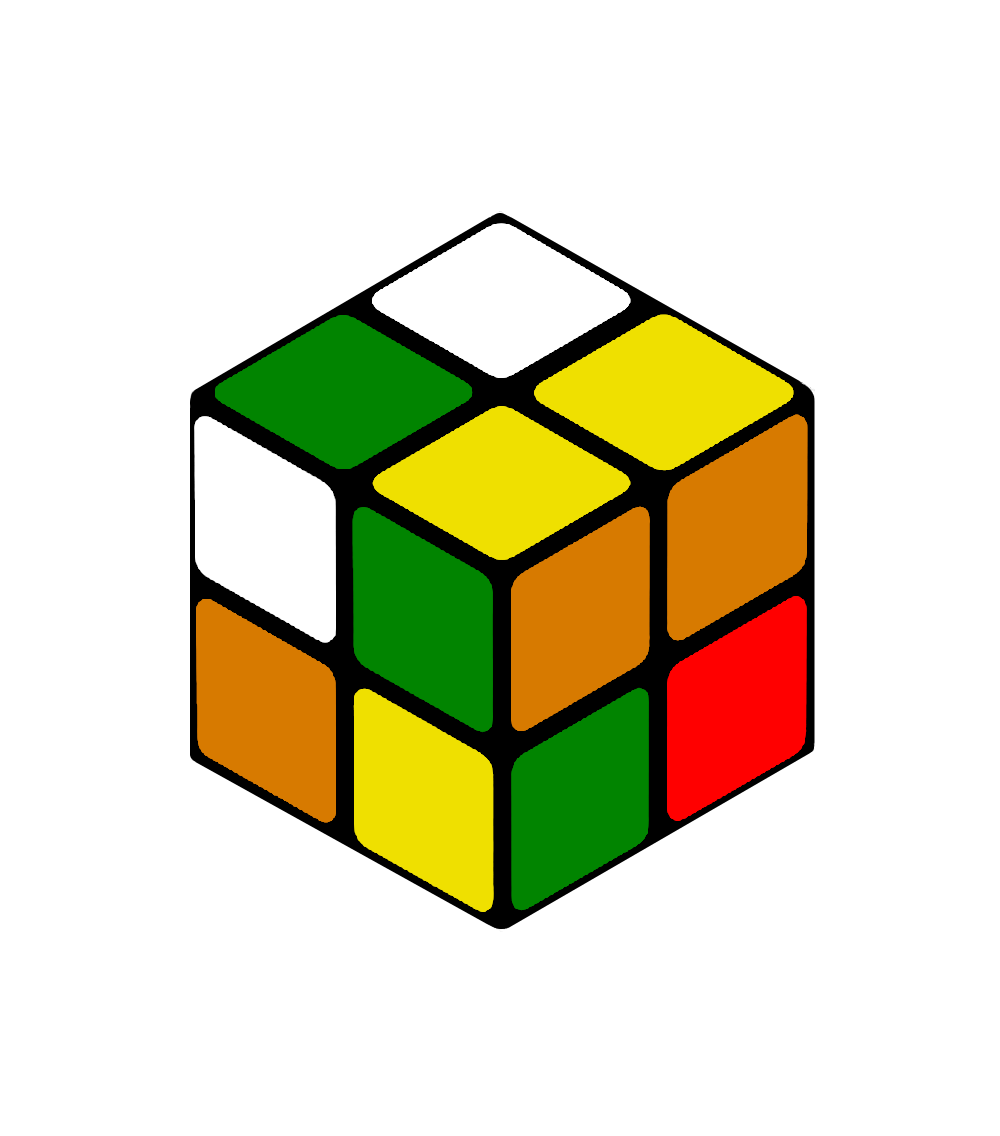
\includegraphics[scale=0.1]{2x2scrambled.png}
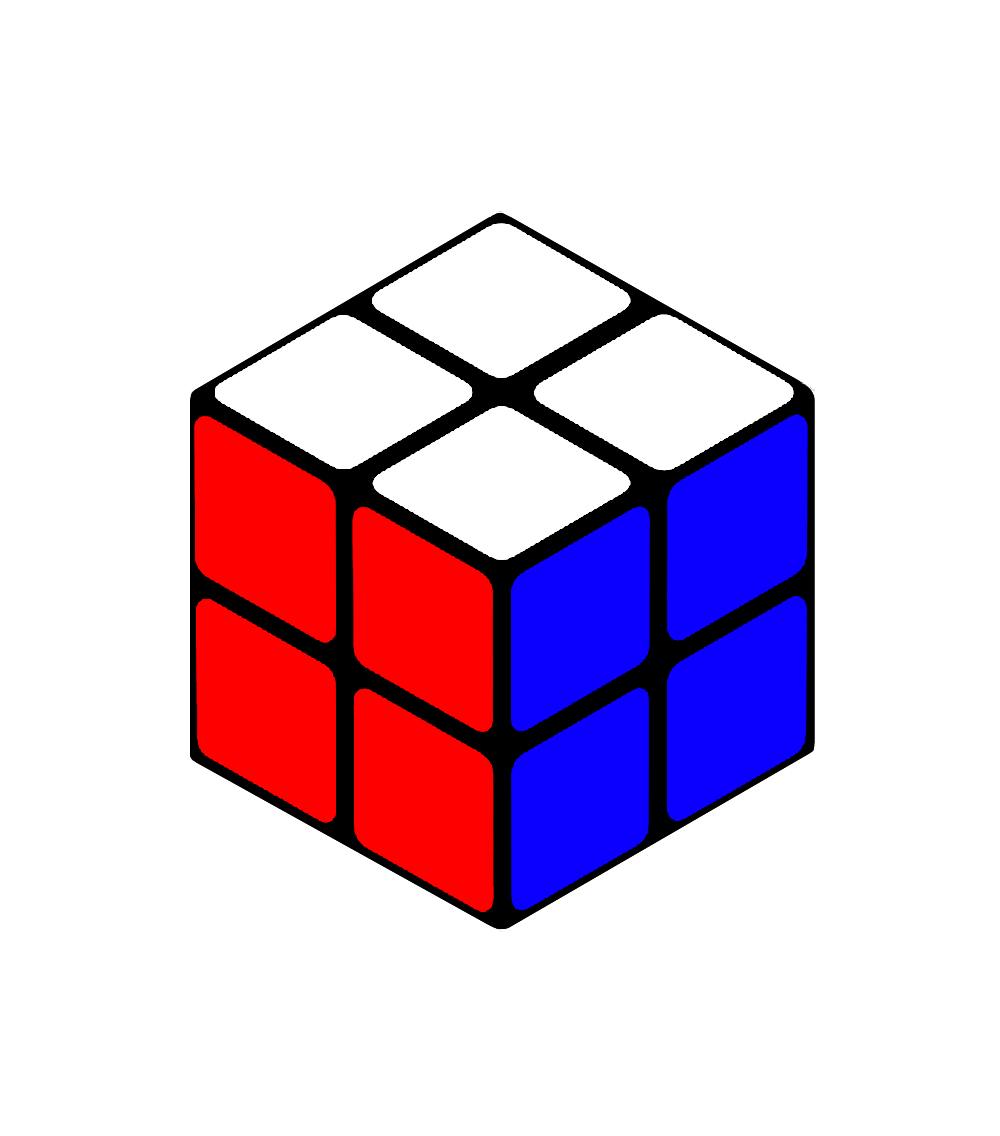
\includegraphics[scale=0.1]{2x2solved.png}
\caption[ungelöster und gelöster \Ttwo Würfel]{ungelöster und gelöster \Ttwo Würfel}
\label{3}
\end{figure}


\item[Eckstein und Farbfläche] \ \\
Ein \Ttwo Würfel besteht aus acht Ecksteinen (links in Abbildung \ref{4}), die jeweils drei Farbflächen (rechts in Abbildung \ref{4}) haben. Ein \Ttwo Zauberwürfel hat also 24 Farbflächen. Die verschiedenen Farbpaare, die sich jeweils gegenüberliegen, sind weiß und gelb, rot und orange, grün und blau.
\begin{figure}[h]
\centering
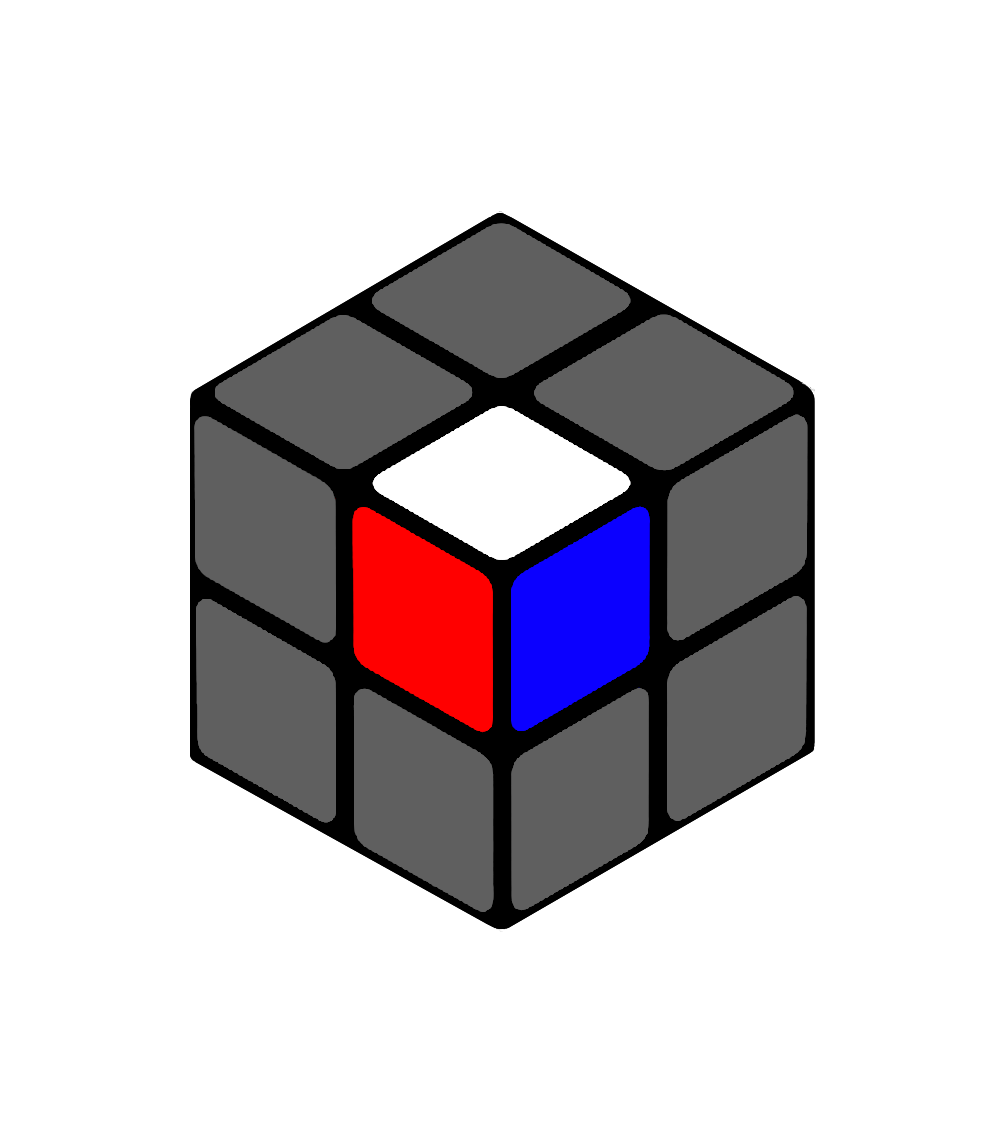
\includegraphics[scale=0.1]{2x2stein.png}
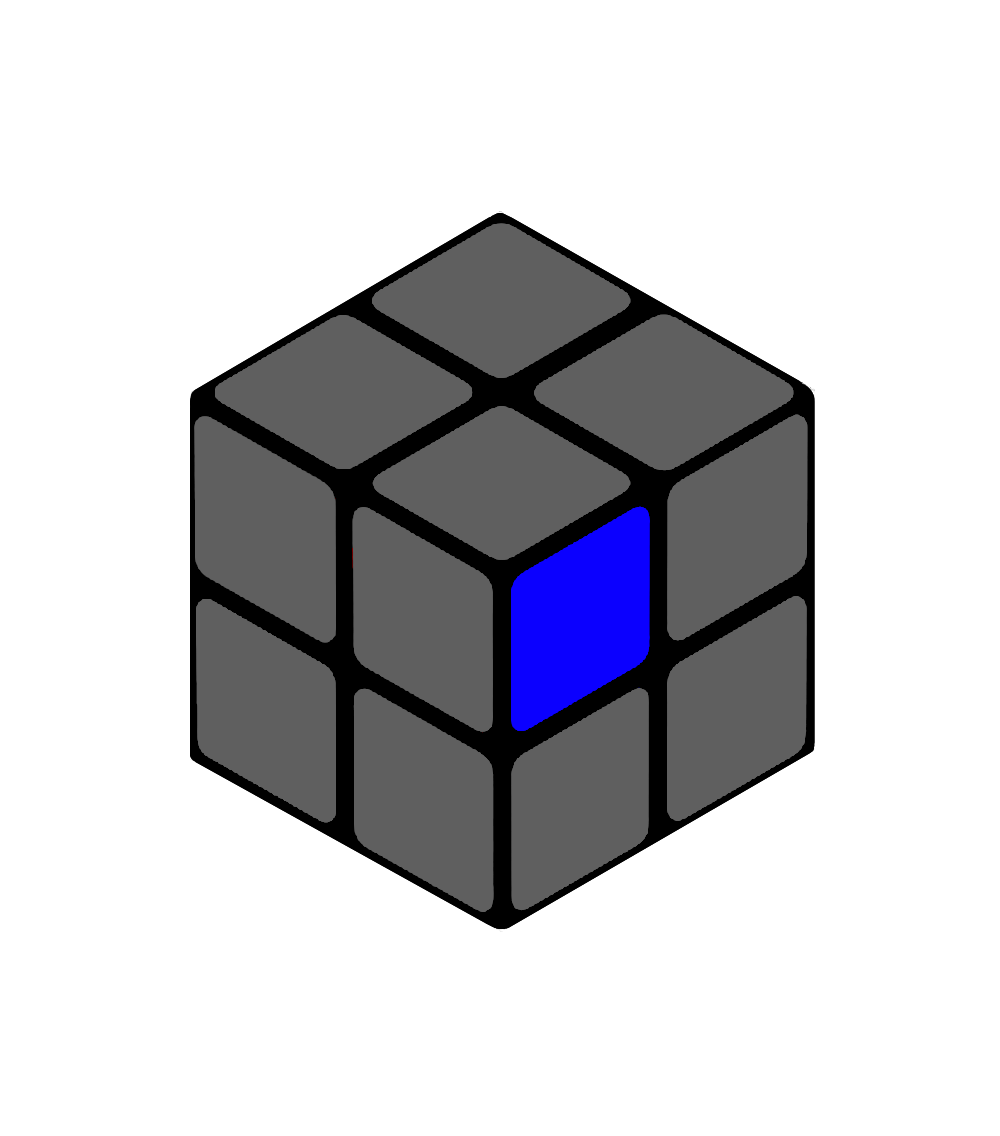
\includegraphics[scale=0.1]{2x2farbflaeche.png}
\caption[Eckstein und Farbfläche des Würfels]{Eckstein und Farbfläche des Würfels}
\label{4}
\end{figure} 


\newpage

\item[Seite] \ \\
Der \Ttwo und der \Tthree Würfel haben sechs Seiten (bestehend aus jeweils vier Farbflächen) und somit sechs Farben. Die weiße Seite wird üblicherweise als obere Seite bezeichnet. \\
\begin{figure}[h]
\centering
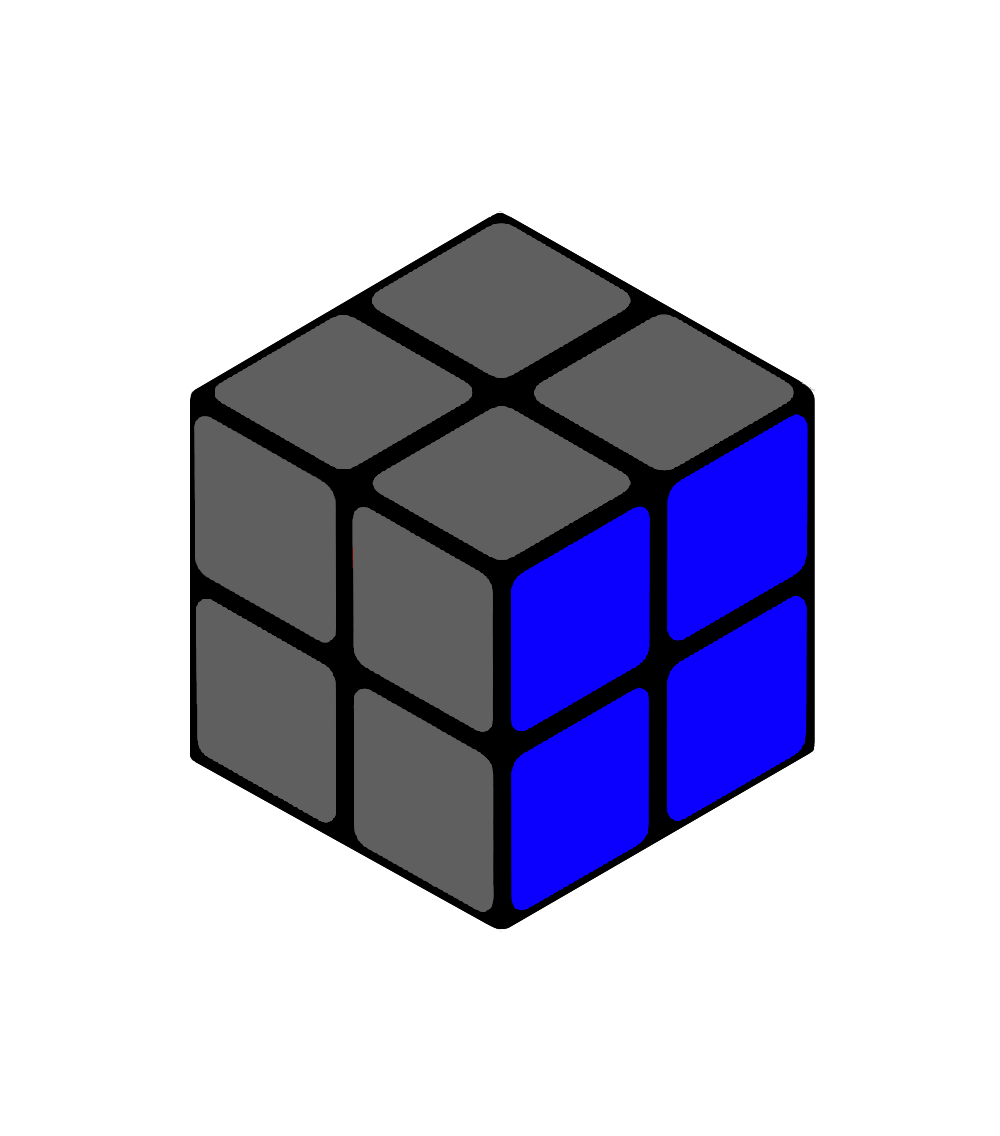
\includegraphics[scale=0.1]{2x2seite.png}
\caption[Seite des Würfels]{Seite des Würfels}
\end{figure}


\item[\Tthree Würfel] \ \\
Wesentlich bekannter als der \Ttwo \textit{Cube} ist der \Tthree \textit{Cube}. Er besteht aus 26 Steinen. In Abbildung \ref{5} sieht man ihn links ungelöst und rechts in der Startkonfiguration.

\begin{figure}[h]
\centering
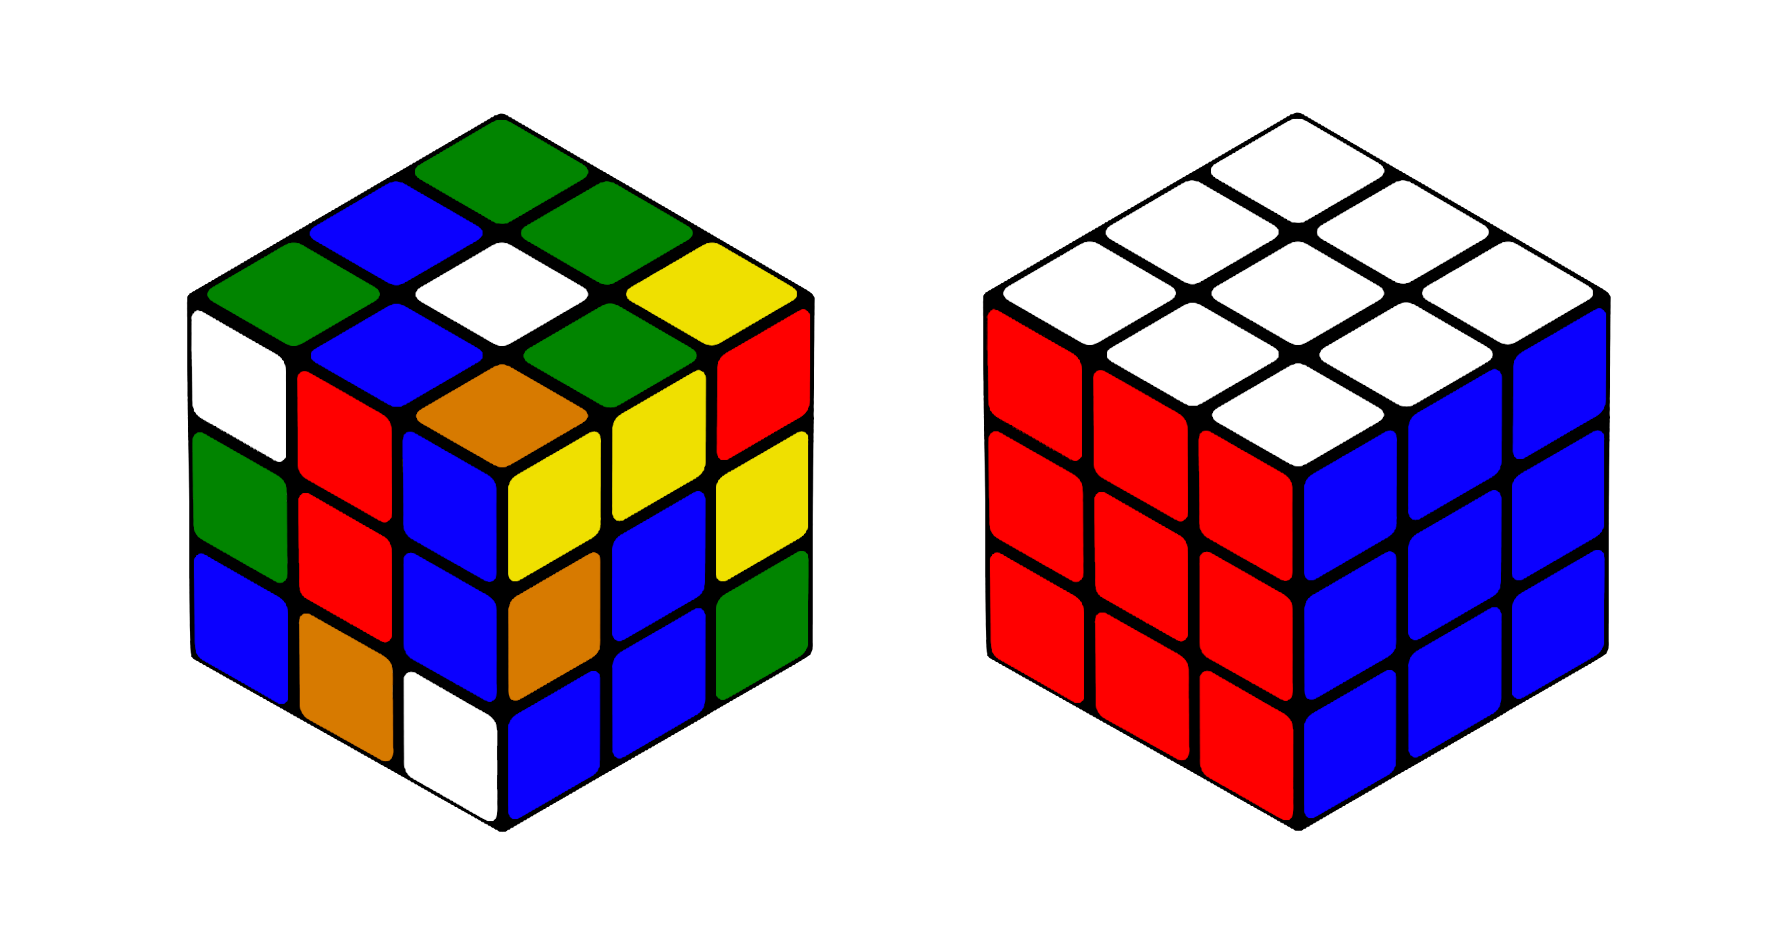
\includegraphics[scale=0.11]{3x3_sc_so.png}
\caption[ungelöster und gelöster \Tthree Würfel]{ungelöster und gelöster \Tthree Würfel}
\label{5}
\end{figure}

\newpage
\item[Eck- und Kantsteine] \ \\
Im Gegensatz zum \Ttwo hat der \Tthree Würfel Kantsteine und Mittelsteine (s. Abbildung \ref{6}).
\begin{figure}[h]
\centering
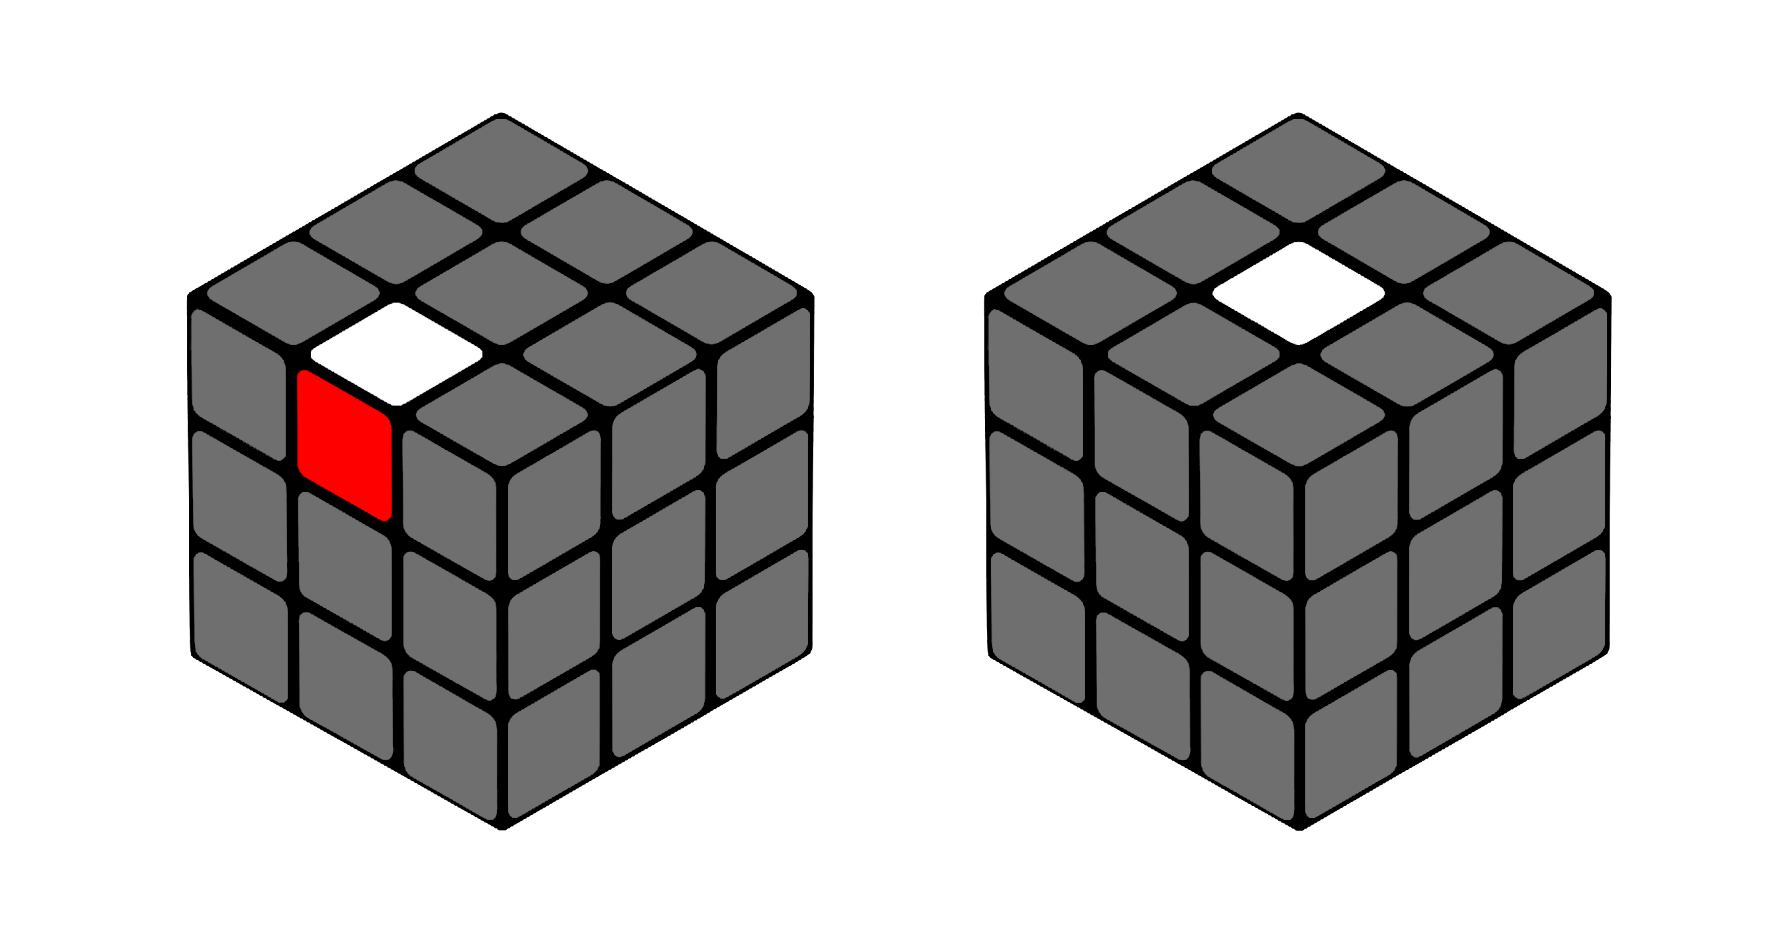
\includegraphics[scale=0.11]{mittelkant.png}
\caption[Kant- und Mittelsteine]{Kant- und Mittelsteine}
\label{6}
\end{figure}
Das besondere an den Mittelsteinen des \Tthree Würfels ist, dass sie bei einer Drehung der Ebenen (also bei Zügen des Würfels) nicht verändert werden. Somit ist beim \Tthree Würfel die obere Seite immer fest zu stellen: Die obere Seite hat immer das weiße Mittelstück in der Mitte. 


\end{description}

Beim \Ttwo \textit{Cube} gibt es keine eindeutige Oberseite. Es ist also möglich, dass die aktuelle Konfiguration einer vermeintlich anderen Konfiguration entspricht, bei der nur eine andere Seite nach oben gehalten wird.
Die Ausrichtung des gesamten Würfels ist bei dem \Tthree Würfel also eindeutig vorgegeben, während sie beim \Ttwo Würfel gedreht werden kann.  
Das muss beachtet werden, da in dieser Arbeit die Gruppentheorie des \Tthree \textit{Cubes} auf den \Ttwo Würfel übertragen wird. Es wird sich dabei vorallem den Papern \textit{Group Theory an the Rubik's Cube} von Janet Chen \cite{JC} und \textit{Group Theory via Rubik's Cube} von Tom Davis \cite{TD} orientiert.

%
%
%
%
%
%
%
%=======================================================================================================
%
%
%
%
%
%


\subsection*{Grundzüge des Würfels} \addcontentsline{toc}{subsection}{\protect\numberline{}Grundzüge des Würfels}
Am \Ttwo Zauberwürfel gibt es sechs verschiedene Drehseiten (auch Ebenen): oben, unten, links, rechts, vorne und hinten. 
In Abbildung \ref{24} ist die obere Ebene markiert.

\begin{figure}[h]
\centering
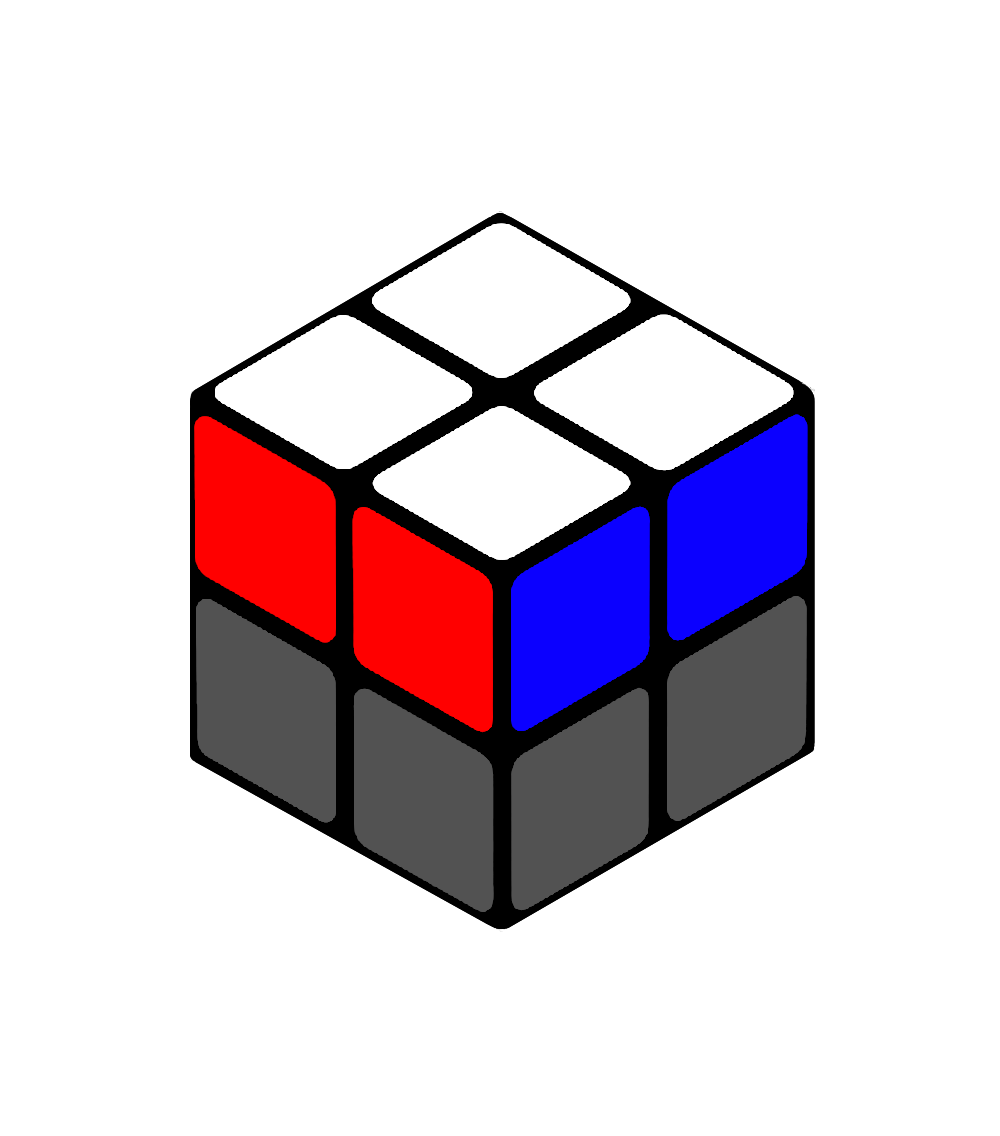
\includegraphics[scale=0.1]{ebene.png}
\caption[Ebene des Würfels]{Ebene des Würfels}
\label{24}
\end{figure}

\begin{center}
\begin{tabular}{cl}
\toprule
\textbf{Abkürzung} & \textbf{Beschreibung des Zugs} \\
\midrule
$U$ & Drehung der \textbf{oberen} Ebene im Uhrzeigersinn \\
$D$ & Drehung der \textbf{unteren} Ebene im Uhrzeigersinn \\
$R$ & Drehung der \textbf{rechten} Ebene im Uhrzeigersinn \\
$L$ & Drehung der \textbf{linken} Ebene im Uhrzeigersinn \\
$F$ & Drehung der \textbf{vorderen} Ebene im Uhrzeigersinn \\
$B$ & Drehung der \textbf{hinteren} Ebene im Uhrzeigersinn \\
\bottomrule
\end{tabular} 
\end{center}

Die Kürzel stehen für \textit{Up, Down, Right, Left, Front, Back}. 
Die entsprechende Ebene wird um $90^\circ$ im Uhrzeigersinn gedreht, wenn man auf diese Ebene schaut. Es wirkt also so, also würde man die untere Ebene gegen den Uhrzeigersinn drehen, wenn man von oben auf den Würfel schaut.  


Da der Würfel aber immer nur zwei nebeneinanderliegende Ebenen hat, entspricht eine Drehung der oberen Ebene nach rechts, einer Drehung der unteren Ebene nach links. 
Auf die Rotationsmöglichkeiten des kompletten Würfels wird im Verlauf dieser Arbeit noch eingegangen. Trotzdem werden die Drehungen für jede Ebene definiert. Das ist zwar nicht minimal, dient aber der besseren Anschaulichkeit und Übertragbarkeit der Algorithmen.
Sonst entspräche beispielsweise eine Drehung der oberen Ebene im Uhrzeigersinn ($U$) einer dreifachen Drehung der unteren Ebene im Uhrziegersinn ($DDD$) mit anschließender Rotation des kompletten Würfels. Es ist aber übersichtlicher, jede Ebenendrehung als einzelnen Zug darzustellen.

Die Ebenen werden bei einer Ebenendrehung um $90^\circ$ gedreht. Eine Ebenendrehung um $180^\circ$ wird als zwei Vierteldrehungen gewertet. Das nennt man \textit{Quarter-Turn} Metrik. Es gibt noch andere Metriken, wie z.B. die \textit{Half-Turn} Metrik, bei der eine Drehung der Ebene um $90^\circ$ oder um $180^\circ$ als eine Drehung gezählt werden. \cite{TR}


%
%
%
%
%
%
%
%
%=======================================================================================================
%
%
%
%
%
%
%
%
%


\newpage
\section{Mathematische Grundlagen}

In diesem Kapitel werden die mathematischen Grundlagen erklärt, die für den weiteren Inhalt dieser Arbeit relevant sind. Es wird die Definition einer Gruppe (auch anhand von Beispielen) und die der Untergruppen erklärt. Dazu werden auch Erzeuger (die Untergruppen erzeugen) und zyklische Gruppen definiert. Außerdem werden Permutationen und die Zykelschreibweise eingeführt und erklärt. 
Die genannten Definitionen basieren auf denen von Tobias Glosauer aus dem Buch \textit{Elementar(st)e Gruppentheorie} \cite{Buch}. Dort kann man auch detailliertere Informationen, Beispiele und weitere Definitionen nachlesen.
Des weiteren wird der Cayleygraph erklärt. 
%
%
%
%=======================================================================================================
%
%
%
\subsection*{Definition einer Gruppe} \addcontentsline{toc}{subsection}{\protect\numberline{}Definition einer Gruppe}


Die Definition einer Gruppe $(G, \circ)$ ist Grundlage für die folgenden Kapitel. 

\begin{singlespacing}
\begin{definition}[Gruppe]
Eine Menge $G$ (auch Trägermenge) mit einer Verknüpfung $\circ$ nennt man Gruppe, wenn diese Bedingungen gelten: 
\begin{itemize}
\item Abgeschlossenheit: $\forall a,b \in G.(a \circ b) \in G $
\item Assoziativität: $\forall a,b,c \in G.(a \circ b) \circ c = a \circ (b \circ c)$
\item Existenz eines neutralen Elements $n$: $\forall a \in G, \exists n \in G.n \circ a = a \circ n = a$ 
\item Existenz eines inversen Elements $a^{-1}$: $\forall a \in G, \exists a^{-1} \in G. a \circ a^{-1} = a^{-1} \circ a = n$ 
\end{itemize}
\end{definition}
\end{singlespacing}
Wenn es sich bei der Gruppe um eine kommutative Gruppe (auch abelsche Gruppe\footnote{\glqq Zu Ehren von Niels Henrik \textsc{Abel} (1802-1829); norwegischer Mathematiker und einer der Begründer der Gruppentheorie. Starb leider verarmt und deprimiert im Alter von 26 Jahren an Tuberkulose, kurz bevor er als Anerkennung für seine genialen Arbeiten  eine Dozentenstelle in Berlin angeboten bekam.\grqq \  \cite[S.21, Z.23]{Buch}}) handelt, muss zusätzlich noch die Eigenschaft der Kommutativität gelten: 
\begin{singlespacing}
\begin{definition}[Kommutative Gruppe]
Eine Gruppe $(G, \circ)$ ist eine kommutative Gruppe, wenn gilt:
\begin{itemize}
\item Kommutativität: $\forall a,b \in G.(a \circ b) = (b \circ a) $
\end{itemize}
\end{definition}
\end{singlespacing}

\textbf{Beispielgruppen}

Zur Veranschaulichung der Gruppendefinition werden hier die natürlichen Zahlen $\mathbb{N}$ und die ganzen Zahlen $\mathbb{Z}$ mit dem Operator $+$ auf die Gruppenaxiome untersucht.
\begin{itemize}
\item Die Abgeschlossenheit gilt sowohl für $(\mathbb{N},+)$ als auch für $(\mathbb{Z},+)$, da zwei natürliche Zahlen addiert immer eine natürliche Zahl ergeben. Zwei ganze Zahlen addiert ergeben immer eine ganze Zahl. \\
Beispielsweise sind $1+2=3$ und es gilt $1,2,3 \in \mathbb{N}$.
\item Die Verknüpfung ist assoziativ, da das Pluszeichen so definiert ist.
\item Das neutrale Element von $(\mathbb{N},+)$ und $(\mathbb{Z},+)$ ist $0$. Es gilt also $\forall n \in N. \ n + 0 = 0 + n = n$ (und mit $\mathbb{Z}$ analog). \\
Ein Beispiel zur Veranschaulichung: $3+0=0+3=3$
\item Die letzte erfordleriche Eigenschaft einer Gruppe ist die Existenz eines inversen Elements. Für die Gruppe $(\mathbb{Z},+)$ ist $-z$ das inverse Element für jedes $z \in \mathbb{Z}$. Für $(\mathbb{N},+)$ gibt es kein inverses Element.
\end{itemize}
Anhand der oberen Axiome kann man nun feststellen, dass $(\mathbb{Z},+)$ die Gruppeneigenschaften erfüllt, $(\mathbb{N},+)$ aber nicht. 
$(\mathbb{Z},+)$ ist also eine Gruppe und $(\mathbb{N},+)$ nicht, da kein inverses Element existiert. 
Es ist aber zu beachten, dass es sich hierbei nicht um formelle Beweise, sondern um anschauliche Beschreibungen handelt.
Nun kann man $(\mathbb{Z},+)$ noch auf die Kommutativität untersuchen, um zu prüfen, ob es sich um eine abelsche Gruppe handelt. \\
Da der Plus-Operator als kommutativ definiert ist, ist $(\mathbb{Z},+)$ eine abelsche Gruppe.

%
%
%
%
%
%=======================================================================================================
%
%
%
%
%
\subsection*{Untergruppen} \addcontentsline{toc}{subsection}{\protect\numberline{}Untergruppen}

Im Folgenden werden Untergruppen definiert.

\begin{singlespacing}
\begin{definition}[Untergruppe]
Eine Gruppe $(H, \circ)$ ist eine Untergruppe einer Gruppe $(G, \circ)$, wenn $H \subseteq G$ gilt. Dann schreibt man auch $H \leqslant G$. 
\end{definition}
\end{singlespacing}
Das Symbol $\leqslant$ ist zu lesen als \textit{ist Untergruppe von}. Nicht jede Teilmenge $H \subseteq G$ muss auch eine Gruppe sein.

Wenn $(H, \circ)$ eine Untergruppe der Gruppe $(G, \circ)$ ist, so nennt man $(G, \circ)$ auch eine Obergruppe von $(H, \circ)$.
Jede Gruppe G mit neutralem Element $N$ hat die beiden trivialen Untergruppen ${H_N = \{N\}}$ und $H_G=G$.


\textbf{Beispieluntergruppe}

Bei dem oben genannten Beispiel mit $(\mathbb{N},+)$ und $(\mathbb{Z},+)$ stellte sich heraus, dass $(\mathbb{Z},+)$ eine Gruppe ist und $(\mathbb{N},+)$ nicht. Obwohl $\mathbb{N \subseteq \mathbb{Z}}$, ist $(\mathbb{N},+)$ \textit{keine} Untergruppe von $(\mathbb{Z},+)$, da die Gruppeneigenschaft \textit{Existenz eines inversen Elements} nicht erfüllt sind.
%
%
%
%
%
%=======================================================================================================
%
%
%
%
%

\subsection*{Erzeuger und zyklische Gruppe} \addcontentsline{toc}{subsection}{\protect\numberline{}Erzeuger und zyklische Gruppe}


\begin{singlespacing}
\begin{definition}[Erzeuger]
Sei die Menge $M \subseteq G$ eine nicht leere Teilmenge der Trägermenge einer Gruppe $(G, \circ)$. 
Dann wird die Untergruppe $(M, \circ)$ von $M$ erzeugt und ist die kleinste Untergruppe von $(G, \circ)$, für die $M \subseteq G$ gilt.
Man nennt $(M, \circ)$ dann das Erzeugnis von $M$ und die Elemente aus $M$ sind die Erzeuger der Untergruppe $(M, \circ)$.
\end{definition}
\end{singlespacing}
Wenn $(M, \circ)$ durch $M$ erzeugt wird, ist dann eine $M$ enthaltende Untergruppe.

Eine zyklische Gruppe ist eine Gruppe, die von nur einem Element erzeugt wird. Sie besteht also nur aus Potenzen dieses Elementes
\begin{singlespacing}
\begin{definition}[Zyklische Gruppe]
Sei $(G, \circ)$ eine Gruppe. $(G, \circ)$ nennt man eine zyklische Gruppe, wenn sie ein Element $a \in G$ gibt, das jedes Element in $G$ erzeugt. Dann schreibt man auch:
\begin{align*}
\langle a \rangle := \{ a^n \mid n \in \mathbb{Z} \}
\end{align*}

\end{definition}
\end{singlespacing}


Ein Beispiel für Erzeuger findet man anhand der Gruppe der ganzen Zahlen $(\mathbb{Z},+)$ und der Addition als Verknüpfung, die bereits als Beispiel der Gruppe beschrieben wurde.

Die Operationen sind hier die Addition und der Übergang von einer Zahl $z$ zu der negativen Zahl $-z$.

Ein Erzeuger dieser Gruppe ist die einelementige Menge $M = \{ 1 \}$. Jede positive Zahl $n$ lässt sich durch die $n$-fache Addition von $1$ erzeugen und jede negative Zahl durch  die Addition von $((-1)+(-1)...)$. Man kann den Erzeuger der zyklischen Gruppe auch als $\langle 1 \rangle$ schreiben.
%
%
%
%
%=======================================================================================================
%
%
%
%
%
\subsection*{Cayleygraph} \addcontentsline{toc}{subsection}{\protect\numberline{}Cayleygraph}
Ein Cayleygraph ist ein Graph, der die Struktur einer Gruppe beschreibt. Er hängt von der Menge der Erzeuger ab und dient dazu, Gruppen bildlich darzustellen.
Es handelt sich dabei um einen Graphen mit Knoten, die die verschiedenen Gruppenelemente darstellen. Pfeile zeigen von einem Element zum nächsten, wenn dies durch einen der Erzeuger erreicht werden kann. \cite{AT}

%
%
%
%
%=======================================================================================================
%
%
%
%
%
%

\subsection*{Gruppenoperation} \addcontentsline{toc}{subsection}{\protect\numberline{}Gruppenoperation}

Es gibt Links- und Rechtsoperationen auf Gruppen. Da im Folgenden nur Rechtsoperationen genutzt werden, werden auch nur diese hier definiert.

\begin{singlespacing}
\begin{definition}[Rechtsoperation]

Eine Rechtsoperation einer Gruppe $(G, *)$ auf einer Menge $M$ ist eine Verknüpfung mit $m \in M$, $e$ als neutralem Element von $G$ und $g,h \in G$:
\begin{align*}
\cdot: M \times G \rightarrow M \ \ \ \ \ \ \ \ \ \ \ \ \ \ \
(m, g) \mapsto m \cdot g 
\end{align*}
Die folgenden beiden Eigenschaften müssen gelten:
\begin{align*}
m \cdot e & = m \\
n \cdot (g * h) & = (n \cdot g) \cdot h
\end{align*}
Dann operiert $G$ von rechts auf $M$.

\end{definition}
\end{singlespacing}
%
%
%
%
%
%=======================================================================================================
%
%
%
%
%
%
%

\subsection*{Kommutator} \addcontentsline{toc}{subsection}{\protect\numberline{}Kommutator
}
Ein Kommutator misst, wie sehr eine Gruppe das Kommutativgesetz verletzt. 
\begin{singlespacing}
\begin{definition}[Kommutator]
Als Kommutator von zwei Elementen $a, b$ einer Gruppe $(G, \circ)$  bezeichnet man $[a,b] = aba^{-1}b^{-1}$.
\end{definition}
\end{singlespacing}
Bei kommutativen Gruppen ist der Kommutator zweier Elemente das neutrale Element der Gruppe \cite{TD}. Man sagt dann, dass die beiden Elemente kommutieren. 


%
%
%
%
%
%
%=======================================================================================================
%
%
%
%
%
%
%

\subsection*{Äquivalenzrelation} \addcontentsline{toc}{subsection}{\protect\numberline{}Äquivalenzrelation}

Mit Relationen lassen sich Beziehungen von Elementen einer Menge zueinander beschreiben.
\begin{singlespacing}
\begin{definition}[Äquivalenzrelation]
Eine Relation $R \subseteq A \times A$ heißt Äquivalenzrelation auf $A$, wenn für alle $x, y, z \in A$ die drei folgenden Eigenschaften gelten: Reflexivität, Symmetrie, Transitivität.
\end{definition}
\end{singlespacing}

Hier liest man $x \sim y$ als \textit{x ist äquivalent zu y}. Im Folgenden werden noch die Bedeutungen von Reflexivität, Symmetrie und Transitivität aufgelistet:

\begin{center}
\begin{tabular}{ll}
$x \sim x$ & (Reflexivität) \\
Aus $(x \sim y)$ folgt $(y \sim x)$. & (Symmetrie) \\
Aus $(x \sim y)$ und $(y \sim z)$ folgt $(x \sim y)$. & (Transitivität) \\
\end{tabular}
\end{center}


\textbf{Beispieläquivalenzrelation:}

Für die Menge $A=\{ 1, 2, 3, 4, 5 \}$ werden nun zwei verschiedene Relationen betrachtet:
\begin{itemize}
\item $x \sim_< y :\Leftrightarrow x < y$

Bei der Relation $\sim_< $ handelt es sich nicht um eine Äquivalenrelation, da die Eigenschaft der Reflexivität nicht gilt: $1 \nless 1$. Auch die Symmetrie gilt nicht.
\item $x \sim_= y :\Leftrightarrow x = y$

Bei der Relation $\sim_=$ gilt die Reflexivität für alle Elemente, da die Gleichheit reflexiv ist. Auch die Symmetrie und die Transitivität gelten für die Gleichheit und $\sim_=$ ist ja als Gleichheit definiert. 
\end{itemize}


%
%
%
%
%
%
%=======================================================================================================
%
%
%
%
%
%
%
\subsection*{Permutationen und Zykelschreibweise} \addcontentsline{toc}{subsection}{\protect\numberline{}Permutationen und Zykelschreibweise}
\label{11}
Unter einer Permutation versteht man die Reihenfolge von Objekte. Bei einer $n$-elementigen Menge $M$ ist eine ($n$-stellige) Permutation ist eine bijektive Abbildung $f: M \rightarrow M$. Die Zykelschreibweise ist eine kurze Schreibweise für eine Permutation.
Permutationen und die Zykelschreibweise werden anhand eines Beispiels erklärt: 

Man hat fünf Objekte: $1, 2, 3, 4$ und $5$. Nun kann man diese Objekte in fünf Plätzen arrangieren. Die Plätze werden als $1$ bis $5$ nummeriert. Dann kann man eine Funktion $f:\{1,2,3,4,5\} \rightarrow \{1,2,3,4,5\}$ definieren, bei der $f(i)$ die Zahl ist, die in Slot $i$ liegt.
Wenn man die Zahlen in der Reihenfolge $5 \ 1\ 4\ 3 \ 2$ anordnet, ist $5$ auf Platz $1$, $1$ auf Platz $2$, usw. Das sieht man auch in der folgenden Tabelle: 

\begin{center}
\begin{tabular}{l ccccc}

Platz & 1 & 2 & 3 & 4 & 5 \\
\midrule
Zahl & 5 & 1 & 4 & 3 & 2 \\

\end{tabular}
\end{center}

Die Funktion $f$ sieht für diese Permutation (s. Tabelle) also so aus:
\begin{align*}
f(1) = 5 \ \ \ \ \ \  f(2) = 1 \ \ \ \ \ \ f(3) = 4 \ \ \ \ \ \ f(4) = 3 \ \ \ \ \ \ f(5) = 2 
\end{align*}
Man kann $f$ auch als eindeutige Zuordnung der Form $i \mapsto j$ schreiben (für $f(i)=j$) \cite{JC}:
\begin{align*}
1 \mapsto 5 \ \ \ \ \ \ \ \ \ \  2\mapsto 1 \ \ \ \ \ \ \ \ \ \ 3\mapsto 4 \ \ \ \ \ \ \ \ \ \ 4\mapsto 3 \ \ \ \ \ \ \ \ \ \ 5\mapsto 2 
\end{align*}
Das kann man auch in der Zykelschreibweise schreiben:
\begin{align*}
f = (1 \ 5 \ 2)\ (3 \ 4)
\end{align*}
Das liest man so: Die 1 geht auf die 5, die 5 geht auf die 2, die 2 geht wieder auf die 1. Damit ist der erste Zykel geschlossen. Beim zweiten Zykel geht die 3 auf die 4 und die 4 auf die 3. Man sagt, dass $f$ aus zwei Zykeln besteht: ein Zykel hat die Länge drei und der andere die Länge zwei. Die Zykel kann man auch in Abbildung \ref{10} sehen.
\begin{figure}[h]
\centering
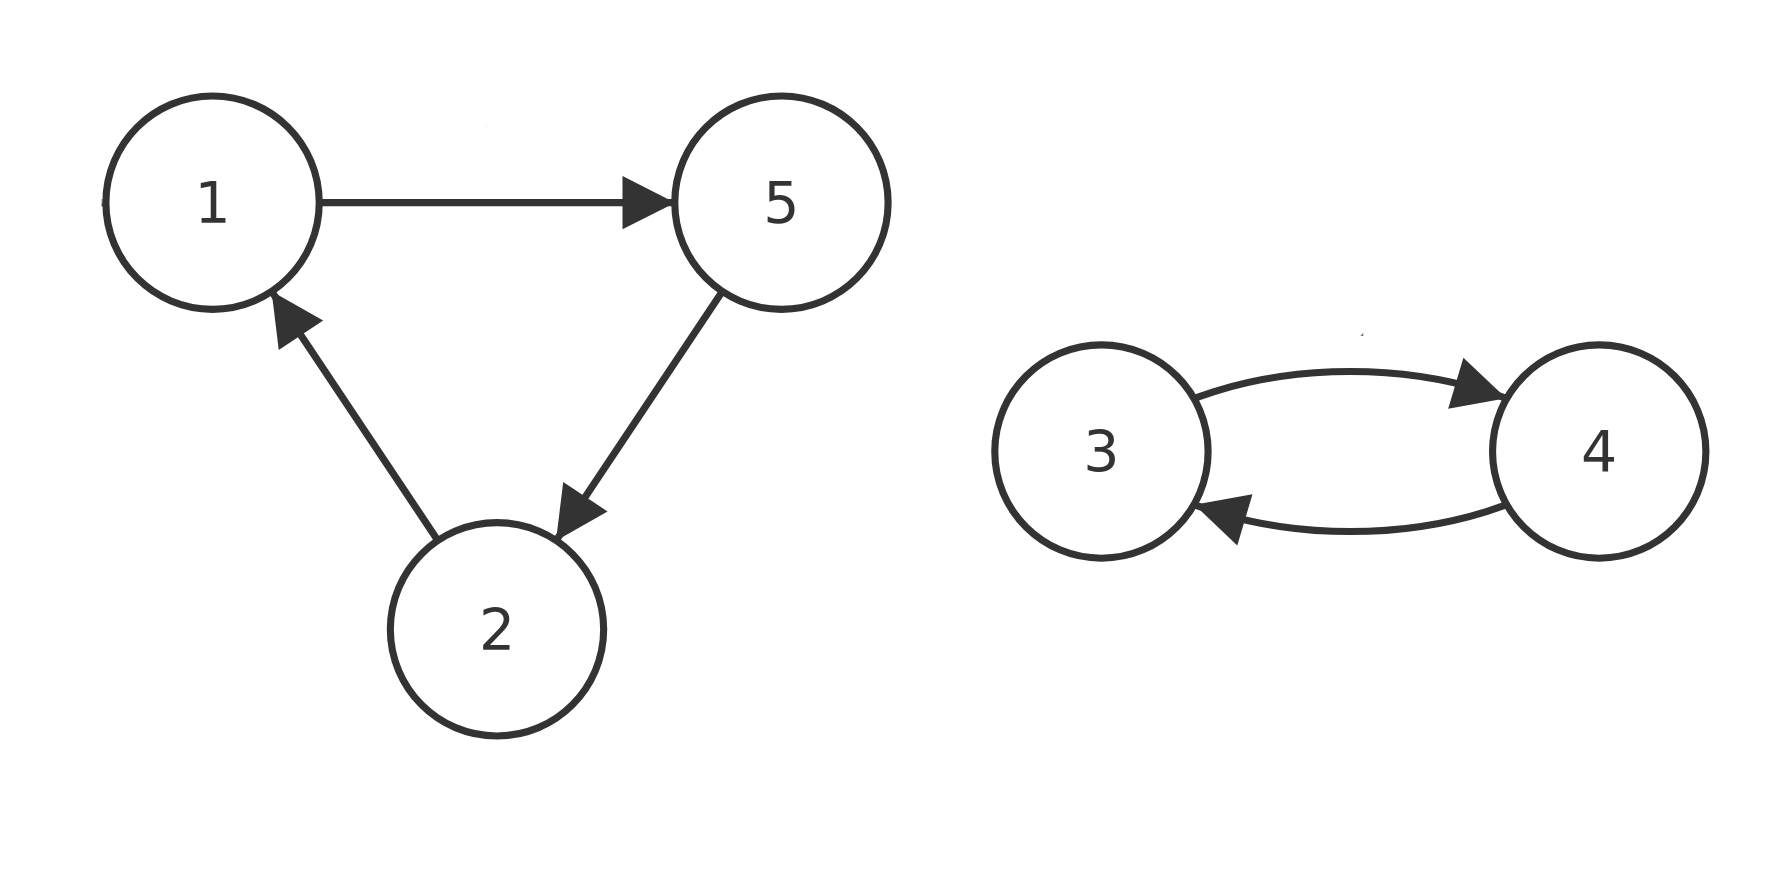
\includegraphics[scale=0.13]{Zykel_152.png}
\caption{Zykel $f = (1 \ 5 \ 2)\ (3 \ 4)$}
\label{10}
\end{figure}
Wichtig bei der Zykelschreibweise ist die Reihenfolge der Elemente. Beispielsweise ist $(1 \ 2 \ 3)$ nicht das gleiche wie $(1 \ 3 \ 2)$. Wenn die Reihenfolge bestehen bleibt, können die Zykel aber bei jedem beliebigen Element beginnen. Es gilt in dem Beispiel $(1 \ 2 \ 3)$ also $(1 \ 2 \ 3) = (2 \ 3 \ 1) = (3\ 1 \ 2 \ )$.


%
%
%
%
%=======================================================================================================
%
%
%
%
%
%
\newpage

\section{Konfiguration des Würfels}

\label{26}
Um mit dem Würfel zu arbeiten, muss man wissen, in welcher Position er sich befindet.
Deshalb wird die Konfiguration des Würfels definiert, bevor der Würfel als Gruppe dargestellt wird. Die Würfelkonfiguration setzt sich aus zwei Parametern zusammen: 
\begin{itemize}
\item Position der Ecksteine (angegeben als $\sigma$)
\item Ausrichtung der Ecksteine (angegeben als $x$)
\end{itemize}
Also kann die Konfiguration des Würfels als ein 2-Tupel geschrieben werden: $(\sigma, x)$.
In diesem Kapitel wird die Position derEcksteine als $\sigma$ und die Ausrichtung der Ecktsteine als Vaktor $x$ erklärt. 
Außerdem werden Äquivalenzrelationen definiert, um die Ausrichtung des Würfels zu berücksichtigen.

%
%
%
%
%
%
%
%
%
%
%=======================================================================================================
%
%
%
%
%
%
%
%
%
%
\subsection*{Positionen der Steine im Würfel} \addcontentsline{toc}{subsection}{\protect\numberline{}Positionen der Steine im Würfel}

Die bijektive Funktion $\sigma$ (für jede Ebenenrotation) stellt Übergänge der Würfelsteine als Funktion dar. Die Übergänge beschreiben die Positionsänderung der Steine bei einem Zug. $\sigma$ bildet jede der Würfelpositionen auf die neue Position ab. Es handelt sich dabei um eine Permutation. Permutationen wurden in Kapitel \ref{11} erklärt. 

Die Einteilung der Würfelpositionen sieht man in den Abbildung \ref{13} und \ref{14}. Die einzelnen Steinpositionen werden mit den Kürzeln benannt, die \textit{up, down, left, right, front und back} beschreiben.
\begin{figure}[h]
\centering
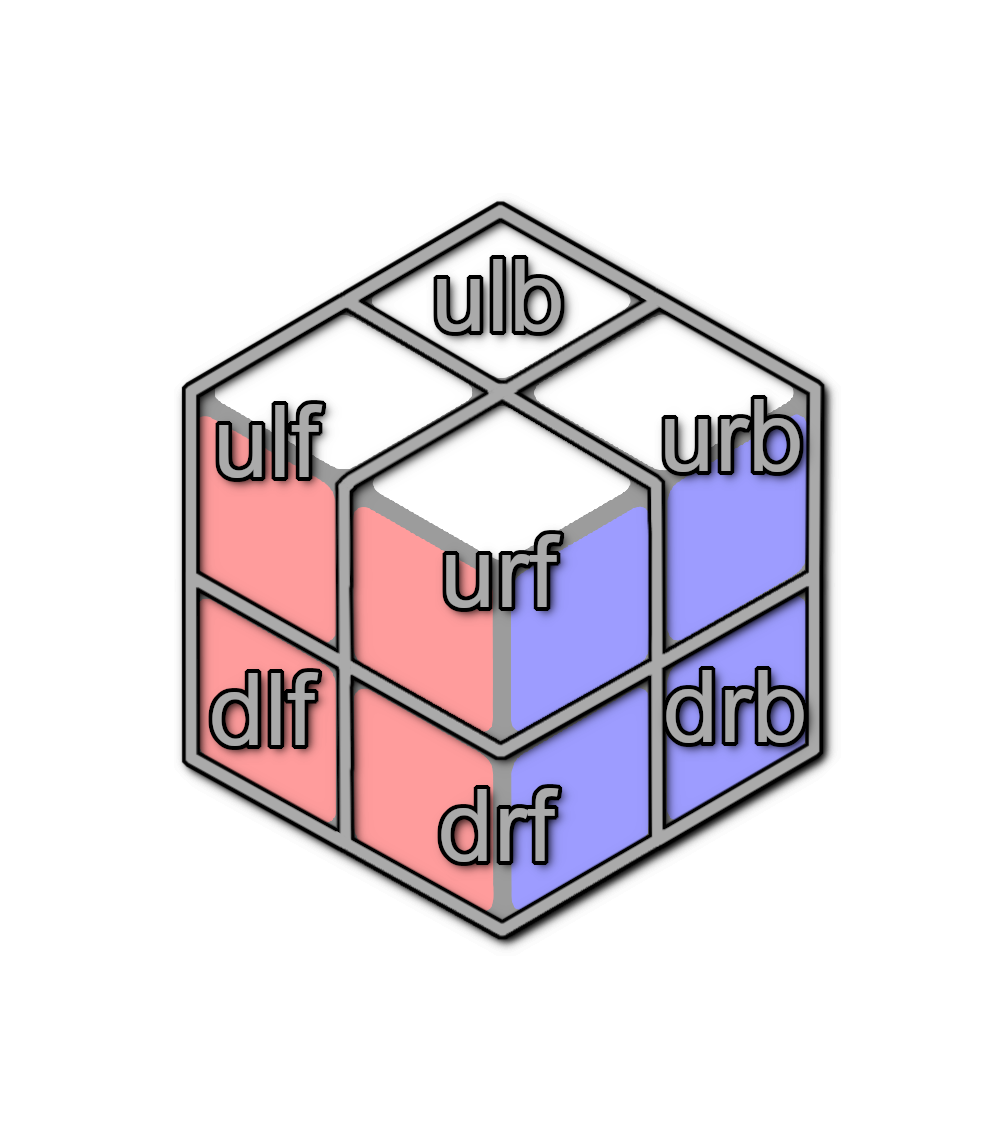
\includegraphics[scale=0.15]{caged_positions.png} \\
\caption[Namen der Steinpositionen im Würfel]{Namen der Steinpositionen im Würfel}
\label{13}
\end{figure}

\begin{figure}[h]
\centering
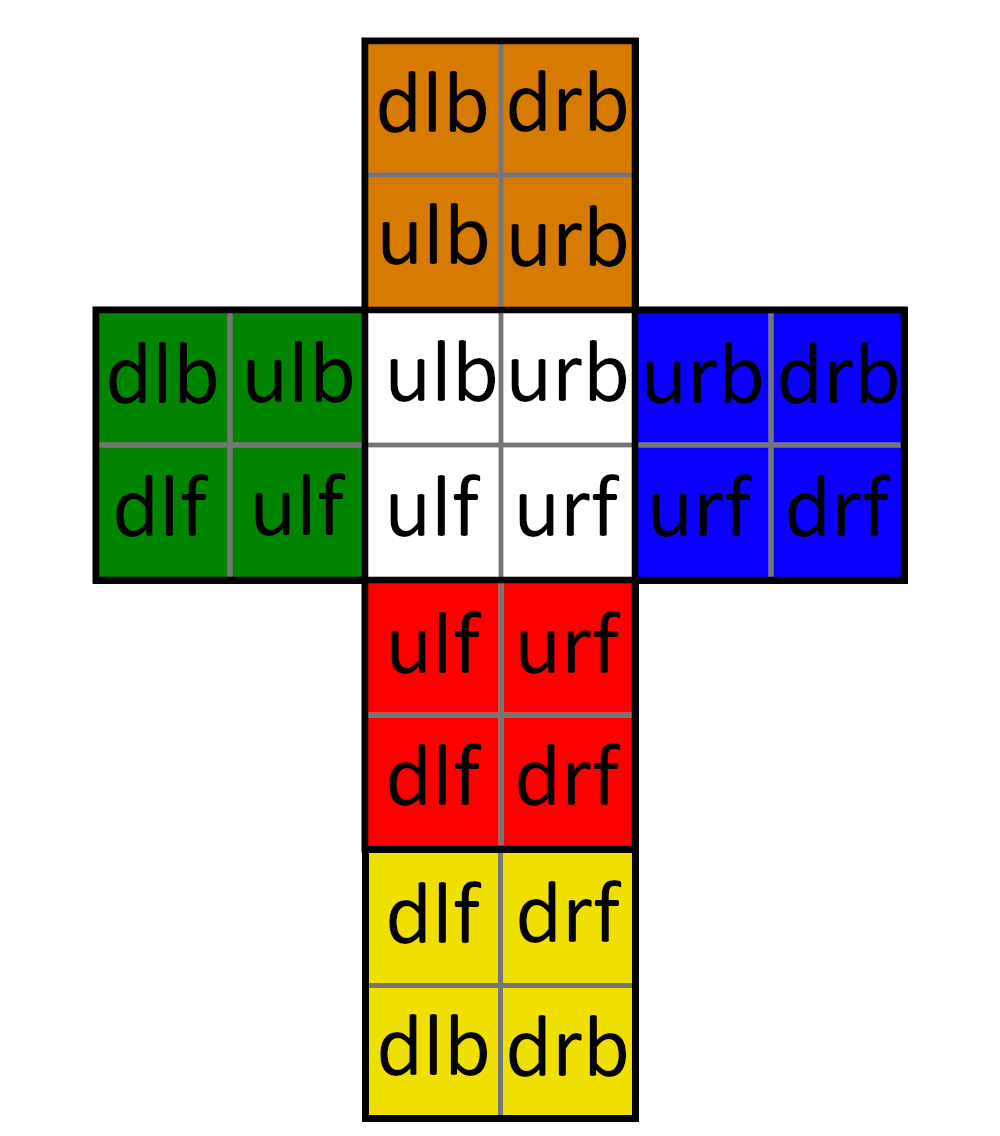
\includegraphics[scale=0.15]{foldedout_cage.png}
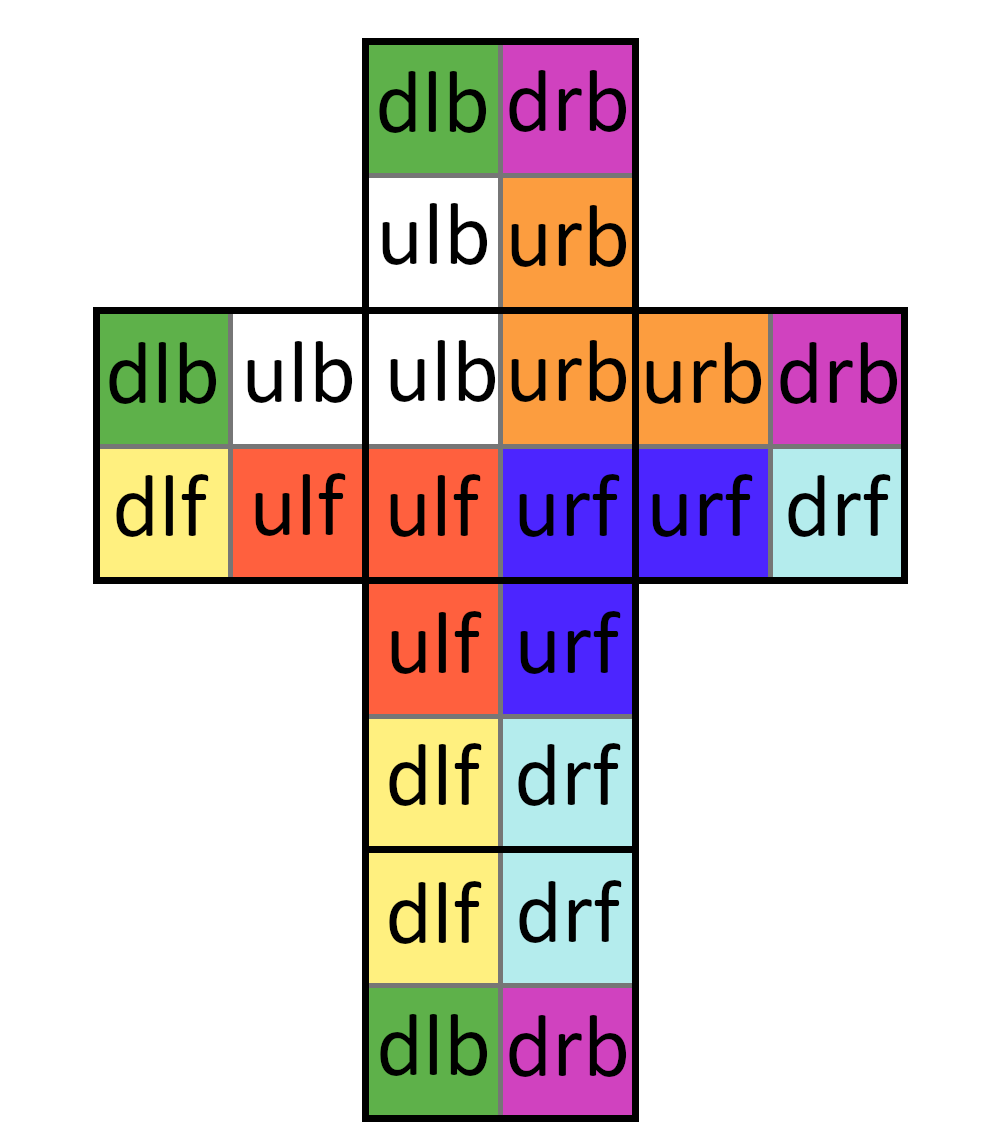
\includegraphics[scale=0.15]{foldedout_cage_color.png}
\caption[aufgeklappter Würfel mit Namen der Steinpositionen]{aufgeklappter Würfel mit Namen der Steinpositionen}
\label{14}
\end{figure}
Jeder Steinposition wird ein einzigartiger Name zugeordnet, um sich darauf zu beziehen. Dabei wird davon ausgegangen, dass die weiße Seite in der Startkonfiguration oben ist und die rote Seite vorne. Die Steinposition werden mit 3 Buchstaben beschrieben, die aus den Kürzeln \textit{u, d, l, r, f, b} bestehen. Diese Kürzel stehen für \textit{up, down, left, right, front, back}. \\
Somit heißt die Steinposition oben links beispielsweise \textit{ulf} (für \textit{up}, \textit{left} und \textit{front}). 
Jeder Stein bekommt auch einen eindeutigen Namen, der seiner Steinposition im gelösten Zustand entspricht. Beispielsweise liegt der Stein \textit{ulf} im gelösten Zustand an der Steinposition \textit{ulf}.

Nun wird zur Veranschaulichung die Permutation $\sigma_U$ für eine Drehung der oberen Ebene um 90$^\circ$ im Uhrzeigersinn definiert. Grundlagen zu Permutationen und der Zykelschreibeweise wurden in Kapitel \ref{11} erklärt.
Hier wird $\sigma_U$ ausführlich beschrieben und verschiedene Schreibweisen angegeben. Die weiteren Drehungen sind analog definiert. 
Die Drehung der oberen Ebene sieht man grafisch dargestellt in Abbildung \ref{15}.
\begin{figure}[h]
\centering
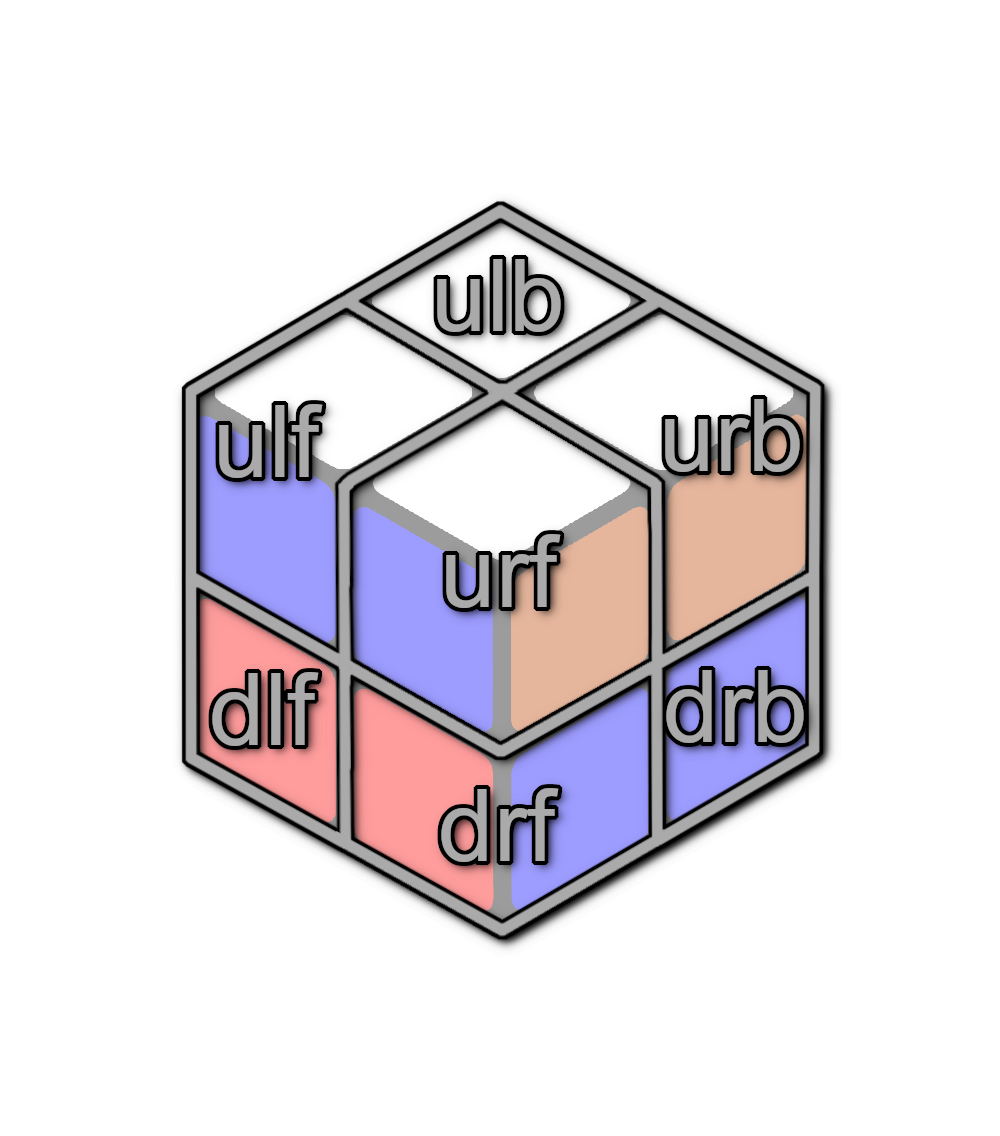
\includegraphics[scale=0.13]{caged_spin.png}
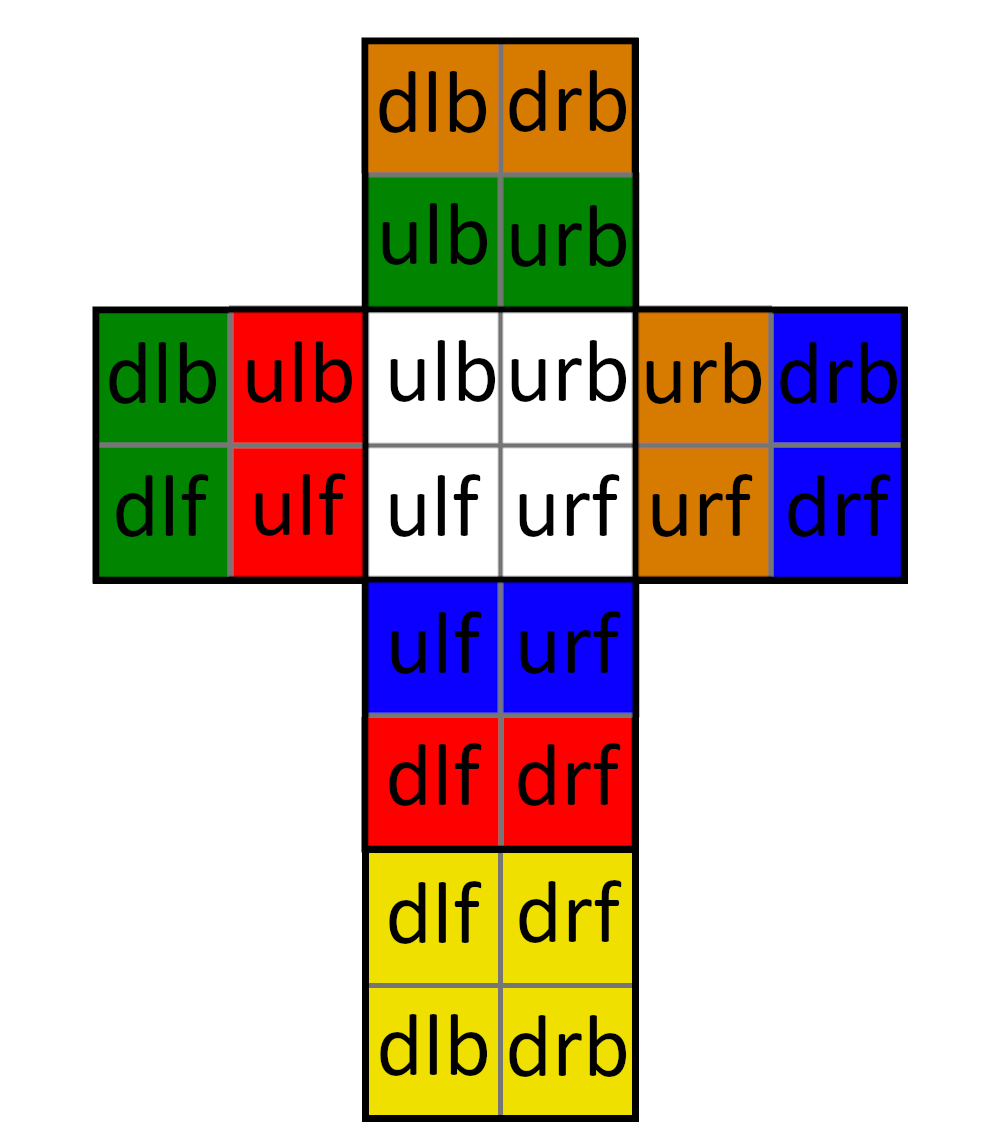
\includegraphics[scale=0.13]{foldedout_spin.png}
\caption[Steinpositionen nach Zug $U$]{Steinpositionen nach Zug $U$}
\label{15}
\end{figure}

Die Funktion $\sigma_U$ sieht dann so aus:
\begin{align*}
\sigma_U(ulf)=ulb \ \ \ \ \ \ \ \ \sigma_U(ulb)=urb \ \ \ \ \ \ \ \ \sigma_U(urb)=urf \ \ \ \ \ \ \ \ \sigma_U(urf)=ulf \\
\sigma_U(dlf)=dlf \ \ \ \ \ \ \ \ \sigma_U(dlb)=dlb \ \ \ \ \ \ \ \ \ \sigma_U(drb)=drb \ \ \ \ \ \ \ \ \sigma_U(drf)=drf 
\end{align*}

Das kann man auch in der Form $i \mapsto j$ schreiben: 
\begin{align*}
ulf \mapsto ulb \ \ \ \ \ \ \ \ ulb \mapsto urb \ \ \ \ \ \ \ \ urb \mapsto urf \ \ \ \ \ \ \ \ urf \mapsto ulf \\
dlf \mapsto dlf \ \ \ \ \ \ \ \ dlb \mapsto dlb \ \ \ \ \ \ \ \ \ drb \mapsto drb \ \ \ \ \ \ \ \ drf \mapsto drf 
\end{align*}

Daraus entstehen folgende Zykel: $\sigma_U = \ (ulf \ ulb \ urb \ urf)\ (dlf)\ (dlb)\ (drb)\ (drf)$

Die Zykel mit nur einem Element müssen nicht aufgeschrieben werden. Dann ergibt sich $\sigma_U = \ (ulf \ ulb \ urb \ urf)$, was den Zykel beschreibt, in dem die Steine rotiert werden, wenn die obere Ebene gedreht wird. 


Die Drehungen aller Ebenen können durch folgende Zykel beschrieben werden: 
\begin{align*}
\sigma_U & =\ (ulf \ ulb \ urb \ urf) \\
\sigma_D & =\ (dlf \ drf \ drb \ dlb) \\
\sigma_F & =\ (ulf \ urf \ drf \ dlf) \\
\sigma_B & =\ (ulb \ dlb \ drb \ urb) \\
\sigma_L & =\ (ulb \ ulf \ dlf \ dlb) \\
\sigma_R & =\ (urb \ drb \ drf \ urf) \\
\end{align*}

%
%
%
%
%
%
%
%
%
%
%=======================================================================================================
%
%
%
%
%
%
%
%
%
%
\subsection*{Ausrichtung der Steine} \addcontentsline{toc}{subsection}{\protect\numberline{}Ausrichtung der Steine}
Der $2\times 2\times 2$-Würfel besteht aus 8 Ecksteinen, die jeweils 3 Farbflächen haben. Somit hat jeder Stein 3 mögliche Ausrichtungen. 
Um die Ausrichtung der Steine zu erkennen, bekommen die Würfelpositionen an einer Farbfläche einer Nummer zugeordnet. Dafür werden die weißen und die gelben Seiten markiert und nummeriert. Auf diese Nummern wird sich als $x_i \in \lbrace 1, 2, 3, 4, 5, 6, 7, 8 \rbrace$ bezogen - mit $x_1$ als Position 1, $x_2$ als Position 2, usw.
\begin{figure}[h]
\centering
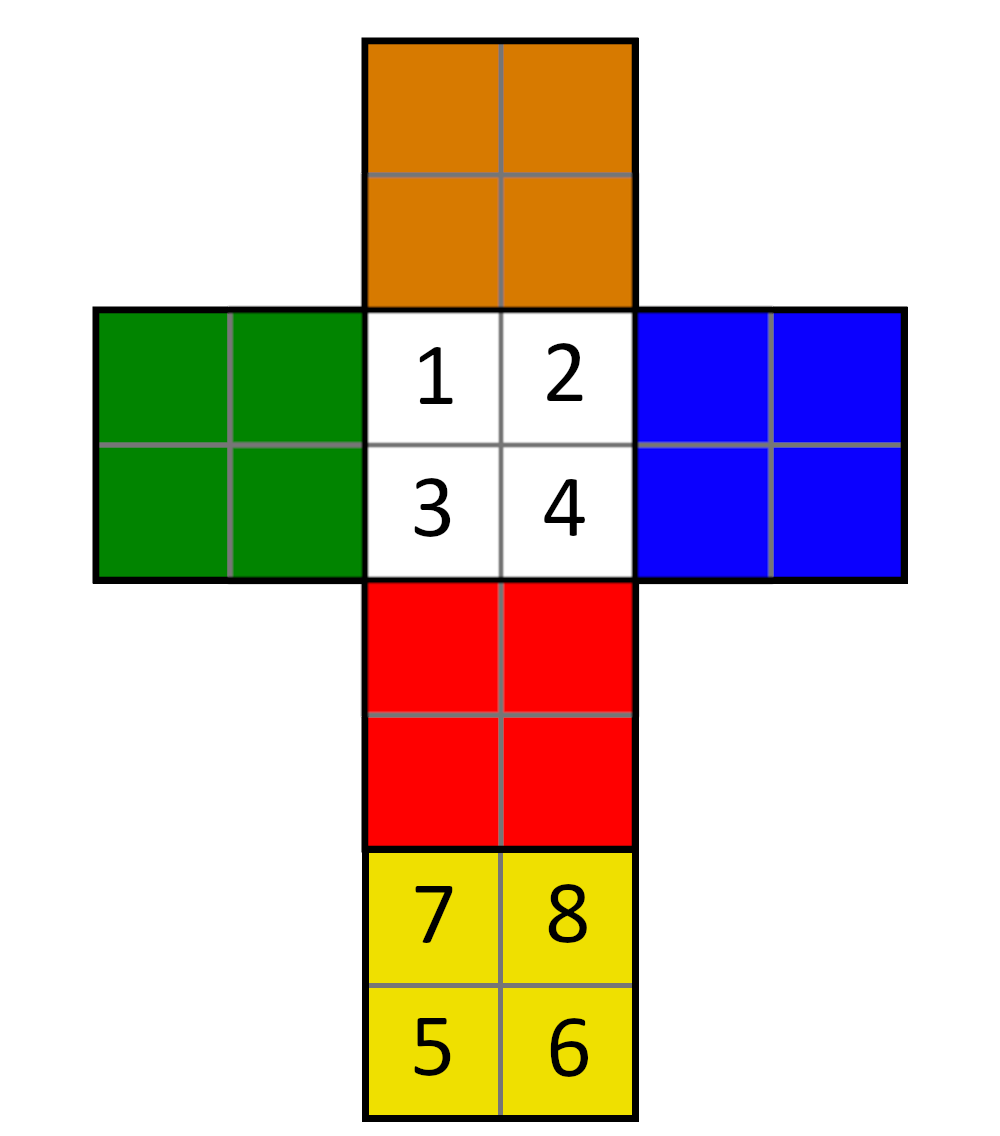
\includegraphics[scale=0.1]{foldedout_numbers.png}
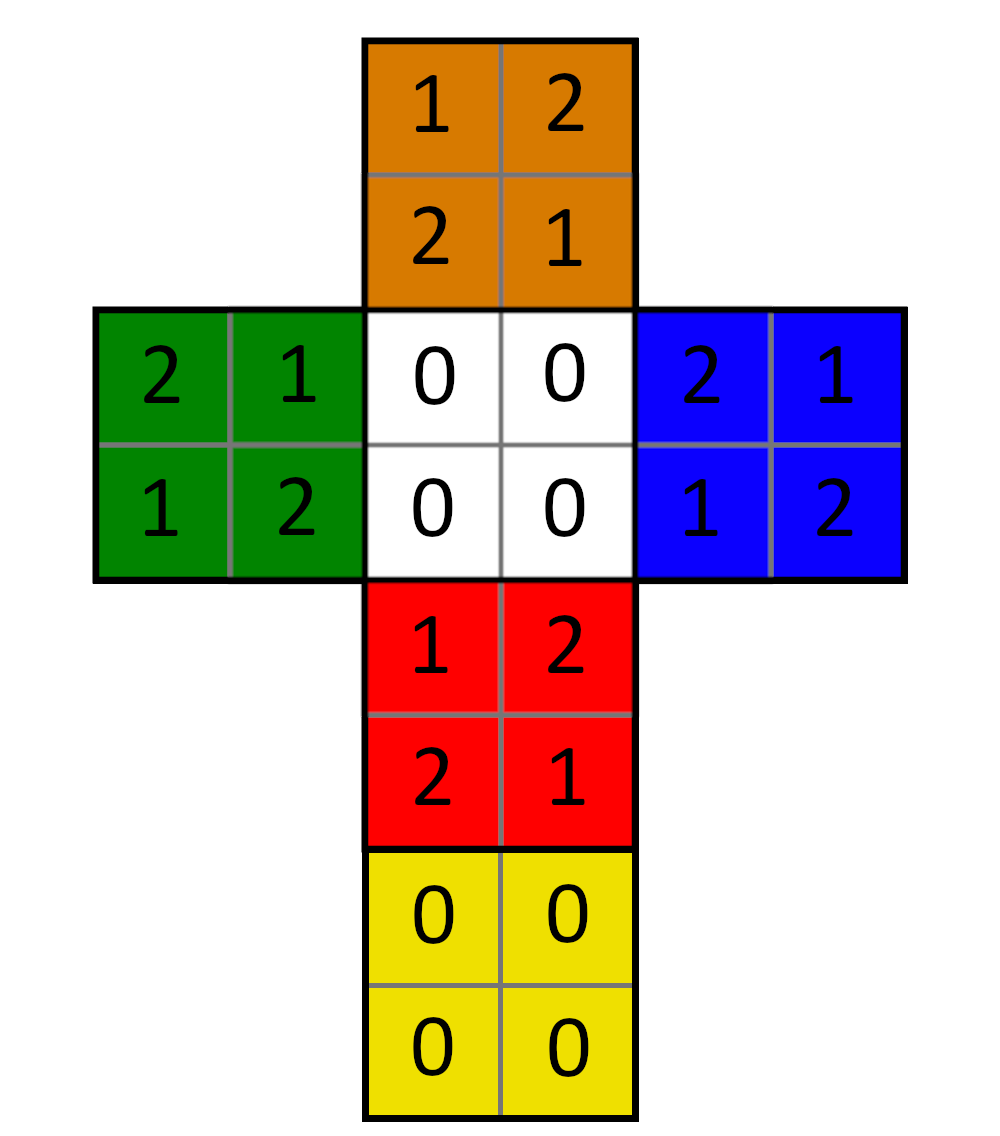
\includegraphics[scale=0.1]{foldedout_012.png}
\caption[Markierungen $x_i$ (links), Farbflächennummern (rechts)]{ausgeklappter Würfel mit Markierungen für $x_i$ (links) und Farbflächennummerierungen (rechts) }
\end{figure}
Außerdem bekommt jeder Stein an jeder Farbfläche eine Zahlenzuordnung. Da jeder Stein 3 Ausrichtungen haben kann, wird mit 0, 1 und 2 nummeriert. Die Nummerierung beginnt mit der weißen/gelben Fläche bei 0 und zählt dann im Uhrzeigersinn die Flächen. 
In der Startkonfiguration sind alle $x_i = 0$, der Vektor $x$ ist dann $(0, 0, 0, 0, 0, 0, 0, 0)$. Das wird kurz als $x=0$ geschrieben.

Nun wird der Zug $R$ als Beispiel ausgeführt (s. Abbildung \ref{7}) und die Veränderung der Nummerierung der Farbflächen dargestellt. $R$ ist eine Rotation der rechten Ebene um 90$^\circ$ im Uhrzeigersinn. 
Die Kennzeichnungen $x_{1-8}$ bleiben an der gleichen Position, die Nummerierungen  der Farbflächen ändern sich mit Rotation der Ebene und ermöglichen so eine Zuordnung der Ausrichtung der Ecksteine. 
Die linke Seite der Würfels wird dabei nicht beeinflusst, also sind die Flächen an den Positionen $x_1, x_3, x_5, x_7$ alle 0. 
Die anderen Positionen haben nun aber andere Farbflächen: 
\begin{align*}
x_2 = 2 \ \ \ \ x_4 = 1 \ \ \ \ x_6 = 1 \ \ \ \ x_8 = 2  
\end{align*}
Also gilt $x = (0, 2, 0, 1, 0, 1, 0, 2)$ nach dem Zug $R$. 
\begin{figure}[h]
\centering
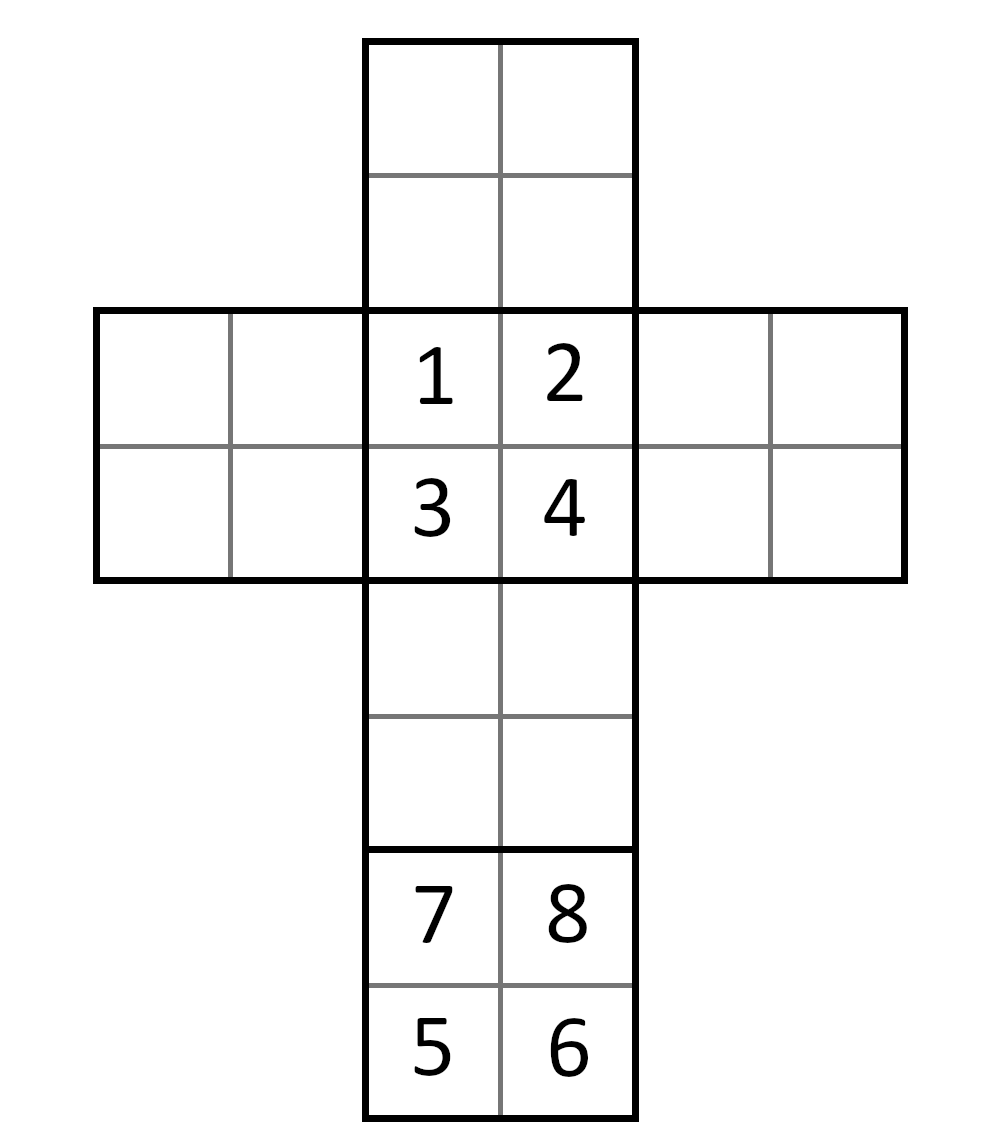
\includegraphics[scale=0.1]{foldedout_012_white.png}
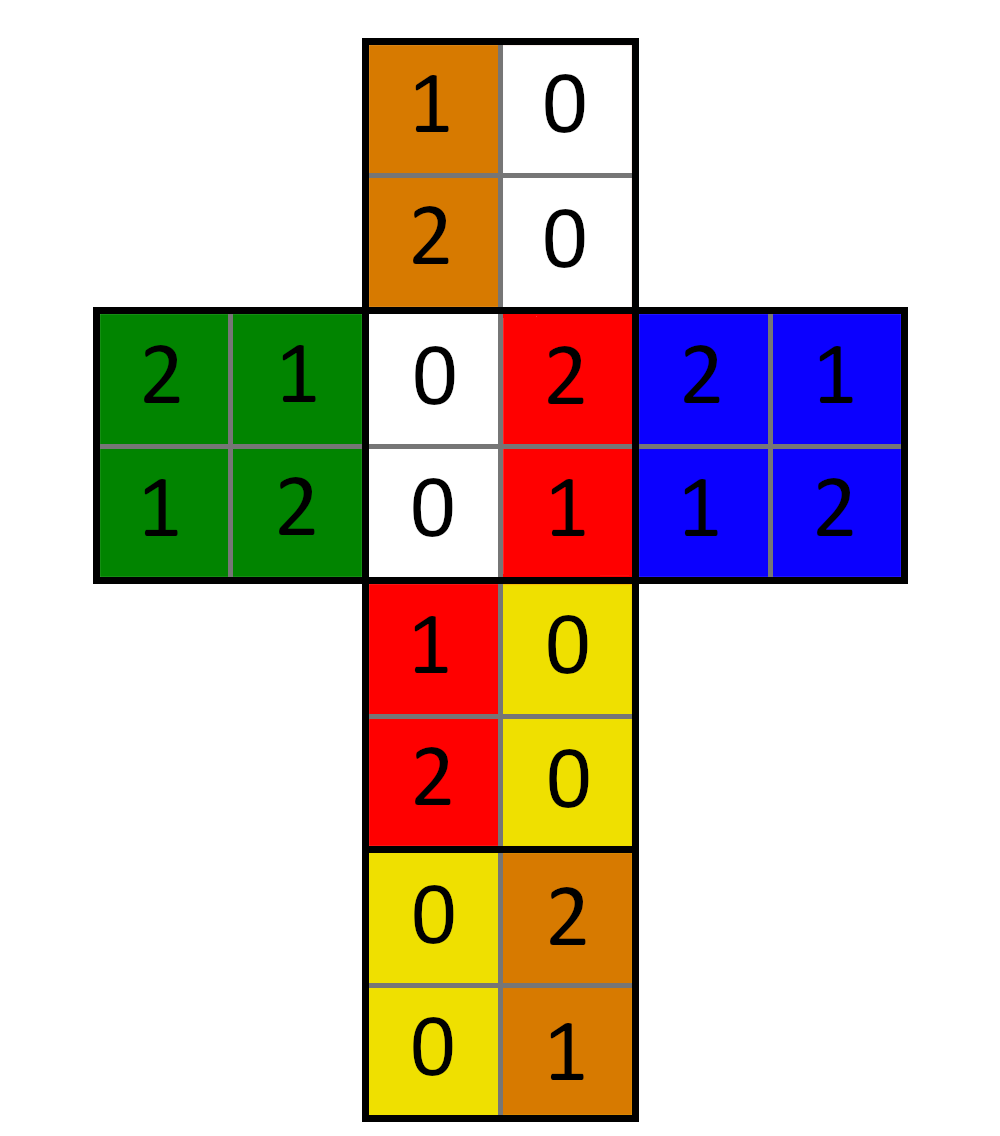
\includegraphics[scale=0.1]{foldedout_012_spin.png}
\caption[links: Positionen $x_1$ bis $x_8$, rechts: Veränderung der nummerierten Ecksteine nach dem Zug $R$]{links: Positionen $x_1$ bis $x_8$, rechts: Veränderung der nummerierten Ecksteine nach dem Zug $R$}
\label{7}
\end{figure}

%
%
%
%
%=======================================================================================================
%
%
%
%
%
%
\newpage
\section{Würfel als Gruppe}

In diesem Kapitel wird die Gruppe des \Tthree \textit{Cubes} auf den \Ttwo \textit{Cube} übertragen. Die Gruppe des \Ttwo Würfels wird auf die vier Gruppenaxiome (Abgeschlossenheit, Assoziativität, Existenz eines neutralen Elements und Existenz eines inversen Elements) untersucht und auf Kommutativität untersucht.

%
%
%
%
%=======================================================================================================
%
%
%
%
%
%

\subsection*{\Ttwo Zauberwüfel als Gruppe} \addcontentsline{toc}{subsection}{\protect\numberline{}\Ttwo Zauberwüfel als Gruppe}
\label{8}

Im Folgenden wird die Definition der Gruppe des \Tthree Würfels aus dem Paper \textit{Group Theory and the Rubik's Cube}  von Janet Chen \cite{JC} als Gruppe des \Ttwo Würfels umgesetzt. Die Gruppe von Janet Chen wird hier als $(\Gthree, *)$ bezeichnet, auch wenn er sie als $(G, *)$ bezeichnet hat. Der Namen der Gruppe wird geändert, um klar zwischen dem \Ttwo  und dem \Tthree Würfel zu differenzieren. Die Gruppe des \Ttwo Würfels heißt $(\Gtwo, \circ)$. 
Die Grundlagen und Definition der Gruppe wurden in Kapitel \ref{11} erklärt.


Die Menge $\Gtwo$ besteht aus allen möglichen Zügen des Würfels. Beispielsweise die Drehung der oberen Ebene ist ein Zug. Ein Zug kann aber auch aus mehreren Drehungen bestehen, z.B. das Drehen der oberen Ebene, gefolgt von dem Drehen der rechten Ebene stellt ebenfalls einen Zug dar. 
Wenn zwei Züge mit nach gleicher Ausgangsposition die gleiche Würfelposition hervorrufen, sind die beiden Züge gleich. Beispielsweise eine Drehung um $180^{\circ}$ nach links oder nach rechts von einer Ebene führt zu dem gleihen Ergebnis und somit werden diese beiden Züge als gleich angesehen. 


Der Operator $\circ$ ist als Konkatenation zweier Züge definiert. Wenn $Z_1 \in \Gtwo$ und $Z_2 \in \Gtwo$ zwei Züge sind, dann bedeutet $Z_1 \circ Z_2$, dass zuerst $Z_1$ und dann $Z_2$ ausgeführt wird. (Außerdem gilt dann auch $Z_1 \circ Z_2 \in \Gtwo$.)

Im Folgenden wird gezeigt, dass $(\Gtwo, \circ)$ eine Gruppe ist, indem $(\Gtwo, \circ)$ bezüglich der Gruppenkriterien untersucht wird:
\begin{description}
\item [Abgeschlossenheit] \ \\
$\forall Z_1,Z_2 \in \Gtwo .  (Z_1 \circ Z_2) \in \Gtwo $ 


Die Gruppe $\Gtwo$ ist abgeschlossen unter dem Operator $\circ$. Wenn $Z_1 $ und $Z_2$ Züge sind und somit Elemente von $\Gtwo$, dann ist auch $Z_1 \circ Z_2$ ein Element der Gruppe, da alle Züge in $\Gtwo$ enthalten sind. 



\item [Assoziativität] \ \\
$\forall Z_1,Z_2,Z_3 \in \Gtwo.(Z_1 \circ Z_2) \circ Z_3 = Z_1 \circ (Z_2 \circ Z_3)$ 


Um die Assoziativität zu zeigen, wird eine Schreibweise für das Ausführen der Züge eingeführt. Ein beliebiger, fester Stein im Würfel wird $s$ genannt. Beim Ausführen eines Zuges $Z$ schreibt man nun $Z(s)$, um die neue Position des Steines zu erhalten. Die Positionen sind (wie oben beschrieben) 3-Buchstaben-Kürzel, bestehend aus $u, d, l, r, t, b$. 

Wenn man nun $Z_1 \circ Z_2 $ betrachtet, wird zuerst $Z_1$ und dann $Z_2$ ausgeführt. $Z_1(s)$ bewegt den Stein s zu der Position $Z_1(s)$. Der Zug $Z_2$ bewegt den Stein dann zu der Position $Z_2(Z_1(s))$. Also gilt $Z_1 \circ Z_2 = Z_2(Z_1(s))$. 


Nun muss noch $(Z_1 \circ Z_2) \circ Z_3 = Z_1 \circ (Z_2 \circ Z_3)$ gezeigt werden. Man zeige also, dass sich $(Z_1 \circ Z_2) \circ Z_3$ und $Z_1 \circ (Z_2 \circ Z_3)$ beide zu $Z_3(Z_2(Z_1(s))$ umformen lassen: 
\begin{align*}
& (Z_1 \circ Z_2) \circ Z_3  \\
\Leftrightarrow (&(Z_1 \circ Z_2) \circ Z_3)(s) \\
= & Z_3(Z_1 \circ Z_2)(s)) \\
= & Z_3(Z_2(Z_1(s)))  
\end{align*}
\begin{align*}
&Z_1 \circ (Z_2 \circ Z_3) \\
\Leftrightarrow (&Z_1 \circ (Z_2 \circ Z_3))(s) \\
= (&Z_2 \circ Z_3)(Z_1(s)) \\
= \ \ & Z_3(Z_2(Z_1(s)))  
\end{align*}
Somit ist $(\Gtwo, \circ)$ assoziativ.

\item [Existenz eines neutralen Elements $N$] \ \\
$\forall Z_1 \in \Gtwo, \exists N \in \Gtwo.N \circ Z_1 = Z_1 \circ N = Z_1$ 


Das neutrale Element $N$ muss aus der Menge $\Gtwo$ der Züge sein und es muss gelten: $N \circ Z_1 = Z_1 \circ N = Z_1$. Somit ist das neutrale Element der Gruppe $(\Gtwo, \circ)$ der \textit{leere} Zug. Es werden also keine der Ebenen des Würfels gedreht. Wenn man also einen Zug $Z$ ausführt und dann den Zug $N$, bedeutet das \textit{erst $Z$ ausführen und dann nichts}, was das gleiche ist wie $Z$ auszuführen.

Das mehrfache Ausführen der Züge ($U, D, F, B, L, R$) kann man mit der Exponentenschreibweise darstellen. So schreibt man beispielsweise $RR$ (also zwei mal eine Drehung der rechten Ebene im Uhrzeigersinn) auch als $R^2$.

Wenn man eine Ebene vier mal dreht, ist der Würfel wieder in der vorherigen Position. Somit gilt also beispielsweise $RRRR=R^4=N$, wobei $N$ für das neutrale Element (also den leeren Zug) steht. Das gilt für alle Züge des Würfels:

\begin{align*}
RRRR & =R^4 =N \\
LLLL & =L^4 =N \\
UUUU & =U^4 =N \\
DDDD & =D^4 =N \\
FFFF & =F^4 =N \\
BBBB & =B^4 =N \\
\end{align*}
Somit gilt dann auch $Z^0=N$, mit $Z$ als beliebigen Zug und $N$ als neutrales Element. 
In der mathematischen Schreibweise sieht das so aus: $\forall Z \in \Gtwo \ . \ Z^0=N$. 
Es gilt also für alle Züge $Z \in \Gtwo$: 
\begin{align*}
Z^0 & =N \\
Z & =Z^1 \\
ZZ & =Z^2 \\
ZZZ & =Z^3 \\
\end{align*}
Für \textit{einelementige} Züge $Z$ (also $U, D, F, B, L$ oder $R$) gilt auch $ZZZZ =Z^4=N=Z^0$.
Man kann den Exponenten in diesem Fall also $modulo \ 4$ rechnen, da vier Drehungen einer Ebene nacheinander wieder zum Startzustand führen. 
Es gilt dann also:

$\forall \  Z \in \{U, D, F, B, L, R\}, n \in \mathbb{N} \ . \ Z^n=Z^{n \mod 4}$.

Somit gilt für $n \mod 4 = 0$ dann $Z^n = Z^{n \mod 4} = Z^0 = N$.


\item [Existenz eines inversen Elements $Z_1^{-1}$] \ \\
$\forall \  Z_1 \in \Gtwo,\ \exists \  Z_1^{-1} \in \Gtwo.  \ \ Z_1 \circ Z_1^{-1} = Z_1^{-1} \circ Z_1 = N$  


Da $Z$ ein physisch ausführbarer Zug ist, kann man diesen auch rückgängig machen. Man muss die einzelnen Ebenenrotationen nur rückwärts und von hinten durchführen, um den Zug zu invertieren. Dann gilt $Z_1 \circ Z_1^{-1} = Z_1^{-1} \circ Z_1 = N$.
\end{description}
Somit ist $(\Gtwo, \circ)$ eine Gruppe. 


$(\Gtwo, \circ)$ ist keine kommutative Gruppe, da beispielsweise eine Rotation der rechten Ebene im Uhrzeigersinn ($R$) und eine Rotation der vorderen Ebene im Uhrzeigersinn ($F$) in umgekehrter Reihenfolge ein anderes Ergebnis haben. Das sieht man grafisch dargestellt in Abbildung \ref{12} oder wenn man es einfach händisch an einem Würfel ausprobiert.
\begin{figure}[h]
\centering
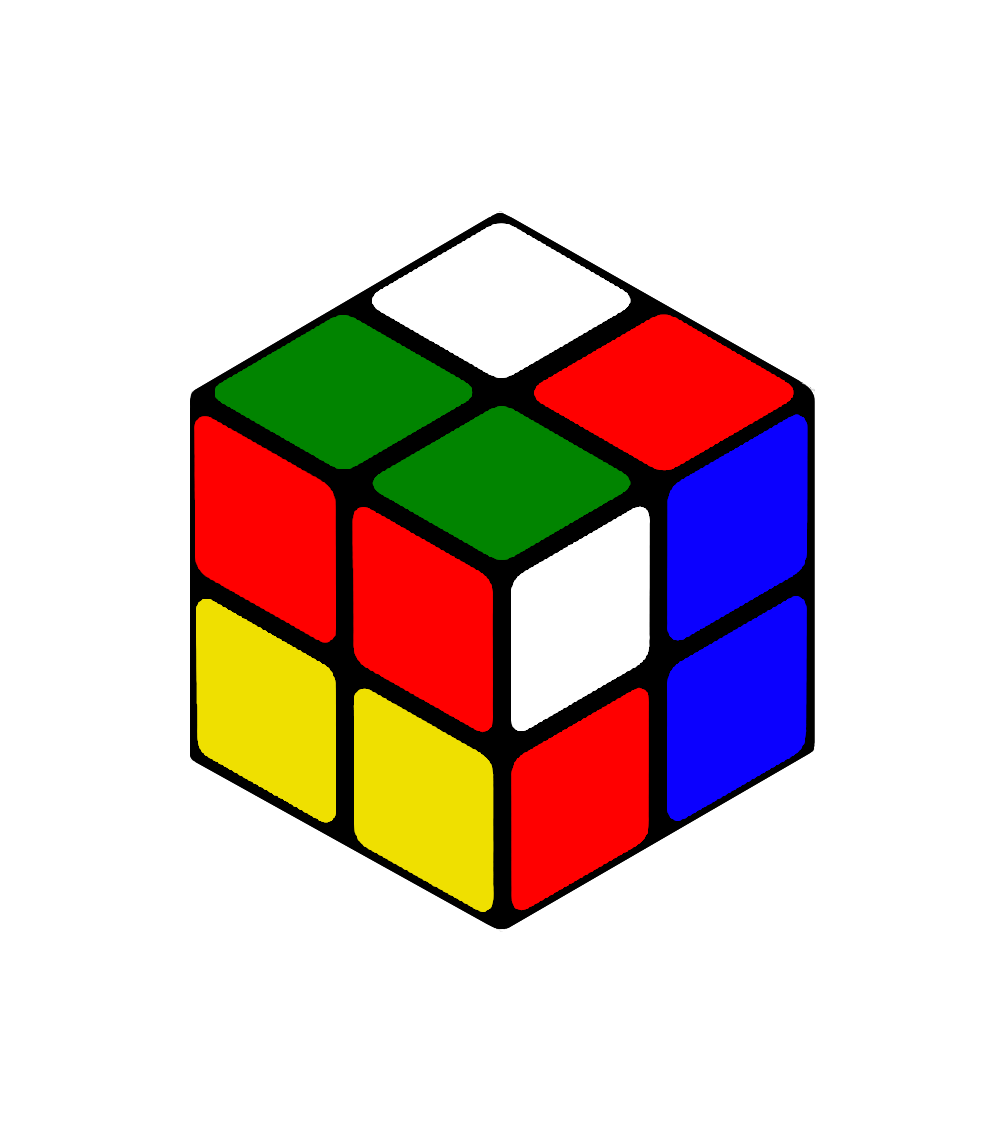
\includegraphics[scale=0.1]{RF.png}
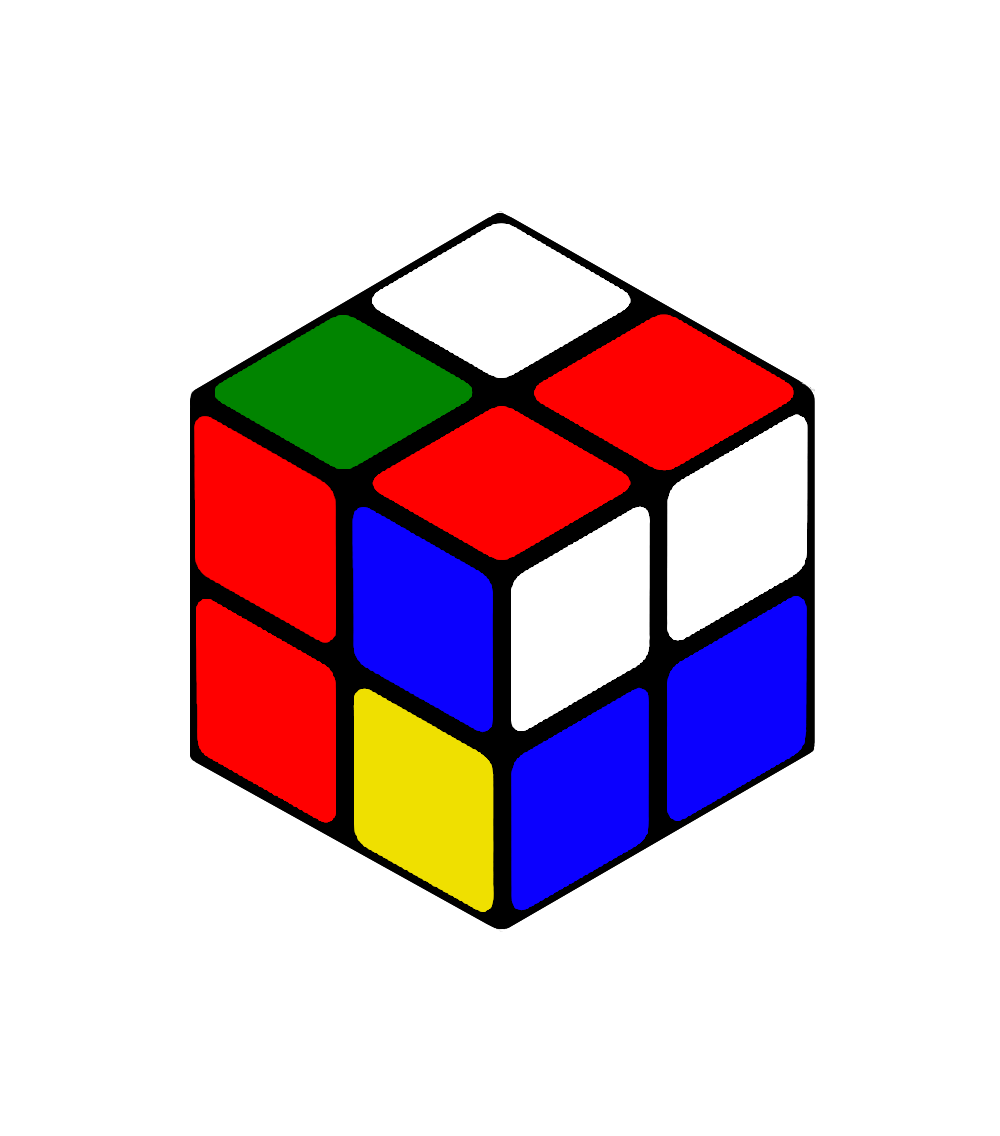
\includegraphics[scale=0.1]{FR.png}
\caption[Würfel nach Zügen $FR$ (links) und $RF$ (rechts)]{Würfel nach Zügen $FR$(links) und $RF$(rechts)}
\label{12}
\end{figure}
Außerdem wäre das Lösen des Würfels trivial, wenn die Kommutativität gelten würde.\cite{TD} Die Reihenfolge der gedrehten Ebenen wäre dann egal und man müsste nur die Anzahl beachten. 
Es gilt also nicht $\forall \  Z_1, Z_2 \in \Gtwo. Z_1 \circ Z_2 = Z_2 \circ Z_1$. Der $\circ$-Operator der Gruppe ist also nicht kommutativ. 

%
%
%
%
%
%
%
%
%
%
%=======================================================================================================
%
%
%
%
%
%
%
%
%
%
\subsection*{Züge als Gruppenoperation}\addcontentsline{toc}{subsection}{\protect\numberline{}Züge als Gruppenoperation}

Im Folgenden wird eine Gruppenoperation beschrieben, die eine Würfelkonfiguration durch das Ausführen eines Zuges auf eine neue Würfelkonfiguration abbildet. Bei Gruppenoperationen beeinflussen die Elemente einer Gruppe eine Menge. In diesem Fall beeinflussen die Züge des Würfels die Konfiguration des Würfels. Es handelt sich um eine Rechtsoperation, die im Kapitel \ref{11} beschrieben wurde.

Der Punktoperator ist definiert als $\cdot: M_C \times \Gtwo \rightarrow M_C$. Wenn der Zauberwürfel in einer Konfiguration $C=(\sigma, x)$ aus der Menge der Konfigurationen $M_C$ ist, wird er durch das Ausführen eines Zuges $Z \in \Gtwo$ in eine neue Konfiguration gebracht. Diese Konfiguration wird als $(C \cdot Z) \in M_C$ geschrieben.
Die folgenden beiden Eigenschaften müssen bei der Rechtsoperation gelten:

\begin{description}
\item [$\boldsymbol{C \cdot N = x}$ für alle $\boldsymbol{C \in M_C}$ und das neutrale Element $\boldsymbol{N \in \Gtwo}$] 
\ \\
Wenn der leeren Zug $N$ ausgeführt wird, wird die Konfiguration des Würfels nicht verändert. Es gilt also $C \cdot N = C$. 

\item [$\boldsymbol{C \cdot (Z_1 \circ Z_2) = (c \cdot Z_1) \cdot Z_2}$ für alle $\boldsymbol{Z_1, Z_2 \in \Gtwo}$ und $\boldsymbol{c \in M_C}$]
\ \\
Angenommen der Würfel befindet sich in der Konfiguration $C$. Wenn nun der Zug $Z_1 \in \Gtwo$ ausgeführt wird, ist die neue Konfiguration des Würfels $C \cdot Z_1$. Wenn nun noch ein weiterer Zug $Z_2 \in \Gtwo$ ausgeführt wird, ist die neue Konfiguration des Würfels $(C \cdot Z_1) \cdot Z_2$. 
Anders gesagt: Der Würfel hat in Konfiguration $C$ gestartet und der Zug $Z_1 Z_2$ wurde ausgeführt. Man kann die neue Konfiguration auch als $C \cdot (Z_1 Z_2)$ schreiben und somit gilt $(C \cdot Z_1) \cdot Z_2 = C \cdot (Z_1 Z_2)$. 
\end{description}

%
%
%
%
%
%
%
%=======================================================================================================
%
%
%
%
%
\subsection*{Rotation des Würfels}\addcontentsline{toc}{subsection}{\protect\numberline{}Rotation des Würfels}

Der \Ttwo Würfel hat im Gegensatz zum \Tthree Würfel keine Mittelsteine, die fest darüber entscheiden, welche Seite die obere Seite ist. 
Der \Ttwo Würfel kann also im gelösten Zustand sein, ohne dass die obere Seite weiß ist. Deshalb muss es möglich sein, den Würfel ganz zu rotieren, ohne einen Zug auszuführen.
Das soll im nächsten Abschnitt als Äquivalenrelationen umgesetzt werden. Dafür werden die Rotationsmöglichkeiten des Würfels in diesem Abschnitt definiert.
Um die Drehungen zu benennen, werden die Achsen des Würfels als $x, y$ und $z$ definiert. Das kann man in Abbildung \ref{15} sehen.
\begin{figure}[h]
\centering
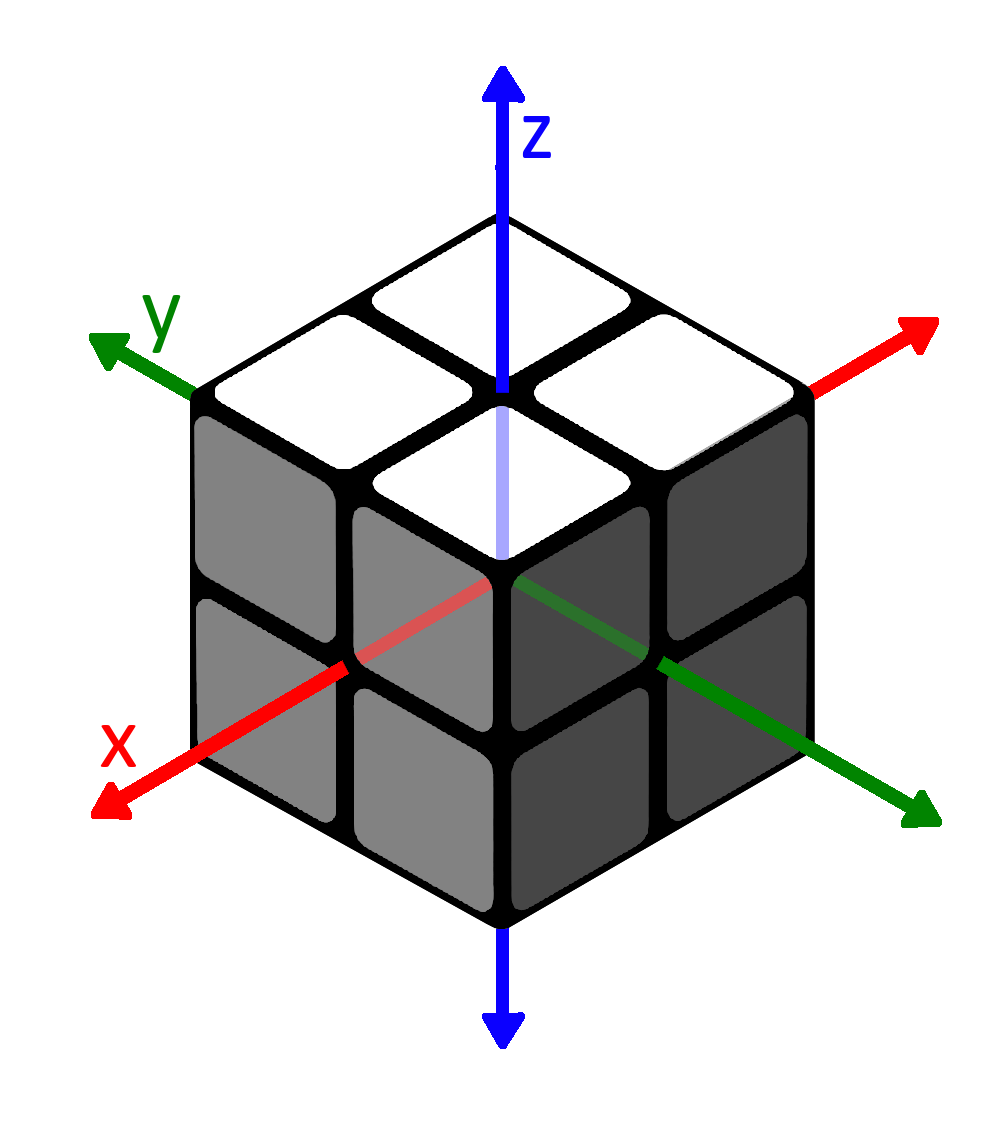
\includegraphics[scale=0.13]{Pfeile.png}
\caption[Würfel mit $x, y$ und $z$-Achsen]{Würfel mit $x, y$ und $z$-Achsen}
\label{15}
\end{figure} 

Nun kann man für die möglichen Rotationen des Würfels Nachfolgekonfigurationen festlegen. 
Dazu werden zuerst die einzelnen Rotationen des Würfels benannt. 

\begin{tabular}{cl}
\toprule
\textbf{Abkürzung} & \textbf{Beschreibung der Rotation} \\
\midrule
$Z_l$ & Rotation des Würfels um die $z$-Achse nach links (gegen den Uhrzeigersinn)\\

$Z_r$ & Rotation des Würfels um die $z$-Achse nach rechts (im Uhrzeigersinn)  \\

$Y_l$ & Rotation des Würfels um die $y$-Achse nach links (gegen den Uhrzeigersinn)\\

$Y_r$ & Rotation des Würfels um die $y$-Achse nach rechts (im Uhrzeigersinn)  \\

$X_l$ & Rotation des Würfels um die $x$-Achse nach links (gegen den Uhrzeigersinn)\\

$X_r$ & Rotation des Würfels um die $x$-Achse nach rechts (im Uhrzeigersinn) \\
\bottomrule
\end{tabular} 


Die Rotationen sind nicht minimal definiert, da beispielsweise $Z_l$ das gleiche wie ${Z_r}^3$ ist. Dies dient der Anschaulichkeit. 

Die Steine werden durch eine Rotation alle an einen neuen Platz gebracht. Anders als bei der Drehung der Ebenen, wo nur einige Steine die Position ändern, ändern hier alle Steine die Position, ohne dass der Würfel verändert wird, da er komplett gedreht wird. 

Anhand der Rotation $Z_r$, also einer Rotation des kompletten Würfels um die $z$-Achse um $90^\circ$ im Uhrzeigersinn, wird nun die Veränderung der Würfelpositionen gezeigt. Die Rotation $Z_r$ sieht man in Abbildung \ref{16}.
\begin{figure}[h]
\centering
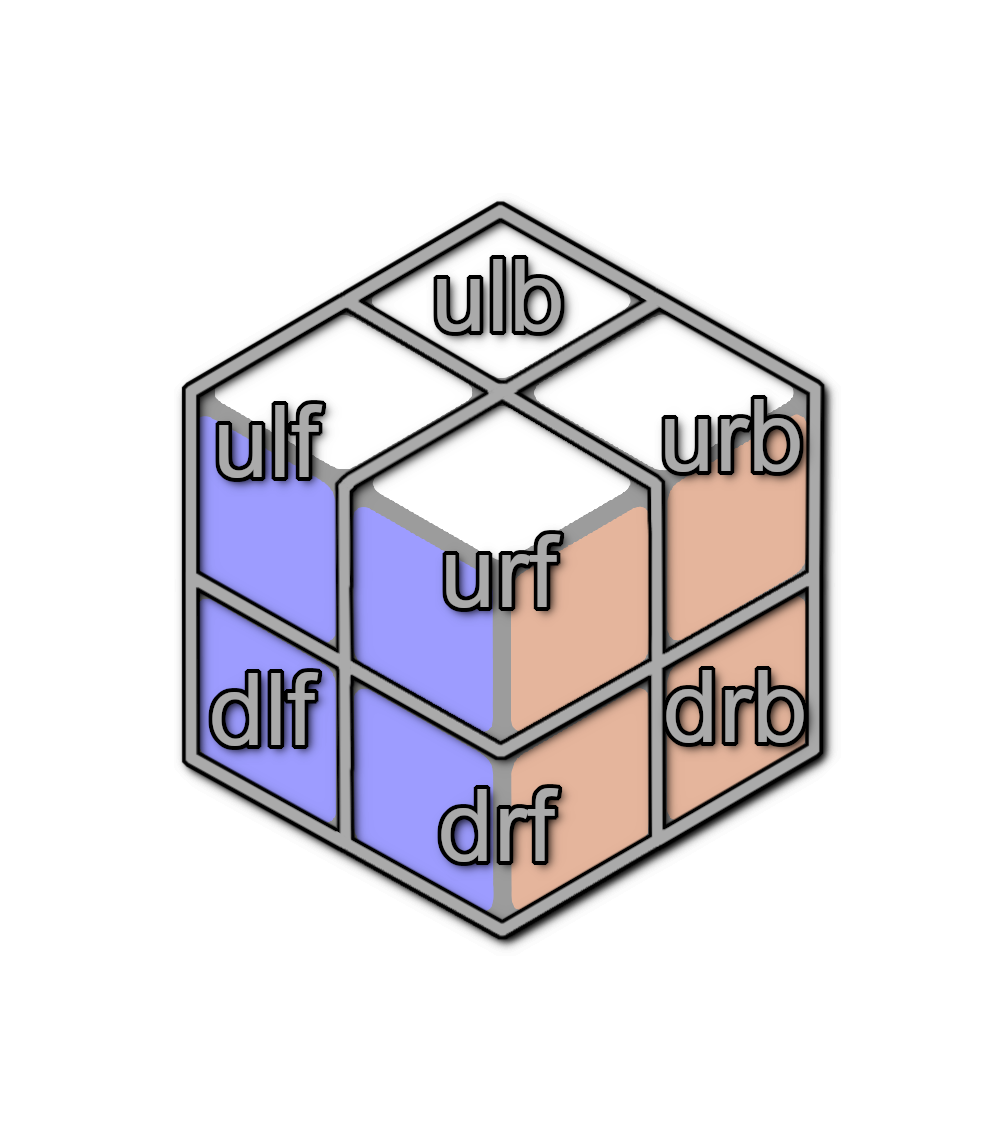
\includegraphics[scale=0.13]{auf_ulf.png}
\caption{Würfel nach Rotation um $z$-Achse}
\label{16}
\end{figure}
Da bei den Rotationen alle Steine die Position wechseln, muss es 8 Funktionen $\delta$ geben, also für jeden Eckstein eine Funktion $\delta$:
\begin{align*}
\delta_{Z_r}(urf) = ulf \ \ \ \ \ \ \delta_{Z_r}(ulf) = ulb \ \ \ \ \ \ \delta_{Z_r}(ulb) = urb \ \ \ \ \ \ \delta_{Z_r}(urb) = urf \\
\delta_{Z_r}(drf) = dlf \ \ \ \ \ \ \delta_{Z_r}(dlf) = dlb \ \ \ \ \ \ \ \delta_{Z_r}(dlb) = drb \ \ \ \ \ \ \delta_{Z_r}(drb) = drf
\end{align*}

Wenn man das nun in der Form $i \mapsto j$ schreibt, erhält man: 
\begin{align*}
urf \mapsto ulf \ \ \ \ \ \ \ \ ulf \mapsto ulb \ \ \ \ \ \ \ \ ulb \mapsto urb \ \ \ \ \ \ \ \ urb \mapsto urf \\
drf \mapsto dlf \ \ \ \ \ \ \ \ dlf \mapsto dlb \ \ \ \ \ \ \ \ \ dlb \mapsto drb \ \ \ \ \ \ \ \ drb \mapsto drf
\end{align*}

In der Zykel-Schreibweise sieht die Veränderung der Steinnamen dann so aus: \\
$\delta_{Z_r}=(urf \ ulf \ ulb \ urb)(drf \ dlf \ dlb \ drb )$ 

Alle Rotationen sehen in Zykel-Schreibweise folgendermaßen aus:
\begin{align*}
\delta_{Z_r} & = (ulf \ ulb \ urb \ urb) \ (dlf \ dlb \ drb \ drf)\\
\delta_{Z_l} & = (ulf \ urf \ urb \ ulb) \ (dlf \ drf \ drb \ dlb)\\
\delta_{Y_r} & = (ulf \ ulb \ dlb \ dlf) \ (urf \ urb \ drb \ drf)\\
\delta_{Y_l} & = (ulf \ dlf \ dlb \ ulb) \ (urf \ drf \ drb \ urb)\\
\delta_{X_r} & = (ulf \ urf \ drf \ dlf) \ (urb \ ulb \ dlb \ drb)\\
\delta_{X_l} & = (ulf \ dlf \ drf \ urf) \ (urb \ ulb \ dlb \ drb)
\end{align*}
Bei den Rotationen wird (analog zu den Zügen) die mehrfache Ausführung einer Roatation mit der Exponentenschreibweise geschrieben. 
Somit gilt dann auch hier $RRRR=R^4=N$ (für $R \in \{{Z_r}, {Z_l}, {Y_r}, {Y_l}, {X_r}, {X_l} \}$) und $R^0=N$ (für alle Rotationen). ($N$ ist das neutrale Element, also der leere Zug und $R$ eine beliebige Rotation des Würfels.) 
Analog zu den Zügen gilt bei den Rotationen also für jede Rotation: 
\begin{align*}
\forall R \in \{{Z_r}, {Z_l}, {Y_r}, {Y_l}, {X_r}, {X_l} \}, n \in \mathbb{N} \ . \ R^n=R^{n \mod 4}
\end{align*}

%
%
%
%
%
%
%
%
%
%
%=======================================================================================================
%
%
%
%
%
%
%
%
%
%
%\hspace*{2cm}

%\color{gray}


%\subsection*{Äquivalenzrelationen der Rotationen (Fehlversuch)}\addcontentsline{toc}{subsection}{\protect\numberline{}Äquivalenzrelationen der Rotationen (Fehlversuch)}


%Um die Rotationen des Würfels umzusetzen, führe ich Äquivalenzrelationen ein. \\
%Eine Relation $R \subseteq A \times A$ heißt Äquivalenzrelation auf $A$, wenn für alle $x, y, z \in A$ die drei folgenden Eigenschaften gelten: Reflexivität, Symmetrie, Transitivität. \cite{Buch} \\
%\\
%In dem Fall der Gruppe $(\Gtwo, \circ)$ handelt es sich um eine Relation von zwei Zügen $Z_1, Z_2 \in \Gtwo$. \\ 
%Ich führe für jede Rotationsrichtung eine Relation ein. Es gibt dann also $\sim_{Z_r}, \sim_{Z_l}, \sim_{Y_r}, \sim_{Y_l}, \sim_{X_r}, \sim_{X_l}$. \\ 


%\begin{tabular}{l l}

%$Z_1 \sim_{Z_r} Z_2$ & $:\Leftrightarrow \ \ \ \ \  Z_1$ und $Z_rZ_2$  ergeben die gleiche Würfelkonfiguration\\

%\end{tabular}
%\\
%$Z_rZ_2$ steht für den Zug $Z_2$, der nach einer Rechtsrotation des Würfels ausgeführt wird. \\
%\\
%Die anderen Rotationsrelationen definiere ich wie folgt: 

%\begin{tabular}{l l l}

%$Z_1 \sim_{Z_l} Z_2$ & $:\Leftrightarrow \ \ \ \ \  Z_1$ und $Z_lZ_2$ & ergeben die gleiche Würfelkonfiguration \\
%$Z_1 \sim_{Y_r} Z_2$ & $:\Leftrightarrow \ \ \ \ \  Z_1$ und $Y_rZ_2$ & ergeben die gleiche Würfelkonfiguration\\
%$Z_1 \sim_{Y_l} Z_2$ & $:\Leftrightarrow \ \ \ \ \  Z_1$ und $Y_lZ_2$ & ergeben die gleiche Würfelkonfiguration\\
%$Z_1 \sim_{X_r} Z_2$ & $:\Leftrightarrow \ \ \ \ \  Z_1$ und $X_rZ_2$ & ergeben die gleiche Würfelkonfiguration\\
%$Z_1 \sim_{X_l} Z_2$ & $:\Leftrightarrow \ \ \ \ \  Z_1$ und $X_lZ_2$ & ergeben die gleiche Würfelkonfiguration\\

%\end{tabular}
%\\
%\\
%\\
%\\
%Damit $\sim_{Z_r}, \sim_{Z_l}, \sim_{Y_r}, \sim_{Y_l}, \sim_{X_r}$ und $\sim_{X_l}$ Äquivalenzrelationen sind, müssen Reflexivität, Symmetrie und Transitivität gelten, was ich im folgenden Abschnitt beweise. Ich nutze das Symbol $\sim$ für alle Elemente aus  $\{ \sim_{Z_r}, \sim_{Z_l}, \sim_{Y_r}, \sim_{Y_l}, \sim_{X_r}, \sim_{X_l}\}$ und $W$ als beliebige Würfelrotation (${Z_r}, {Z_l}, {Y_r}, {Y_l}, {X_r}$ oder ${X_l}$).\\



%\begin{itemize}

%\item Reflexivität: \\
%Für die Reflexivität muss $x \sim x$ gelten. \\
%Da alle $\sim \in \{ \sim_{Z_r}, \sim_{Z_l}, \sim_{Y_r}, \sim_{Y_l}, \sim_{X_r}, \sim_{X_l}\}$ durch die Gleichheit definiert sind, gilt:
%\begin{align*}
%Z_1 \sim_W Z_2 : & \Leftrightarrow \ \ \  Z_1 \ und  \ WZ_2 \ ergeben \ die \ gleiche \ W"urfelkonfiguration\\
%& \Leftrightarrow \ \ \ C \cdot Z_1=C \cdot WZ_2 \\
%& \Leftrightarrow \ \ \ Z_1=WZ_2
%\end{align*}
%$\lightning$ Das gilt aber leider nicht, wenn $Z_1=Z_2$ gilt. Denn identische Züge ergeben nicht das gleiche, wenn der Würfel vor einem Zug rotiert wird und vor dem anderen nicht. \\
%\\


%\item Symmetrie $\lightning$%:  \\
%Für die Symmetrie muss gelten: Aus $x \sim y \ folgt \ y \sim x$. \\
%Auch das gilt, da alle $\sim \in \{ \sim_{Z_r}, \sim_{Z_l}, \sim_{Y_r}, \sim_{Y_l}, \sim_{X_r}, \sim_{X_l}\}$ durch die Gleichheit definiert sind.  

%\item Transitivität $\lightning$

%\end{itemize}

%Diese Ansatz dieser Äquivalenzrelationen funktioniert so nicht, da die Reflexivität, Symmetrie und Transitivität nicht erfüllt sind. \\ 

%falsch

%
%
%
%
%
%
%
%
%
%
%=======================================================================================================
%
%
%
%
%
%
%
%
%
%
\color{black}

\subsection*{Äquivalenzrelationen der Rotationen}\addcontentsline{toc}{subsection}{\protect\numberline{}Äquivalenzrelationen der Rotationen}

Da der \Ttwo Würfel im Gegensatz zum \Tthree Würfel keine feste Ausrichtung hat, werden in diesem Abschnitt Äquivalenzrelationen eingeführt, um die Rotationen des Würfels umzusetzen.
Für Äquivalenzrotaionen müssen die drei folgenden Eigenschaften gelten: Reflexivität, Symmetrie, Transitivität. In Kapitel \ref{11} findet sich die Definition und Erklärung.

In dem Fall der Gruppe $(\Gtwo, \circ)$ handelt es sich um eine Relation von zwei Zügen $Z_1, Z_2 \in \Gtwo$. 

Die Äquivalenzrelation der Rotation wird hier so definiert: 


\begin{tabular}{l l}
$Z_1 \sim Z_2 := \ $  & $Z_1$ \textit{und} $Z_2$ \textit{ergeben (mit optionaler Rotation) die gleiche }\\
\  & \textit{Würfelkonfiguration} \\
\end{tabular} 
\\

Daraus ergibt sich $Z_1 \sim Z_2 :\Leftrightarrow \ Z_1 = WZ_2$ mit $W$ als Element (oder Kombination von Elementen) aus $\{{Z_r}, {Z_l}, {Y_r}, {Y_l}, {X_r}, {X_l}, N\}$, wobei $N$ die \textit{leere} Rotation darstellt, also keine Rotation des Würfels. 
Somit ergibt sich beispielsweise $F \sim L \Leftrightarrow F = Z_rL$, da eine Drehung der vorderen Ebene und eine Drehung des Würfels nach links mit einer Drehung der linken Ebene die gleiche Würfelkonfiguration ergeben. Der Würfel ist dann nur verschieden ausgerichtet. 
In Abbildung \ref{1} sieht man dieses Beispiel nochmal grafisch: Links befindet sich der gelöste Würfel, in der Mitte der gelöste Würfel nach dem Zug $F$ und rechts der gelöste Würfel nach dem Zug $Z_rL$. Die beiden rechten Würfel sind in der gleichen Konfigurationen, aber anders gedreht.
\begin{figure}[h]
\centering
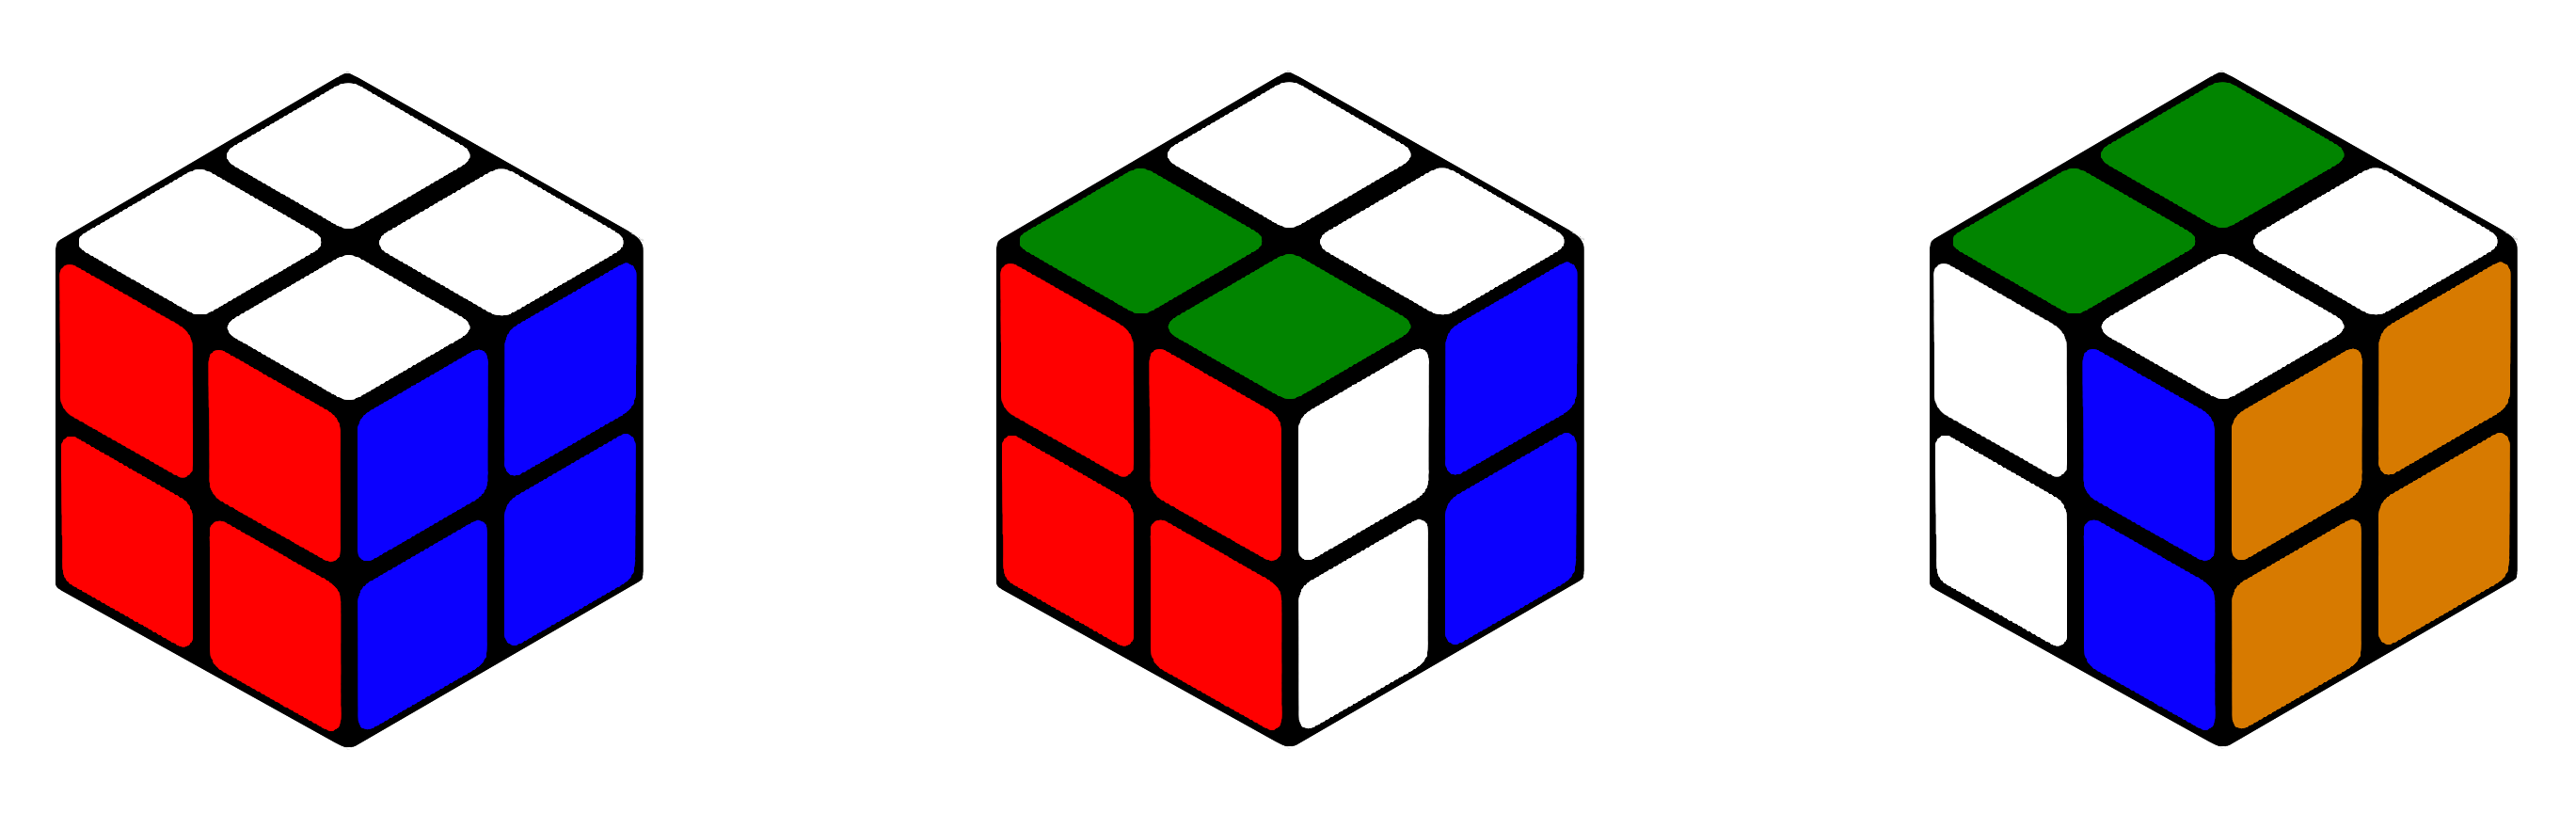
\includegraphics[scale=0.15]{3_wuerfel.png}
\caption[Würfel gelöst, nach Zug $F$ und nach $Z_rL$]{Würfel gelöst (links), nach Zug $F$ (mitte) und nach $Z_rL$(rechts)}
\label{1}
\end{figure}

Damit $\sim$ eine Äquivalenzrelation ist, müssen Reflexivität, Symmetrie und Transitivität gelten, was im folgenden Abschnitt bewiesen wird.

\begin{description}


\item [Reflexivität] \ \\
Für die Reflexivität muss $Z \sim Z$ für alle $Z \in \Gtwo$ gelten. 
\begin{align*}
Z_1 \sim Z_2 : & \Leftrightarrow  Z_1 = WZ_2
\end{align*}
Es wird $W$ als $N$ gewählt, so dass keine Rotation ausgeführt wird.
\begin{align*}
Z_1 \sim Z_2 : & \Leftrightarrow  Z_1 = WZ_2 \\
\ & \Leftrightarrow Z_1=N Z_2 \\
\ & \Leftrightarrow Z_1 = Z_2
\end{align*}
Also gilt die Reflexivität für $\sim$, da für $Z_1 \sim Z_2$ mit $W=N$ immer $Z_1 = Z_2$ gilt.

\item [Symmetrie] \ \\
Für die Symmetrie muss gelten: Aus $Z_1 \sim Z_2$ folgt $Z_2 \sim Z_1$.
\begin{align*}
Z_1 \sim Z_2 & \Rightarrow Z_2 \sim Z_1 \\
mit \ Z_1 \sim Z_2 : & \Leftrightarrow  Z_1 = WZ_2 \\
\Leftrightarrow Z_1 = W_1 Z_2 & \Rightarrow Z_2 = W_2 Z_1
\end{align*}
Das gilt, wenn $W_2$ das Inverse von $W_1$ ist. Das Inverse ist die Rotation um die gleiche Achse, aber in die andere Richtung. 
Das Inverse von $W$ wird als $W^{-1}$ geschrieben.
Das sind die Rotationen mit den dazugehörigen Inversen:

\begin{center}
\begin{tabular}{lccccccc}
Rotation $W$ & ${Z_r}$ & ${Z_l}$ &  ${Y_r}$ & ${Y_l}$ & ${X_r}$ & ${X_l}$ & $N$ \\
\hline
Inverses \hspace*{0.1em} $W^{-1}$ & ${Z_l}$ & ${Z_r}$ &  ${Y_l}$ & ${Y_r}$ & ${X_l}$ & ${X_r}$ & $N$ \\
\end{tabular} 
\end{center}
Dann gilt: 
\begin{align*}
Z_1 = W Z_2 & \Rightarrow Z_2 = W^{-1} Z_1
\end{align*}
Das gilt, da durch $W^{-1}$ der Würfel in die entgegengesetzte Richtung rotiert wird und die Züge somit wieder die gleiche Würfelkonfiguration ergeben.
Also gilt die Symmetrie für $\sim$.


\item [Transitivität] \ \\
Es muss gelten: Aus $Z_1 \sim Z_2$ und $Z_2 \sim Z_3$ folgt $Z_1 \sim Z_3$.
\begin{alignat*}{3}
& Z_1 \sim Z_2 && \wedge Z_2 \sim Z_3 && \Rightarrow Z_1 \sim Z_3 \\
\Leftrightarrow \ & Z_1 = W_1Z_2 \ && \wedge Z_2 = W_2Z_3 \ && \Rightarrow Z_1 = W_3Z_3
\end{alignat*}
Das gilt für $W_3=W_1W2$.
\begin{alignat*}{3}
\Leftrightarrow \ & Z_1 = W_1Z_2 \ && \wedge Z_2 = W_2Z_3 \ && \Rightarrow Z_1 = W_1W_2Z_3 
\end{alignat*}
Da die Züge $Z_1$ und $Z_2$ mit der Rotation $W_1$ die gleiche Würfelkonfiguration ergeben, und die Züge $Z_2$ und $Z_3$ nach der Rotation $W_2$ auch die gleiche Würfelkonfiguration ergeben, gilt das auch für die beiden Züge $Z_1$ und $Z_3$ nach der Rotation $W_3=W_1W_2$, da dann alle nötigen Rotationen durchgeführt wurden.

\end{description}
%
%
%
%
%
%
%
%
%
%
%=======================================================================================================
%
%
%
%
%
%
%
%
%
%
\subsection*{Ordnung der Züge}\addcontentsline{toc}{subsection}{\protect\numberline{}Ordnung der Züge}
Wie bereits beschrieben, gilt $\forall Z \in \{ U, D, F, B, L, R \}, n \in \mathbb{N} \ . \ Z^n=Z^{n \mod 4}$, da alle Steine des Würfels in ihrer vorherigen Position bleiben, wenn eine Ebenen- oder eine Würfelrotation vier mal hintereinander ausgeführt wird. Deshalb werden die Züge $U, D, F, B, L, R$ als Züge der Ordnung 4 bezeichnet. 
Die Exponentenschreibweise kann man für alle Züge aus $\Gtwo$ anwenden, auch wenn sie mehr als eine Ebene rotieren, beispielsweise bei $LLFF$. $(LLFF)^2$ entspricht dann $LLFFLLFF$ und $(LLFF)^3$ ist $LLFFLLFFLLFF$, was wieder die Ausgangsposition ergibt. 

Nicht nur die Züge $U, D, F, B, L, R$ kommen nach dem Wiederholen in den Ausgangszustand. Auch alle anderen Züge bringen den Würfel wieder in die Ausgangsposition des Zuges \cite{TD}. Es sind aber je nach Zug verschieden viele Wiederholungen nötig. Der Zug $(LLFF)$ hat beispielsweise die Ordnung 3, da der Würfel sich nach dreifacher Wiederholung von $(LLFF)$ wieder in der Ausgangsposition befindet. Es gilt dann $(LLFF)^3 = N$.
Weitere Beispielzüge mit Angabe der Ordnung sind: ${R^4= N}$ (Ordnung 4), ${(RRFF)^3 = N}$ (Ordnung 3) oder auch ${(LF)^{15}=N}$ (Ordnung 15). 
Die genannten Beispiele kann man an einem \Ttwo Würfel einfach ausprobieren.
Dabei muss beachtet werden, dass die Ordnung die Anzahl der Durchführungen beschreibt, die benötigt wird, damit alle Steine wieder an der Ausgangsposition sind. Die Ausrichtung der Steine wird hier aber nicht berücksichtigt. 


Im folgenden Abschnitt wird bewiesen, dass die Würfelsteine wieder in die Ausgangspositionen gelangen, wenn man einen beliebigen Zug $Z \in \Gtwo$ wiederholt auf den Würfel anwendet.
Der folgende Beweis orientiert sich an dem Beweis aus dem Paper \textit{Group Theory via Rubik's Cube} von Tom Davis \cite{TD}: \\
Jedes Mal wenn ein Zug wiederholt wird, werden die Steine im Würfel neu angeordnet. \\ 
Da es eine endliche Anzahl an Würfelkonfigurationen gibt, muss eine Würfelposition wiederholt werden, wenn man den Zug oft genug durchführt. \\
Die Zahl der validen Würfelkonfigurationen ist zwar sehr groß, aber endlich. Also muss eine Position wiederholt werden, wenn man den Zug öfter ausführt, als es mögliche Würfelpositionen gibt. \\
Bei einem beliebigen Zug $Z \in \Gtwo$ gelangt man also irgendwann in eine Würfelposition, die sich wiederholt. Die wiederholende Würfelposition tritt zuerst nach $n \in \mathbb{N}$ Wiederholungen auf und das zweite Mal nach $m \in \mathbb{N}$ Wiederholungen. Das sieht dann so aus: $Z^n=Z^m$ mit $0 < n < m$. \\
Also gilt mit der Würfelkonfiguration $Z^{n-1} \neq Z^{m-1}$, da $m$ das zweite Vorkommen der gleichen Position repräsentiert. \\
Wenn $n=0$ ist, hat man $Z^0=N$, was den leeren Zug (bzw. das neutrale Element) repräsentiert. Der Würfel wird dabei nicht verändert und somit wird die Würfelposition bei jedem Zug $Z \in \Gtwo$ mit $Z^0$ wiederholt. \\
Es gilt $Z^n = Z^m$. Wenn man nun auf die gleiche Ausgangsposition $n$-mal oder $m$-mal $Z$ anwendet, kommt man in der gleichen Endposition an. \\
Wenn man nun $Z^{-1}$ anwendet, kommt man wieder in die gleiche Endposition. Dabei ist es egal, ob man vorher $n$-mal oder $m$-mal $Z$ ausgeführt hat, da man von der gleichen Startposition ausgehend in die gleiche Endposition kommt, wenn man den gleichen Zug ausführt. \\
Beim Anwenden von $Z^{-1}$ wird die letzte Ausführung von $Z$ wieder rückgängig gemacht. Wenn man $Z$ also $n$-mal ausführt und dann $Z^{-1}$ ausführt, ist es das gleiche wie $n-1$-mal $Z$ ausführen, also $Z^nZ^{-1}=Z^{n-1}$. Das gilt natürlich auch für $m$, also $Z^mZ^{-1}=Z^{m-1}$.\\
Demnach gilt dann $Z^{n-1}=Z^{m-1}$. Das widerspricht dann aber der Annahme, dass $m$ der kleinste Wert für eine Wiederholung der Position ist. Also muss $n=0$ sein, damit $m$ die erste Wiederholung einer Position repräsentiert. 

Daraus folgt: Wenn man den Zug wiederholt auf einen Würfel anwendet, kommen die Steine wieder in die Ausgangsposition.
 
%
%
%
%
%
%
%
%
%
%
%=======================================================================================================
%
%
%
%
%
%
%
%
%
%


\subsection*{Zykelstruktur}\addcontentsline{toc}{subsection}{\protect\numberline{}Zykelstruktur}


Anhand der Zykelstruktur lässt sich die Ordnung des jeweiligen Zuges bestimmen. Die Ordnung beschreibt die Anzahl der Wiederholungen, die ein Zug durchgeführt werden muss, damit die Steine die gleiche Anordnung wie zu Beginn des Zuges haben. Dabei geht es um die Steinpositionen und nicht um die Steinausrichtungen.
Der Würfel kann also alle Steine an der richtigen Position haben und trotzdem ungelöst sein, da die Steine verdreht sein können. 

Der Zug $U$ als $\sigma_U =\ (ulf \ ulb \ urb \ urf) $ (eine Drehung der oberen Ebene um $90^\circ$ im Uhrzeigersinn) besteht aus einem 4-elementigen Zykel.
Wenn der Zug $U$ also viermal ausgeführt wird, befindet sich der Würfel wieder in seiner vorherigen Position: 
\begin{center}
\centering
\begin{tabular}{ccccc}
\toprule
\textbf{Ausführung} & \textbf{ulf} & \textbf{ulb} & \textbf{urb} & \textbf{urf} \\
\midrule
1 & ulb & urb & urf & ulf \\

2 & urb & urf & ulf & ulb \\

3 & urf & ulf & ulb & urb \\

4 & ulf & ulb & urb & urf \\
\bottomrule
\end{tabular}
\end{center}

Die vierte Zeile der Tabelle hat die selbe Anordnung der Steine wie die oberste Zeile (vor Ausführung von $U$). 
Somit hat die beschriebene Ebenenrotation $U$ die Ordnung 4. Das gilt auch für jede andere Ebenenrotation ($D, F, B, L, R$).
Es gilt also für jeden Zug $Z$, der aus nur einem $n$-elementigen Zykel besteht: \\ 
${\forall \ Z \in \Gtwo\ mit \ \sigma_Z=(i_1 \ i_2 \ ... \ i_n), n \in \mathbb{N} \ . \  Z^n=N }$. 
Wenn man $Z$ mehrfach ausführt, kommt man nach jeder $n$-ten Wiederholung in den Ausgangszustand. \cite{TD} 
Es gilt also auch 
${\forall \ Z \in \Gtwo\ mit \ Z=(i_1 \ i_2 \ ... \ i_n), n,k \in \mathbb{N} \ . \  Z^{k*n}=1 }$.
Auch bei komplexeren Zügen kann anhand der Zykelstruktur die Ordnung bestimmt werden. Dazu muss das kleinste gemeinsame Vielfache aller Zykelgrößen bestimmt werden. \cite{TD}

 
Der besseren Übersichtlichkeit halber, sind die Zykel aller Züge in Abbildung \ref{2} grafisch dargestellt.
Dieser Graph vereinfach das Ablesen der Zykel, wenn bei einem Zug mehrere Ebenenrotationen kombiniert werden.
\begin{figure}[H]
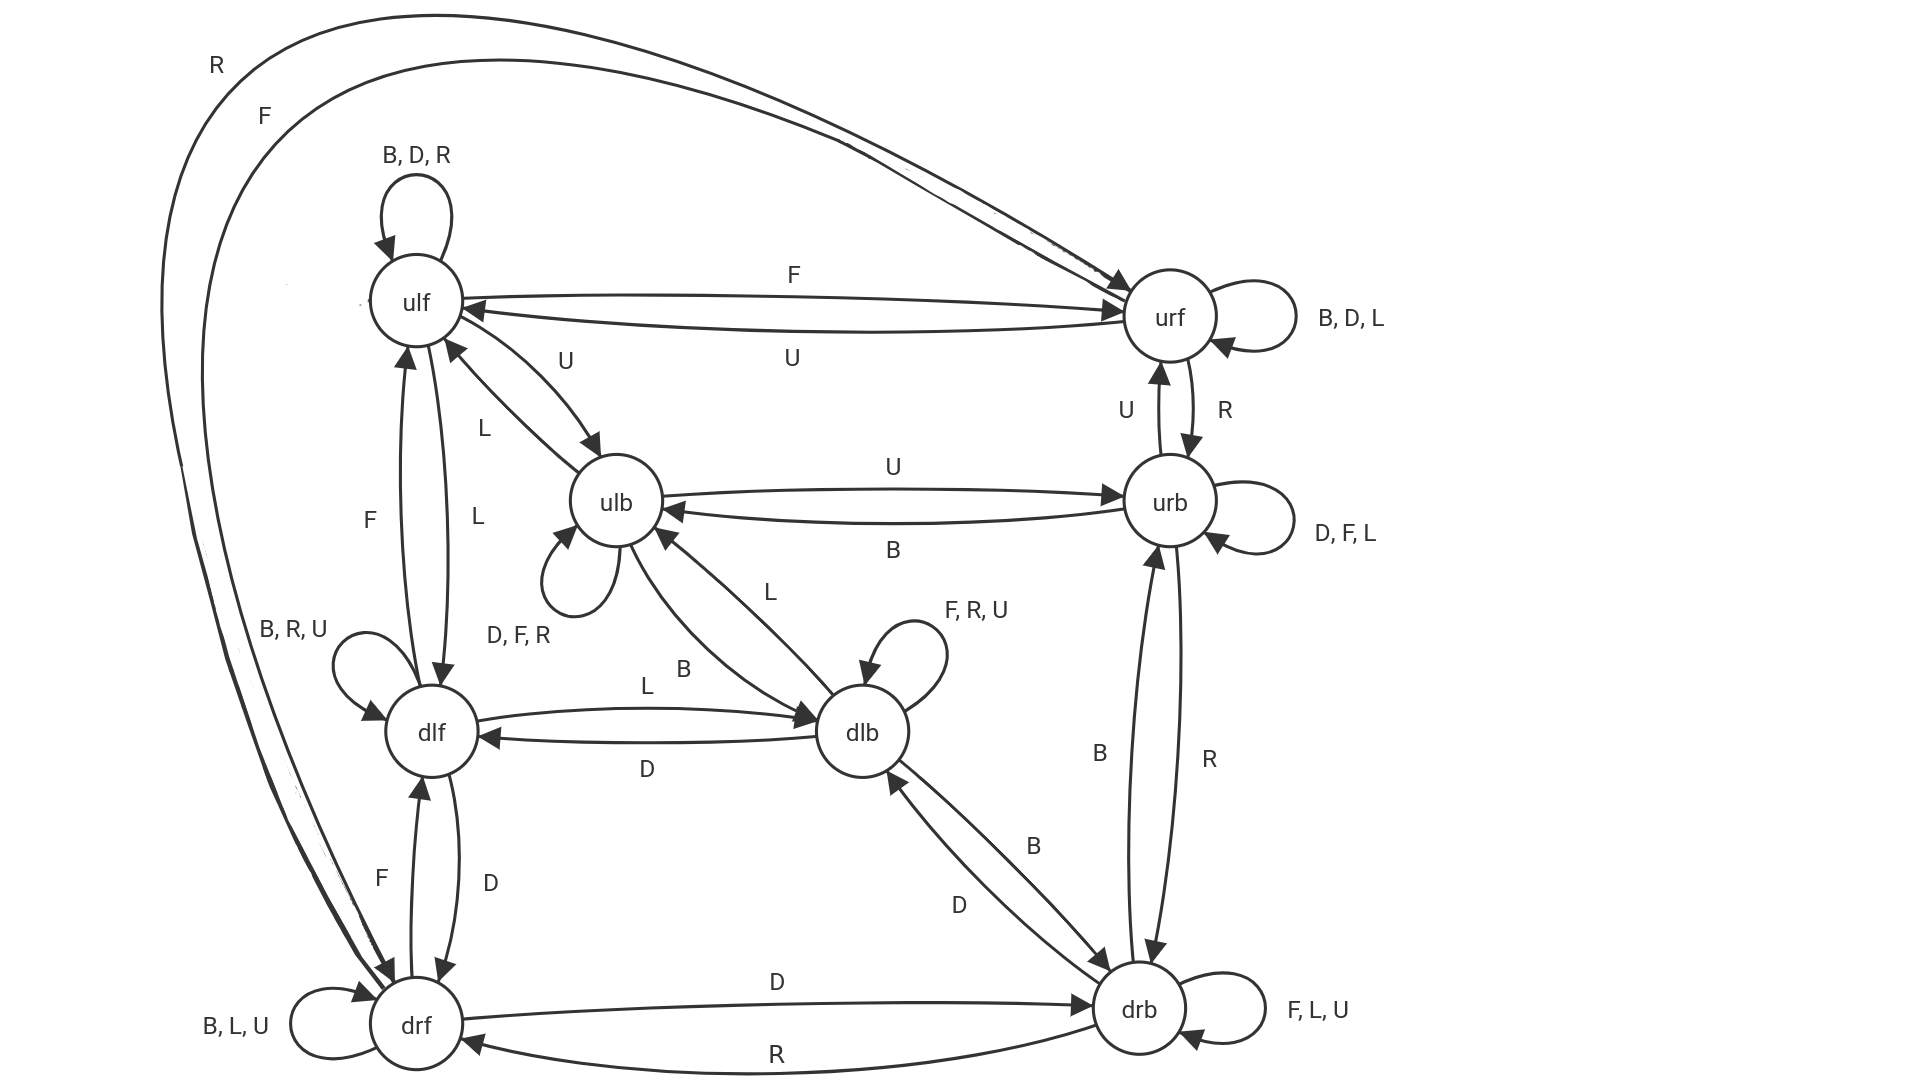
\includegraphics[scale=0.3]{graph_zug.png}
\caption[Graph aller Zugpermutationen]{Graph aller Zugpermutationen}
\label{2}
\end{figure}

So kann man nun anhand des Beispielzuges $LLFF$ die Zykelstruktur darstellen. 
Zuerst wird eine Tabelle erstellt, die jede Position auf ihre neue Position abbildet. Der Zug $LLFF$ setzt sich aus den Zügen $L$ und $F$ zusammen. 

\begin{center}
\begin{tabular}{ccccccccc}
\toprule
\textbf{Zug} & \textbf{ulb} & \textbf{urb} & \textbf{ulf} & \textbf{urf} & \textbf{dlb} & \textbf{drb} & \textbf{dlf} & \textbf{drf} \\
\midrule

L & ulf & \textcolor{gray}{urb} & dlf & \textcolor{gray}{urf} & ulb & \textcolor{gray}{drb} & dlb & \textcolor{gray}{drf} \\

L & dlf & \textcolor{gray}{urb} & dlb & \textcolor{gray}{urf} & ulf & \textcolor{gray}{drb} & ulb & \textcolor{gray}{drf} \\

F & ulf & \textcolor{gray}{urb} & \textcolor{gray}{dlb} & drf & urf & \textcolor{gray}{drb} & \textcolor{gray}{ulb} & dlf \\

F & urf & \textcolor{gray}{urb} & \textcolor{gray}{dlb} & dlf & drf & \textcolor{gray}{drb} & \textcolor{gray}{ulb} & ulf \\
\bottomrule
\end{tabular}
\end{center}

Die grauen Positionen bleiben bei der jeweiligen Ebenenrotation unverändert. 
Grafisch dargestellt sieht man die Zykel des Zuges $LLFF$ in Abbildung \ref{17}. 
\begin{figure}[h]
\centering
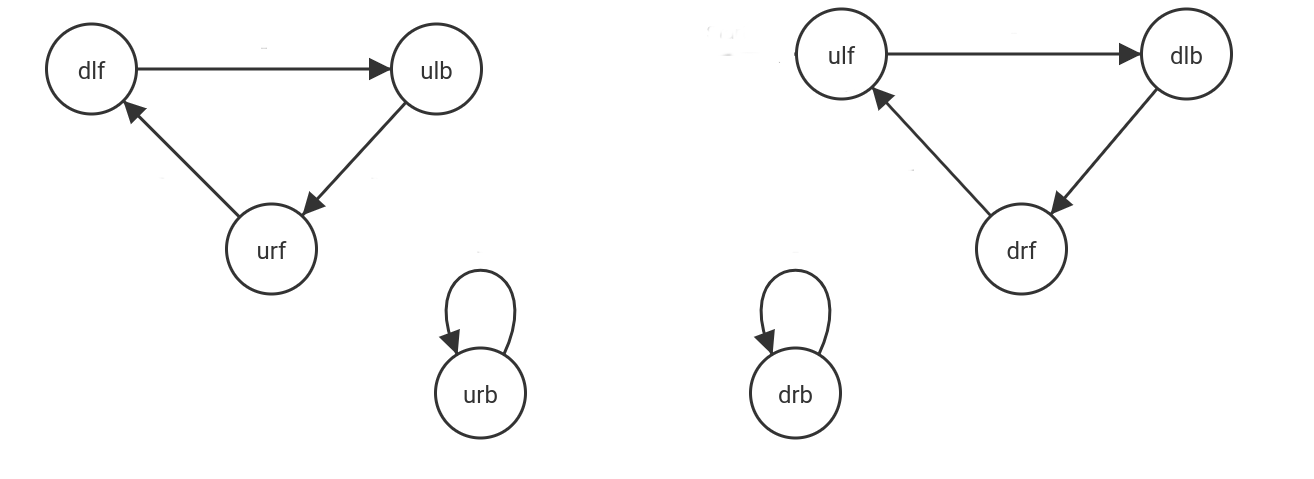
\includegraphics[scale=0.25]{zykel_LLFF.png}
\caption[Zykel des Zuges $LLFF$]{Zykel des Zuges $LLFF$}
\label{17}
\end{figure}
In Zykelschreibeweise also $\sigma_{LLFF}=(dlf \ ulb \ urf)(ulf \ dlb \ drf)$.
Da es also zwei Zykel der Länge drei gibt, befinden sich alle Würfelsteine nach drei Zügen ($KGV(3,3,1,1)=3$) wieder in ihrer Ausgangsposition. 
In diesem Fall sind die Steine nicht nur an der richtigen Position sondern auch so ausgerichtet, wie zu Beginn des Zuges. 
Außerdem kann man erkennen, dass sechs der acht Steine bei dem Zug $LLFF$ bewegt werden. Die anderen beiden ($urb$ und $drb$) bleiben unverändert. 

%
%
%
%
%
%
%
%
%
%
%=======================================================================================================
%
%
%
%
%
%
%
%
%
%
\subsection*{Äquivalenz von Zügen}\addcontentsline{toc}{subsection}{\protect\numberline{}Äquivalenz von Zügen}


Es kann schwierig sein, die Äquivalenz von Zügen oder Roatationen anhand der Funktionen ($\sigma$ und $\delta$) in der Zykelschreibweise zu erkennen. 
Das liegt daran, dass man die Zykel in verschiedener Reihenfolge schreiben kann. So ist der Zug $U$ beispielsweise $ (ulf \ ulb \ urb \ urf)$, aber auch $(urb \ urf \ ulf \ ulb)$.
Um das zu vereinfachen, werden die Würfelpositionen priorisiert, so dass die Position mit der höchsten Priorität immer vorne steht und zwei Äquivalente Zykel somit gleich aussehen. 
Die Positionen werden wie folgt priorisiert:
\begin{center}
\begin{tabular}{ccccccccc}
Priorität & 1 & 2 & 3 & 4 & 5 & 6 & 7 & 8 \\
\hline
Position  & ulb & urb & ulf & urf & dlb & drb & dlf & drf \\
\end{tabular}
\end{center}
Somit ist die angepasste Schreibweise für den Zug $U$ dann $(ulb \ urb \ urf \ ulf)$, da $ulb$ (falls vorhanden) ganz vorne stehen muss.

%
%
%
%
%
%
%
%
%
%
%=======================================================================================================
%
%
%
%
%
%
%
%
%
%
\newpage

\section{Untergruppen von G$_{2\times 2\times 2}$}

Dieses Kapitel behandelt die Untergruppen von $(\Gtwo, \circ)$. Im ersten Teil wird auf die trivialen Untergruppen eingegangen. Außerdem werden noch weitere Untergruppen beschrieben und erzeugt.
Die Definition und Erklärung der Untergruppe und des Erzeugers findet sich in Kapitel \ref{11}.
Außerdem werden die Cayleygraphen zu zwei Untergruppen dargestellt und erklärt.

%
%
%
%
%
%
%
%
%
%
%=======================================================================================================
%
%
%
%
%
%
%
%
%
%
\subsection*{Untergruppen Beispiele}\addcontentsline{toc}{subsection}{\protect\numberline{}Untergruppen Beispiele}



Jede Gruppe G mit neutralem Element $N$ hat die beiden trivialen Untergruppen ${H_N = \{N\}}$ und $H_G=G$ (hier: $G=\Gtwo$). Also sind $H_N$ und $H_G$ die trivialen Untergruppen von $\Gtwo$ ($H_N \leqslant \Gtwo$ und $H_G \leqslant \Gtwo$).
Die Gruppe $\Gtwo$ hat viele Untergruppen, deshalb kann hier nur auf einen Teil davon erwähnt werden. 


Da die trivialen Untergruppen nicht sonderlich aussagekräftig sind, geht der folgende Abschnitt auf einige anschauliche Untergruppen zum Lösen des Würfels ein. Diese Gruppen hat Tom Davis (in seinem Paper \textit{Group Theory via Rubik's Cube}) \cite{TD} für den 3x3x3-Würfel genannt. Hier werden zwei seiner Untergruppen auf den 2x2x2 übertragen: 
\begin{itemize}
\item Die Untergruppe $H_{E1}$, die nur die Rotation einer Ebene zulässt, hat nur vier erreichbare Würfelkonfigurationen (sowohl beim 2x2x2- als auch beim 3x3x3-Würfel). Das kann man auch gut an einem \textit{Cube} nachvollziehen, da man durch das Drehen von nur einer Ebene auch nur vier verschiedene Ergebnisse erzielen kann.
\item Eine weitere Untergruppe von $\Gtwo$ ist $H_{E2}$. Hier dürfen zwei gegenüberliegende Ebenen gedreht werden. 
Bei der Gruppe des \Tthree Würfels ergeben sich daraus 16 mögliche Würfelkonfigurationen \cite{TD}. Bei dem \Ttwo \textit{Cube} allerdings nur vier, da es nur zwei Ebenen gibt und man nicht anhand der Mittelsteine oben und unten unterscheiden kann.
\end{itemize}


%
%
%
%
%
%
%
%
%
%
%=======================================================================================================
%
%
%
%
%
%
%
%
%
%

\subsection*{Erzeuger}\addcontentsline{toc}{subsection}{\protect\numberline{}Erzeuger}

Die folgenden Beispiele stammen aus Tom Davis' \textit{Group Theory viaRubik's Cube} \cite{TD} und werden hier von der Gruppe des \Tthree \textit{Cubes} auf den \Ttwo \textit{Cube} übertragen.


Ein Beispiel eines Erzeugers einer Untergruppe $F$ von $(\Gtwo, \circ)$ wird von $\{ F \}$ erzeugt. Es können nur $4$ Würfelkonfigurationen erreicht werden und die $F$ enthält somit nur die Elemente ${N, F, FF, FFF}$, da alle weiteren Züge äquivalent zu einem dieser Züge sind. $FFFF$ ist das gleiche wie das neutrale Element $N$ und der Würfel bleibt in der Ausgangsposition.


Ein weitere Beispiel ist die Untergruppe, die von $\{FF\}$ erzeugt wird. Dabei können die Ebenen nur halbe Drehungen (statt Vierteldrehungen) machen und somit nur zwei Positionen erreichen. Die Untergruppe enthält also nur $FF$ und $FFFF$.


Die komplette Gruppe $(\Gtwo, \circ)$ wird erzeugt durch $\{U, D, R, L, F, B\}$.

Die Untergruppen, die mit nur einem Element aus $\Gtwo$ erzeugt werden, sind zyklische Gruppen. Die oben beschriebene Untergruppe $F$, die durch $\langle F \rangle$ erzeugt wird, ist somit eine zyklische Untergruppe.
Die Untergruppe $F$ wird erzeugt durch $\langle F \rangle = \{ F^n \mid n \in \mathbb{Z}\}$. Das bedeutet, dass $F = \{N, F^1, F^2, F^3, F^4, ...\}$. Es gibt auch unendliche zyklische Gruppen, diese hier sind aber endlich, da $N = FFFF$. Die Züge werden also (wie bereits in Kapitel \ref{8} beschrieben) modulo $4$ gerechnet.
Das gilt für jeden Erzeuger, der nur aus einer einzelnen Ebenendrehung besteht.


Da die Gruppe $(\Gtwo, \circ)$ endlich ist, erzeugt jedes Element der Gruppe eine endliche zyklische Untergruppe \cite{TD}. Die Größe dieser Untergruppe hängt von der Ordnung des Zuges ab. Die Ordnung wurde in Kapitel \ref{26} beschrieben.
Die Ordnung des Zuges $FR$ ist 15 -- wenn man $FR$ 15-mal auf dem \Ttwo Würfel ausführt, ist er wieder in der Ausgangsposition. Bei dem \Tthree Würfel ist die Ordnung des Zuges $FR$ allerdings 105 \cite{TD}.
Die Gruppe, die durch $\{FR\}$ erzeugt wird, hat also 15 Elemente.
%
%
%
%
%
%
%
%
%
%=======================================================================================================
%
%
%
%
%
%
%
%
%
%

\subsection*{Durch \textit{FF} und \textit{RR} erzeugte Untergruppe}\addcontentsline{toc}{subsection}{\protect\numberline{}Durch $FF$ und $RR$ erzeugte Untergruppe}

Das Beispiel der durch $\{ FF, RR \}$ erzeugten Untergruppe hat Tom Davis auch gewählt \cite{TD} und hier wird es von dem \Tthree \ auf den \Ttwo Würfel übertragen.
Da die beiden Züge als Einheiten gesehen werden, muss jede der Ebenendrehungen eine halbe Drehung sein.
Es wurde in Kapitel \ref{8} bereits gezeigt, dass $(FF)^2 = N$ und $(RR)^2 = N$ gilt, da der Würfel dann wieder in der Ausgangsposition ist.

Wenn man einen gelösten \Ttwo Würfel in die Hand nimmt, und $FFRR$ ausführt, befindet sich der Würfel nach 3 Wiederholungen wieder in der Startkonfiguration. Das gilt auch für den Zug $RRFF$. Die Ordnung von $FFRR$ und $RRFF$ ist also 3. Bei dem \Tthree \textit{Cube} ist die Ordnung dieser Züge 6 \cite{TD}.

Die durch $\{ FF, RR \}$ erzeugte Untergruppe des \Tthree Würfels hat somit auch mehr Elemente als die des \Ttwo Würfels. Theoretisch sind das alle Mitglieder der Untergruppe des \Ttwo \textit{Cubes}, wenn man dabei berücksichtigt, dass $FFFF$ und $RRRR$ keine Veränderung ergeben: $N$, $FF$, $RR$, $FFRR$, $RRFF$, $FFRRFF$, $FFRRFF$, $(FFRR)^2$, $(RRFF)^2$, $FF(RRFF)^2$, $RR(FFRR)^2$, $(FFRR)^2FF$ und $(RRFF)^2RR$. 
Wenn man diese Züge an einem Würfel ausprobiert, stellt man aber fest, dass beispielsweise $(RRFF)^2RR$ bei gleichem Startzustand die gleiche Würfelkonfiguration wie $FF$ ergibt. Wenn man diese Doppelungen aussortiert, erhält man folgende sieben Gruppenelemente:
\begin{center}
\centering
\begin{tabular}{c c c c}
$N$ & $RR$ & $FFRR$ &  $RRFFRR$ \\
& $FF$ & $RRFF$ & $FFRRFF$   \\
\end{tabular}
\end{center}
Zum Vergleich: Tom Davis kommt bei dem  \Tthree Würfel auf $12$ Elemente in der durch $\{ FF, RR \}$ erzeugten Untergruppe.

Man kann die Doppelten Elemente natürlich auch mathematisch erkennen und muss dafür nicht an seinem Würfel jede Option ausprobieren.
Das wird im Folgenden beispielhaft mit $(RRFF)^2RR$ gemacht. Das ist ausgeschrieben $RRFFRRFFRR$. Da $RRFF$ die Ordnung 3 hat, befindet sich der Würfel nach $(RRFF)^3 = RRFFRRFFRRFF$ wieder in der Ausgangsposition. Daher weiß man, dass von dem Zug $RRFFRRFFRR$ aus nur noch $FF$ bis zur Ausgangsposition fehlt und dass man, da es sich um halbe Drehungen handelt, die Position die man durch $RRFFRRFFRR$ erreicht auch durch $FF$ erreichen kann.

Die Tatsache, dass $\{ FF, RR \}$ eine Untergruppen mit nur 7 bzw. 12 Elementen bei dem \Ttwo \  bzw. dem \Tthree Würfel erzeugt, ist besonders interessant, wenn man bedenkt, dass $\{ F, R \}$ bei dem  \Tthree Würfel eine Untergruppe der Größe $73\, 483\, 200$ erzeugt \cite{TD}. 
Bei dem \Ttwo \textit{Cube} kommt man mit $120 \cdot 3^5$ auf $29 \, 160$ Mitglieder der Untergruppe, aber auch das ist deutlich größer als $7$.

%
%
%
%
%
%
%
%=======================================================================================================
%
%
%
%
%
%
%
%
%
\subsection*{Cayleygraph}\addcontentsline{toc}{subsection}{\protect\numberline{}Cayleygraph}
Cayleygraphen wurden in Kapitel \ref{11} eingeführt. Sie dienen der Visualisierung von Untergruppen und deren Erzeugern.

\begin{figure}[h]
\centering
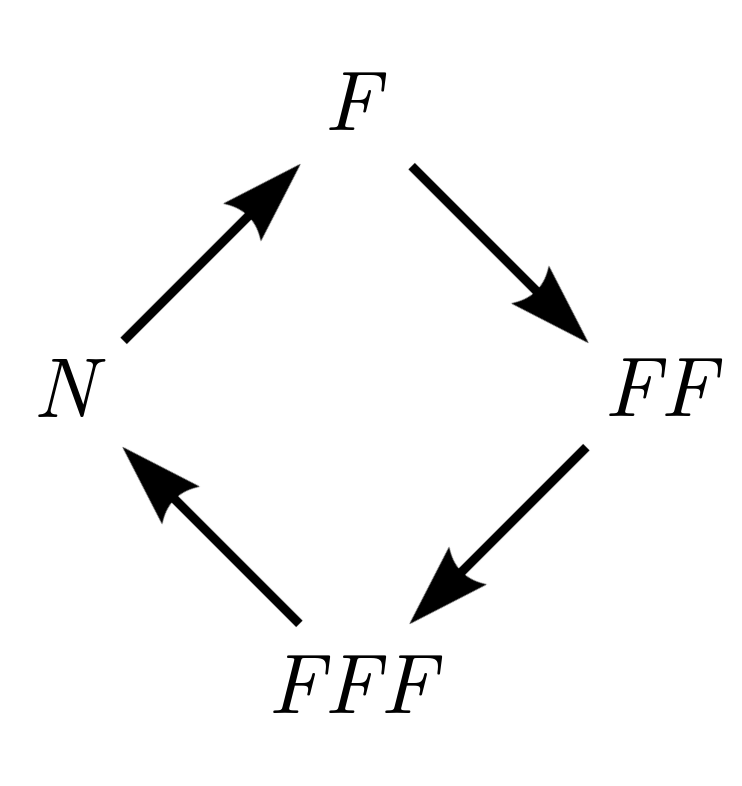
\includegraphics[scale=0.7]{Cayleygraph1.png}
\caption{Cayleygraph zu Erzeuger $\{ F \}$}
\label{27}
\end{figure}

Ein simples Beispiel sieht man in Abbildung \ref{27}: Der Cayleygraph der Untergruppe $F$ von $(\Gtwo, \circ)$, die durch $\{ F \}$  erzeugt wird.
Dieser Cayleygraph ist anschaulich, der er nicht sonderlich komplex ist.
Die Untergruppe wird durch die Ebenendrehung $F$ erzeugt, daraus ergibt sich durch hinzufügen einer weiteren Drehung der vorderen Ebene um $90^\circ$ dann $FF$, dann $FFF$ und dann $FFFF$, was dem neutralen Element $F$ entspricht.


Der Cayleygraph der durch $\{ FF, RR \}$ erzeugten Untergruppe ist etwas komplexer (s. Abbildung \ref{28}). 
Die roten Pfeile repräsentieren den Erzeuger $\{FF\}$ (da es sich dabei in der Startkonfiguration um die rote Seite des Würfels handelt) und die blauen Pfeile repräsentieren den Erzeuger $\{RR\}$ (da es sich dabei um die blaue Würfelseite handelt).
Elemente die durch ein anderes Element in Kombination mit einem Erzeuger entstehen können, sind durch einen Pfeil (Erzeuger) miteinander verbunden.
Die 7 Elemente der durch  $\{ FF, RR \}$ erzeugten Untergruppe sind die Knoten des Graphens. 
Anhand des Cayleygraphens kann man sehen, dass $FFFF$ und $RRRR$ das neutrale Element $N$ ergeben.
Obwohl dieser Cayleygraph wesentlich komplexer ist, als der der Untergruppe $F$ (Abbildung \ref{27}), stellt er eine sehr kleine erzeugte Untergruppe dar, wenn man es mit der Größe der anderen erzeugbaren Untergruppen von $(\Gtwo, \circ)$ vergleicht. Die Untergruppen und Cayleygraphen können bei der Gruppe des \Ttwo Würfels (und des \Tthree Würfels) sehr groß werden.
\begin{figure}[h]
\centering
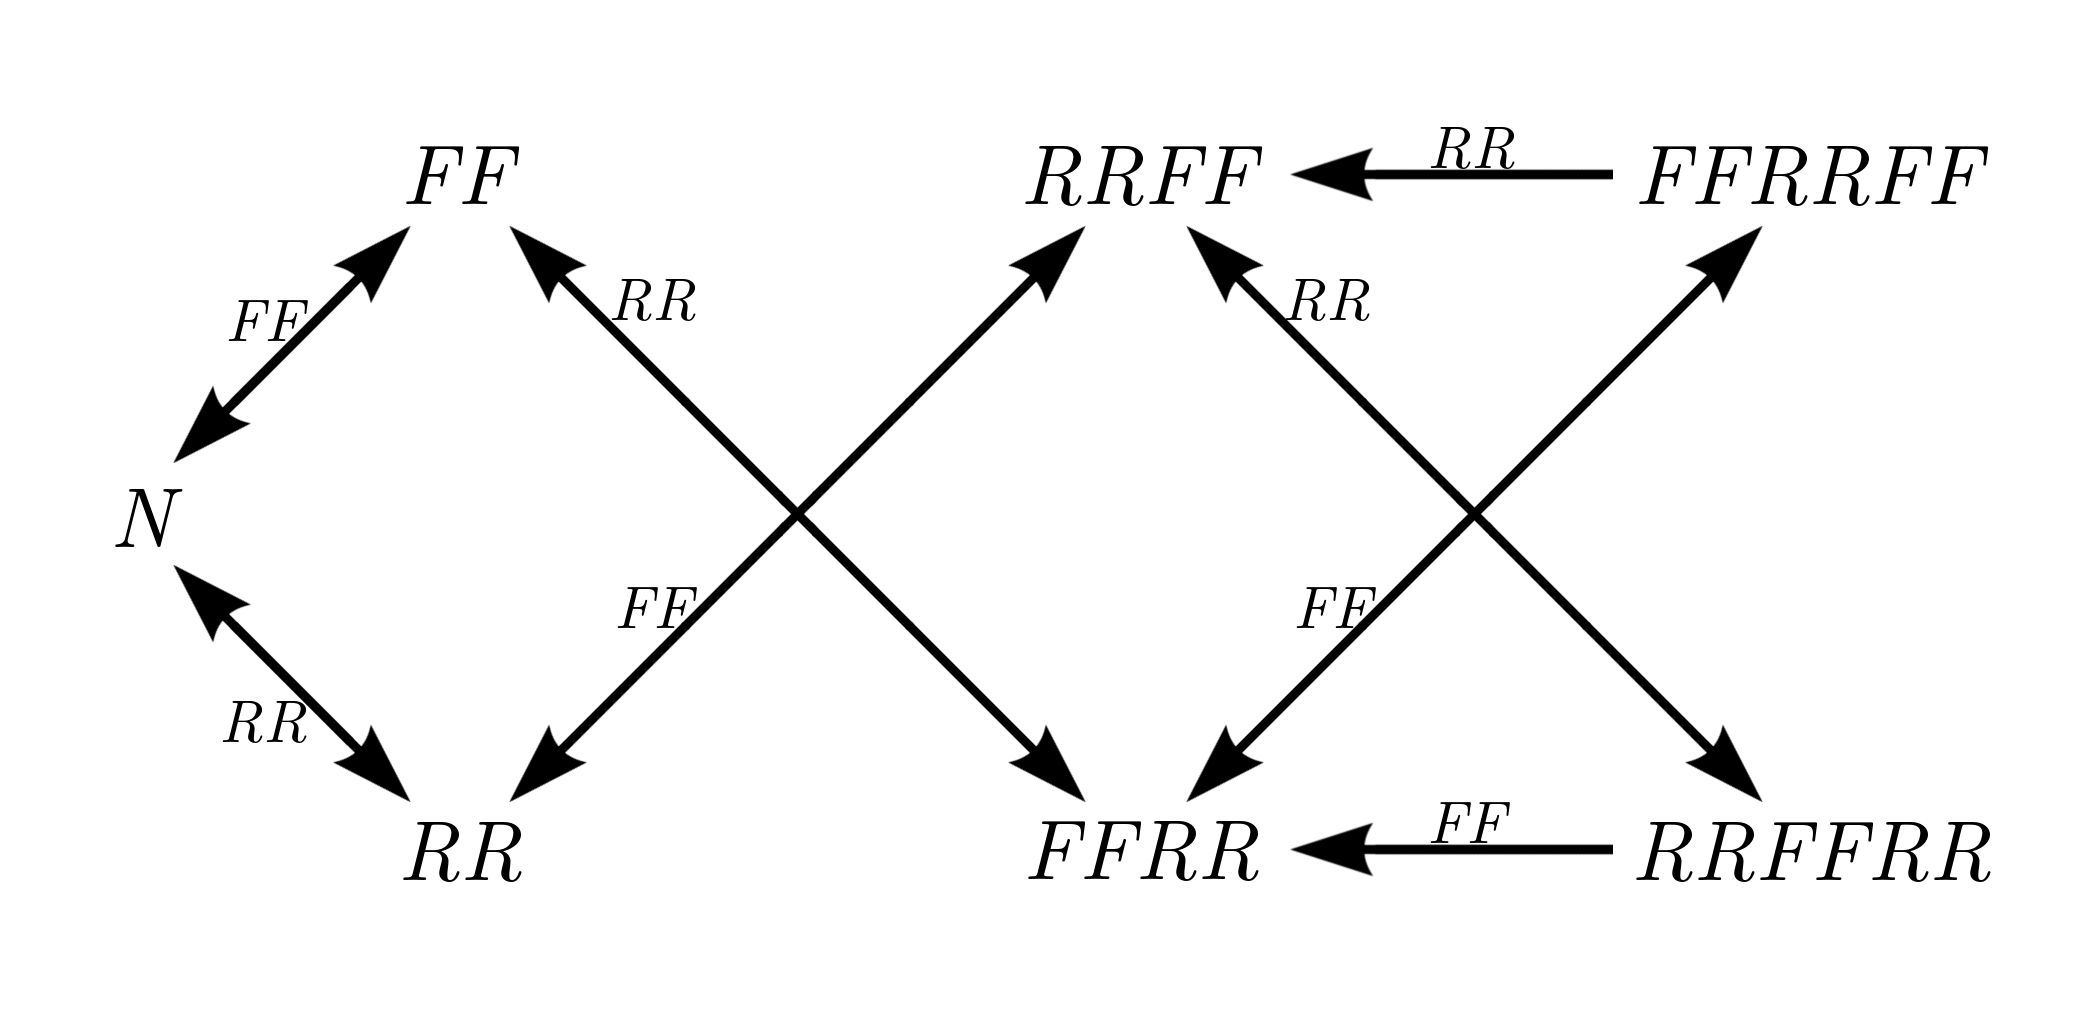
\includegraphics[scale=0.6]{Cayleygraph2.png}
\caption{Cayleygraph zu Erzeuger $\{ FF, RR \}$}
\label{28}
\end{figure}







%
%
%
%
%
%
%
%=======================================================================================================
%
%
%
%
%
%
%
%
%
%
\newpage

\section{Valide Konfigurationen des Würfels}

Nicht jede der theoretisch möglichen Würfelkonfigurationen kann auch wirklich durch Ebenendrehungen erreicht werden. Wie viele Möglichkeiten es im \Ttwo Würfel gibt und welche davon man wirklich erreichen kann, wird im Folgenden berechnet. 
Dazu wird zuerst die Anzahl der theoretisch möglichen Würfelkonfigurationen berechnet:
Die Ecksteine können sich in jeder Ecke befinden, also gibt es pro Eckstein 8 mögliche Positionen im Würfel. Da es 8 Ecksteine gibt, gibt es also $8! = 1 \cdot 2 \cdot 3 \cdot 4 \cdot 5 \cdot 6 \cdot 7 \cdot 8 = 40\, 320$ mögliche Positionen für die Ecksteine.
Außerdem können die Ecksteine gedreht sein, also verschiedene Farbflächen oben sein. Da die Steine aus 3 Farbflächen bestehen, können sieben davon durch Ebenendrehungen theoretisch 3 verschiedene Ausrichtungen annehmen. Der achte Stein kann durch die Möglichkeit der Rotation des kompletten Würfels als richtig gedreht angenommen werden. Es gibt also $3^7$ Wege, wie die Ecksteine ausgerichtet sein können.
Da es keine Mittelsteine im Würfel gibt, reduziert die Rotation des Würfels die Möglichkeiten um den Faktor 24. 
Somit ergibt es $(3^7 \cdot 8!) \cdot \frac{1}{24}$ mögliche Positionen für den Würfel. Das sind $3\, 674\, 160$ Positionen.

Die theoretische Obergrenze der Würfelkonfigurationen liegt bei $8! \cdot 3^8 = 264 \, 539 \, 520$ \cite{MMFAA}. Wenn man nun die Rotation des Würfels berücksichtig kommt man auf $11 \, 022 \, 480$ theoretische Würfelkonfigurationen.
Davon sind aber nicht alle Konfigurationen durch Ebenendrehungen erreichbar -- für einige braucht man einen Schraubendreher oder Superkleber. Diese Konfigurationen werden hier als ungültige Konfigurationen bezeichnet. 
Es sind also nur $\frac{1}{3}$ der Würfelkonfigurationen valide.
%
%
%
%
%
%
%
%
%
%
%=======================================================================================================
%
%
%
%
%
%
%
%
%
%
\subsection*{Ausrichtung der Steine (modulo 3)}\addcontentsline{toc}{subsection}{\protect\numberline{}Ausrichtung der Steine (modulo 3)}

Die Konfiguration des Würfels ist definiert als $C=(\sigma, x)$. In diesem Abschnitt wird gezeigt, dass bei einer validen Würfelkonfiguration \begin{displaymath}
\sum_{i= 1}^{8} \ x_i \mod 3 = 0 
\end{displaymath}  (modulo) gilt. 

Wenn $C'=(\sigma', x')$ eine Nachfolgekonfiguration von der Konfiguration $C=(\sigma, x)$ ist, dann gilt  ${(\sigma, x) \cdot M = (\sigma', x')}$. Dabei ist $M$ eine der Züge aus $U, D, R, L, F, B$. Es gilt dann ${\sum_{i= 1}^{8} \ x_i' \mod 3 = \sum_{i= 1}^{8} \  x_i \mod 3 }$.

In Abbildung \ref{7} kann ist diese Situation für den Zug $R$ dargestellt. Das kann man auch anhand dieser Tabelle sehen: 
\begin{center}
\begin{small}
\begin{tabular}{cllcc}
\toprule
{\footnotesize \textbf{Zug} $\boldsymbol{M}$} & $\boldsymbol{x}$ & $\boldsymbol{x'}$ & {\footnotesize $\boldsymbol{\sum_{i= 1}^{8} x_i'}$} & {\footnotesize $\boldsymbol{\sum_{i= 1}^{8}x_i'\mod 3}$} \\
\midrule
\textit{D} & $(x_1, x_2, x_3, x_4, x_5, x_6, x_7, x_8)$ & $(x_1, x_2, x_3, x_4, x_6, x_8, x_5, x_7)$ & 0 & 0 \\

\textit{U} & $(x_1, x_2, x_3, x_4, x_5, x_6, x_7, x_8)$ & $(x_3, x_1, x_4, x_2, x_5, x_6, x_7, x_8)$ & 0 & 0 \\

\textit{R} & $(x_1, x_2, x_3, x_4, x_5, x_6, x_7, x_8)$ & $(x_1, 2, x_3, 1, x_5, 1, x_7, 2)$ & 6 & 0 \\

\textit{L} & $(x_1, x_2, x_3, x_4, x_5, x_6, x_7, x_8)$ & $(1, x_2, 2, x_4, 2, x_6, 1, x_8)$ & 6 & 0 \\

\textit{F} & $(x_1, x_2, x_3, x_4, x_5, x_6, x_7, x_8)$ & $(x_1, x_2, 1, 2, x_5, x_6, 2, 1)$ & 6 & 0 \\

\textit{B} & $(x_1, x_2, x_3, x_4, x_5, x_6, x_7, x_8)$ & $(2, 1, x_3, x_4, 1, 2, x_7, x_8)$ & 6 & 0 \\
\bottomrule

\end{tabular}
\end{small}

\end{center}
Für jede valide Würfelposition gilt also ${\sum_{i = 1}^{8} \ x_i' \mod 3 = \sum_{i = 1}^{8} \  x_i \mod 3 }$. 
Wenn es also eine valide Konfiguration $C'=(\sigma', x')$, für die gilt $\sum_{i = 1}^{8} x_i' \mod 3 = 0$, dann gibt es einen Zug $M \in \Gtwo$, so dass $M \cdot C'$ die Steine in die richtigen Positionen bringt also $(1,x)$. 
Von dieser Konfiguration $(1,x)$ ausgehend gibt es einen Zug $M \in \Gtwo$, so dass alle Eckstücke richtig ausgerichtet sind. Dann ergibt sich die Konfiguration $(1, 0)$ und alle Eckstücke sind in der richtigen Ausrichtung und Position. Der Würfel befindet sich also in der Startkonfiguration. 
%
%
%
%
%
%
%
%
%
%
%=======================================================================================================
%
%
%
%
%
%
%
%
%
%
\newpage


\section{Lösung des Würfels}

Die übliche, händische Methode zum Lösen eines Zauberwürfels ist das Kombinieren verschiedener Ebenendrehungen. Diese werden als eine Einheit angewendet und verändern den Würfel dann sehr spezifisch. 
Es gibt beispielsweise eine Kombination, die 3 der 4 Ecken der oberen Ebene untereinander im Uhrzeigersinn tauscht und deren Ausrichtung dabei nicht verändert. 

In diesem Kapitel wird die Parität der Züge beschrieben und Kommutatoren erklärt.
Dann wird beispielhaft ein Lösungsvorgang eines Menschens schrittweise beschrieben und erklärt.
Außerdem werden \textit{hübsche} Muster des Würfels algorithmisch beschrieben und gezeigt.
Danach werden verschiedene Lösungsalgorithmen des \Tthree \textit{Cubes} auf den \Ttwo Würfel übertragen.

%
%
%
%
%
%
%
%
%
%
%=======================================================================================================
%
%
%
%
%
%
%
%
%
%
\subsection*{Parität}\addcontentsline{toc}{subsection}{\protect\numberline{}Parität}

Jeder $n$-Zykel kann als Produkt von $2$-Zykeln geschrieben werden. Wenn $n$ dabei gerade ist, hat das dazugehörige $2$-Zykel-Produkt eine ungerade Anzahl an $2$-Zykeln und anders herum. \cite{TD}
Jede Würfelposition kann durch die Ebenendrehungen $U, D, F, B, L, R$ (und die Rotation des Würfels) erreicht werden. 
Zur Erinnerung: Die Ebenendrehungen des Würfels sind durch folgende Zykel definiert:
\begin{align*}
\sigma_U & =\ (ulf \ ulb \ urb \ urf) \\
\sigma_D & =\ (dlf \ drf \ drb \ dlb) \\
\sigma_F & =\ (ulf \ urf \ drf \ dlf) \\
\sigma_B & =\ (ulb \ dlb \ drb \ urb) \\
\sigma_L & =\ (ulb \ ulf \ dlf \ dlb) \\
\sigma_R & =\ (urb \ drb \ drf \ urf) \\
\end{align*}
Jeder Zug ist also als ein $4$-Zykel definiert. Den $4$-Zykel kann man als Produkt aus drei $2$-Zykeln schreiben. 
Die Parität einer einzelnen Ebenendrehung ist also ungerade. Die Parität eines Zuges, der aus zwei Ebenendrehungen besteht (z.B. $LF$) ist somit gerade.

% to do prüfen! 

%
%
%
%
%
%
%
%
%
%
%=======================================================================================================
%
%
%
%
%
%
%
%
%
%
\subsection*{Kommutatoren}\addcontentsline{toc}{subsection}{\protect\numberline{}Kommutatoren}

Der Kommutator von zwei Elementen $Y, Z$ der Gruppe $(\Gtwo, \circ)$ ist definiert als $[Y,Z]=YZY^{-1}Z^{-1}$ (s. Kapitel \ref{11}).
Kommutierende Elemente ergeben das neutrale Element einer Gruppe. 
Wenn $Y = Z$ mit $Y, Z \in \Gtwo$ gilt, kommutieren $Y$ und $Z$. 
Dazu folgt nun der Beweis. 

Zur Veranschaulichung wird $[Y,Z]$ mit $Y=Z$ nun als $[Z,Z]$ geschrieben. Das ist dann das Gleiche wie $ZZZ^{-1}Z^{-1} = Z(ZZ^{-1})Z^{-1}$. 
$(ZZ^{-1})$ ist äquivalent mit dem neutralen Element $N$. Daraus ergibt sich $Z(N)Z^{-1} = ZZ^{-1} = N$. 
Somit kommutieren alle $Y, Z \in \Gtwo$ mit $X=Y$.


Es kommutieren auch Züge, die nur gegenüberliegende Ebenen beeinflussen und somit nicht dieselben Steine bewegen. 
Das sind dann die Kommutatoren der Form $[U^n, D^n]$, $[F^n, B^n]$ und $[L^n, R^n]$ mit $n \in \mathbb{N}_0$. 
Da die beiden Züge nicht dieselben Steine beeinflussen, ist es nicht relevant, dass die Gruppe nicht kommutativ ist und durch $YZY^{-1}Z^{-1}$ werden beide Züge wieder invertiert. 


Auch wenn zwei Züge $Y, Z \in \Gtwo$ nicht kommutieren, kann anhand der Komplexität des Kommutators festgestellt werden, wie groß die Veränderung der Würfelkonfiguration nach $[Y, Z]$ ist. 
Als Beispiel zur Veranschaulichung: Die Züge $Y=L$ und $Z=F$ verändern durch $[Y, Z]$ vier Steine im Würfel. Die anderen vier behalten ihre Position und Ausrichtung. 
Es wird also $LFL^{-1}F^{-1}$ ausgeführt. Das führt zu folgenden Permutationen:

\begin{center}
\begin{tabular}{lcccccccc}
\toprule
\textbf{Zug} & \textbf{ulb} & \textbf{urb} & \textbf{ulf} & \textbf{urf} & \textbf{dlb} & \textbf{drb} & \textbf{dlf} & \textbf{drf} \\

\midrule
$L$ & ulf & \textcolor{gray}{urb} & dlf & \textcolor{gray}{urf} & ulb & \textcolor{gray}{drb} & dlb & \textcolor{gray}{drf} \\

$F$ & urf & \textcolor{gray}{urb} & ulf &  drf & \textcolor{gray}{ulb} & \textcolor{gray}{drb} & \textcolor{gray}{dlb} & dlf \\

$L^{-1}$ & \textcolor{gray}{urf} & \textcolor{gray}{urb} & ulb & \textcolor{gray}{drf} & dlb & \textcolor{gray}{drb} & dlf & ulf \\

$F^{-1}$ \: & ulf & \textcolor{gray}{urb} & \textcolor{gray}{ulb} & urf & \textcolor{gray}{dlb} & \textcolor{gray}{drb} & drf & dlf\\
\bottomrule
\end{tabular}
\end{center}

Wenn man nun die Kopfzeile der Tabelle und die unterste Zeile vergleicht, sieht man, dass $urb, urf, dlb$ und $drb$ wieder an ihrer Ausgangsposition sind. Die anderen vier Steine ($ulf, ulb, urf$ und $ulf$) haben die Positionen gewechselt: \\
\\
$ulb \mapsto ulf$ \hspace*{2.5cm }$ulf  \mapsto ulb$ \hspace*{2.5cm } $dlf \mapsto drf$ \hspace*{2.5cm } $drf \mapsto dlf$
\\
\\
(Daraus ergibt sich $\lbrack L, F \rbrack  = (ulb \ ulf)(dlf \ drf)$ in der Zykelschreibweise.)

%
%
%
%
%
%
%
%
%
%
%=======================================================================================================
%
%
%
%
%
%
%
%
%
%
\subsection*{Lösungsansätze}\addcontentsline{toc}{subsection}{\protect\numberline{}Lösungsansätze}
Für die Lösung des Würfels sind Züge nützlich, die nur wenige Steine bewegen. So kann man dann gezielt bestimmte Steine drehen oder tauschen. 

Es gibt verschiedene Vorgehensweisen um den Würfel zu lösen. Üblicherweise fängt man mit der weißen Seite an, deshalb werden auch die folgenden Beispiele so vorgehen. Die gelbe Seite gehört dann zur letzten Ebene, die gelöst wird. 
Für die Lösungsalgorithmen ist die Farbe der ersten Seite nicht relevant. Es wird aber häufig mit weiß begonnen, da man sich die Anordnung der Farben so leichter merken und und schneller sieht, in welche Ebene ein Stein gehört \cite{RF}. 

Eine gängige Lösungsmethode geht so vor, dass bei der letzten Ebene zuerst alle Steine richtig ausgerichtet werden. Dann sind alle $x_i=0$. Danach werden die Positionen noch getauscht. 
Dafür dreht man den Würfel üblicherweise, damit die gelbe Seite oben ist. 
Ein Beispiel für einen Zug dieses Lösungsansatzes ist $\lbrack R, U \rbrack \lbrack R^{-1}, F \rbrack$. Dabei werden zwei Steine der oberen Ebene gedreht und drei Steine verändern ihre Position. Dieser Zug kann für die Lösung der zweiten Ebene genutzt werden, ohne dabei die erste Ebene zu verändern. \cite{RF2} 
In Abbildung \ref{25} sieht man, wie der Würfel bei der Ausgangsposition (links) durch den Zug $\lbrack R, U \rbrack \lbrack R^{-1}, F \rbrack$ verändert wird. Die Steine der oberen Ebene werden dabei ausgerichtet.

\begin{figure}[h]
\centering
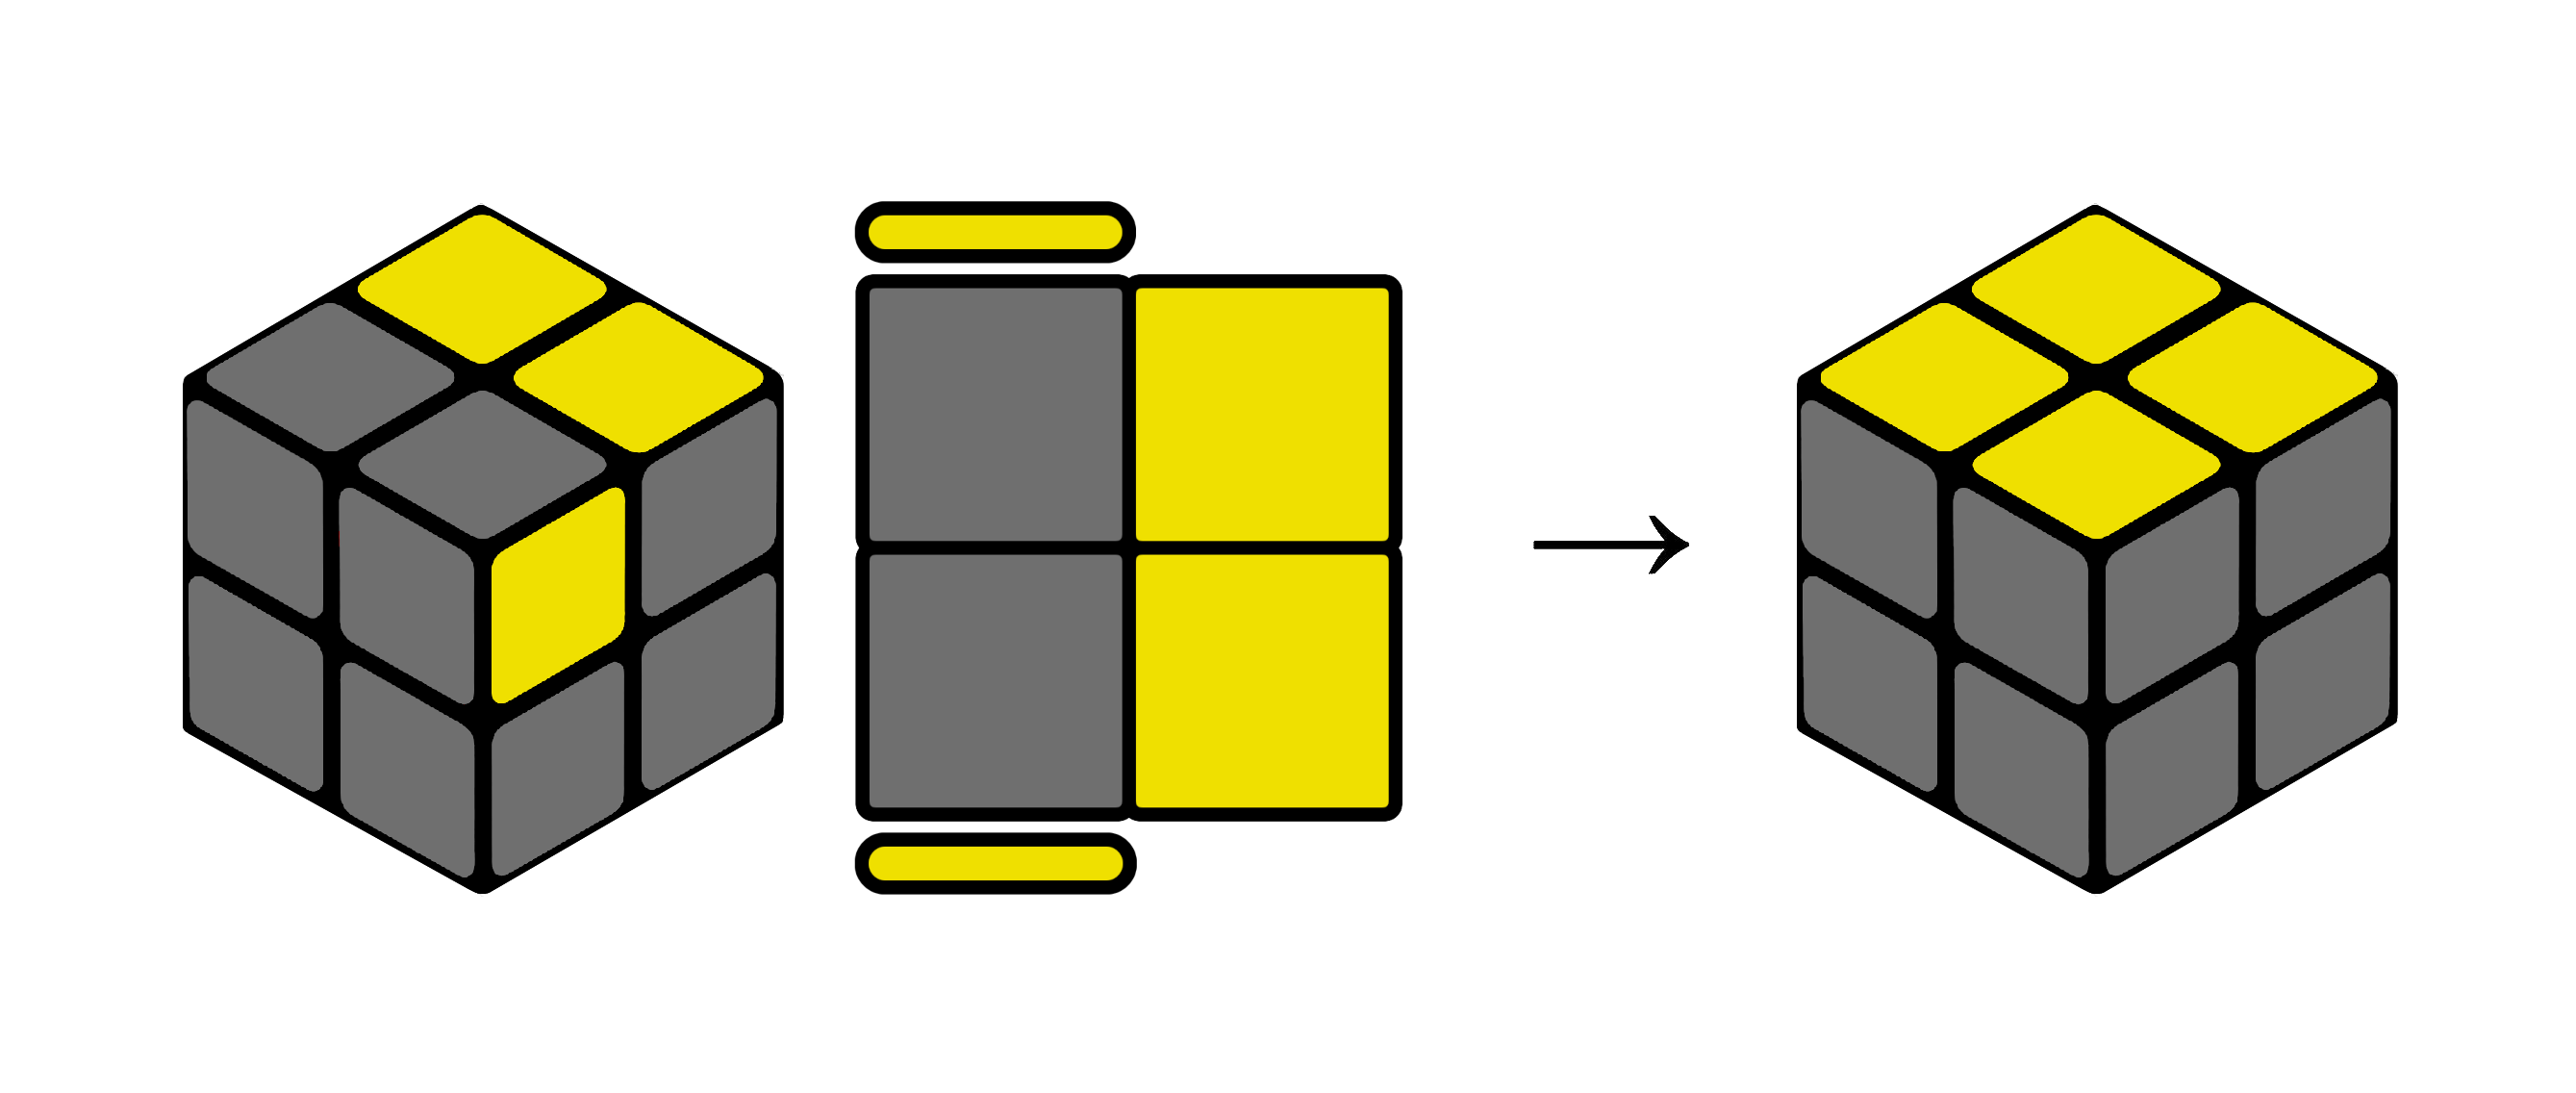
\includegraphics[scale=0.12]{isiakanm.png}
\caption{Ausrichtung der zweiten Ebene (Beispiel)}
\label{25}
\end{figure}

Man kann $\lbrack R, U \rbrack \lbrack R^{-1}, F \rbrack$ auch als Zykel schreiben: $(ulb \ ulf \ urb)$. 
%
%
%
%
%
%
%
%
%
%
%=======================================================================================================
%
%
%
%
%
%
%
%
%
%
\subsection*{Lösung des Würfels anhand eines Beispiels}\addcontentsline{toc}{subsection}{\protect\numberline{}Lösung des Würfels anhand eines Beispiels}

In diesem Beispiel (Abbildung \ref{18}) wird der Würfel mit dem Zug $FUBRF^{-1}$ verdreht und so gelöst, wie ein Mensch den \textit{Cube} lösen würde.
In der Abbildung wurde der Würfel noch um $180^\circ$ um die $z$-Achse rotiert.

\begin{figure}[h]
\centering
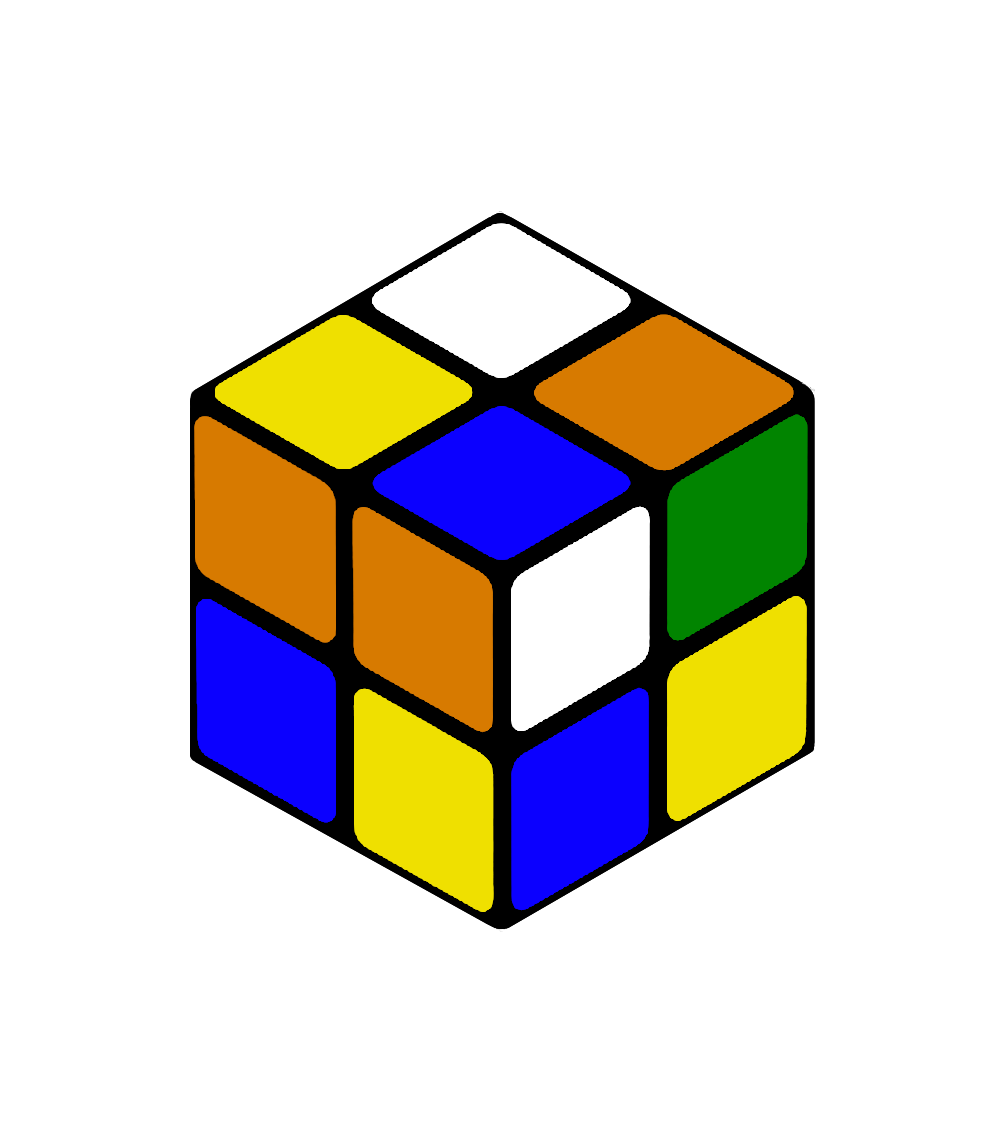
\includegraphics[scale=0.12]{LURFL1.png}
\caption{\textit{Cube} nach Zug $FUBRF^{-1}$ }
\label{18}
\end{figure}

Der erste Schritt für einen menschlichen Ansatz der Lösung des Würfels ist (meistens), die Steine der oberen Ebene so anzuordnen, dass die Farbflächen dort alle weiß sind und die vier oberen Steine in der richtigen Position zueinander sind. 
Es muss also $x_{1-4} = (0,0,0,0)$ gelten und $\sigma_{ulb}=ulb, \sigma_{urb} = urb, \sigma_{ulf} = ulf, \sigma_{urf}=urf$ bzw. die Äquivalenzklassen $\delta_{Z_r}$ und $\delta_{Z_l}$ davon. 

Der Lösende sucht nun also Steine mit weißen Farbflächen und findet den weiß-orange-blauen Stein an der Position $urf$. 
Mit dem Zug $F^{-1}$ findet der Stein seinen Platz in der oberen Ebene, mit der weißen Farbfläche oben. 
Nun ist $x_{1-4}=(0,2,0,1)$ und der Würfel sieht so aus, wie in Abbildung \ref{19} dargestellt: Es befinden sich nun zwei Steine der oberen Ebene an der richtigen Position -- der weiß-orange-blaue Stein und der weiß-rot-blaue Stein.

\begin{figure}[h]
\centering
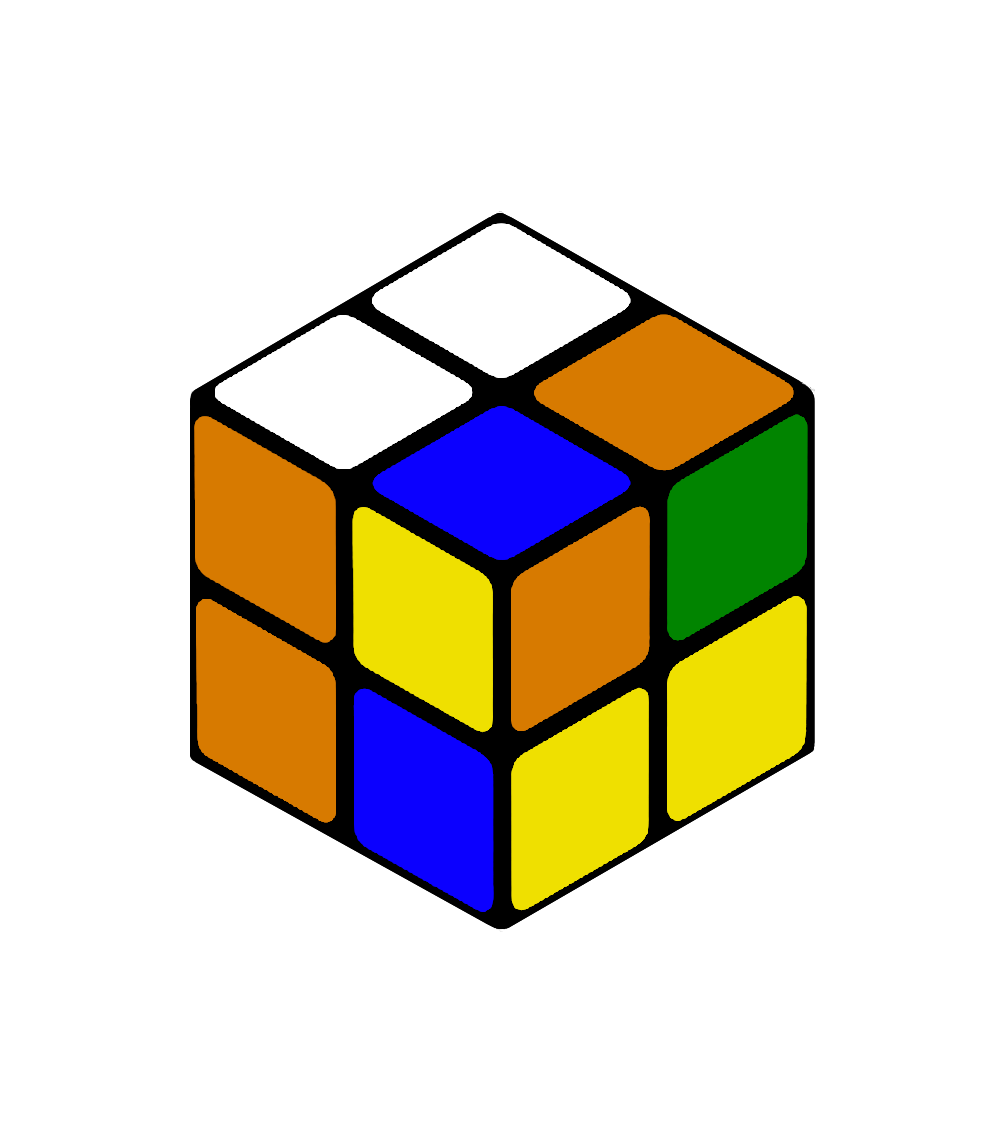
\includegraphics[scale=0.12]{0201.png}
\caption[Lösung von Mensch: Schritt 1]{Lösung von Mensch: Schritt 1}
\label{19}
\end{figure}

Der nächste Stein, der angeordnet wird, ist hier der weiß-grün-orange Stein. Er wird durch den Zug $R^{-1}$ in Position gebracht und findet seinen Platz neben dem weiß-orange-blauen Stein in der oberen Ebene (s. Abbildung \ref{20}).
 
\begin{figure}[h]
\centering
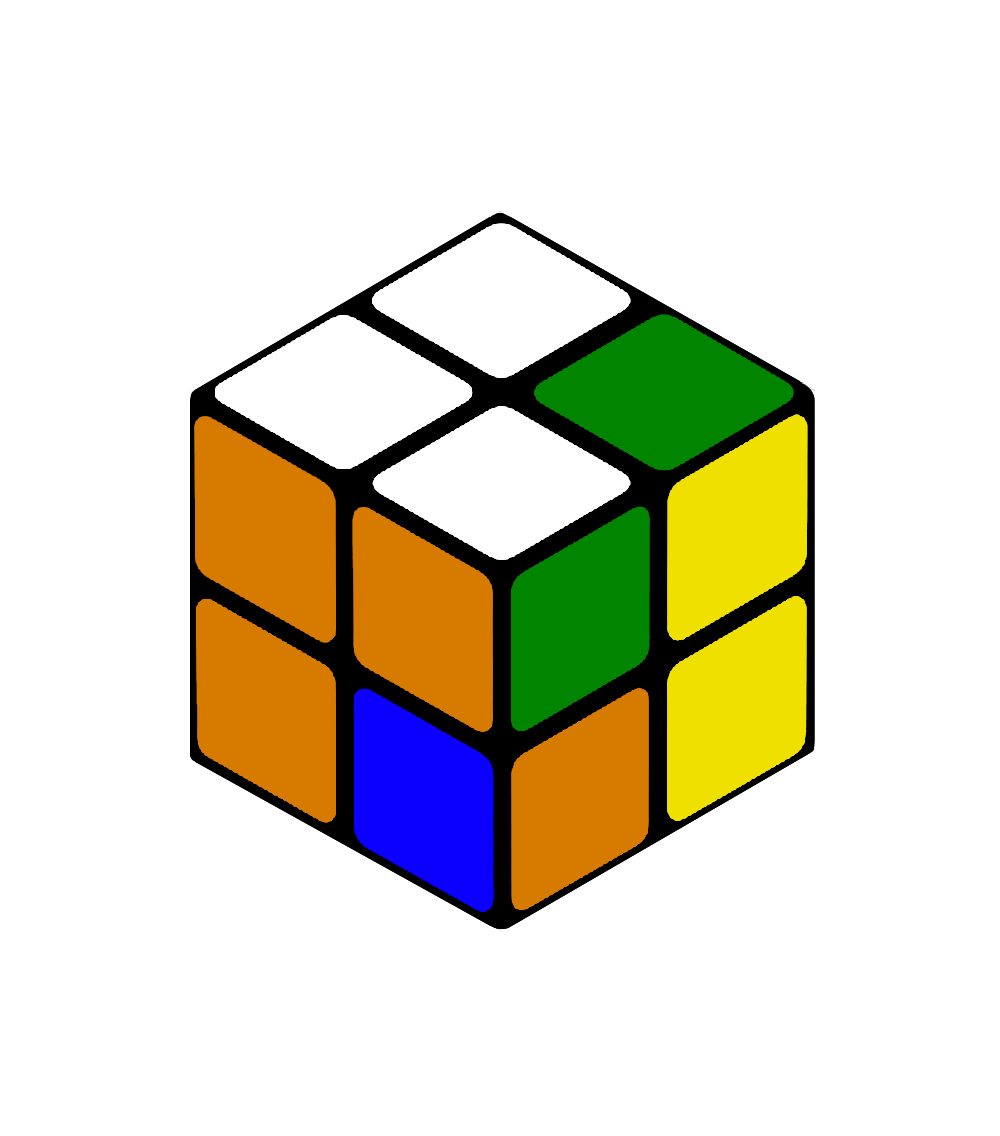
\includegraphics[scale=0.12]{menschSchritt2.png}
\caption[Lösung von Mensch: Schritt 2]{Lösung von Mensch: Schritt 2}
\label{20}
\end{figure}

Der letzte Stein mit weißer Farbfläche wird dann durch den Zug $RD^{-1}R^{-1}$ positioniert. Die obere Ebene ist nun gelöst und alle Steine mit weißen Farbflächen sind wie in der Startkonfiguration zueinander ausgerichtet. (s. Abbildung \ref{21}).
Also gilt $x_{1-4} = (0,0,0,0)$ und durch die Äquivalenzklassen $\delta_{Z_r}$ oder $\delta_{Z_l}$ kann man sehen, dass die Steine der oberen Ebene richtig zueinander angeordnet sind. Sie sind aber um $180^\circ$ gedreht zur Startkonfiguration. 

\begin{figure}[H]
\centering
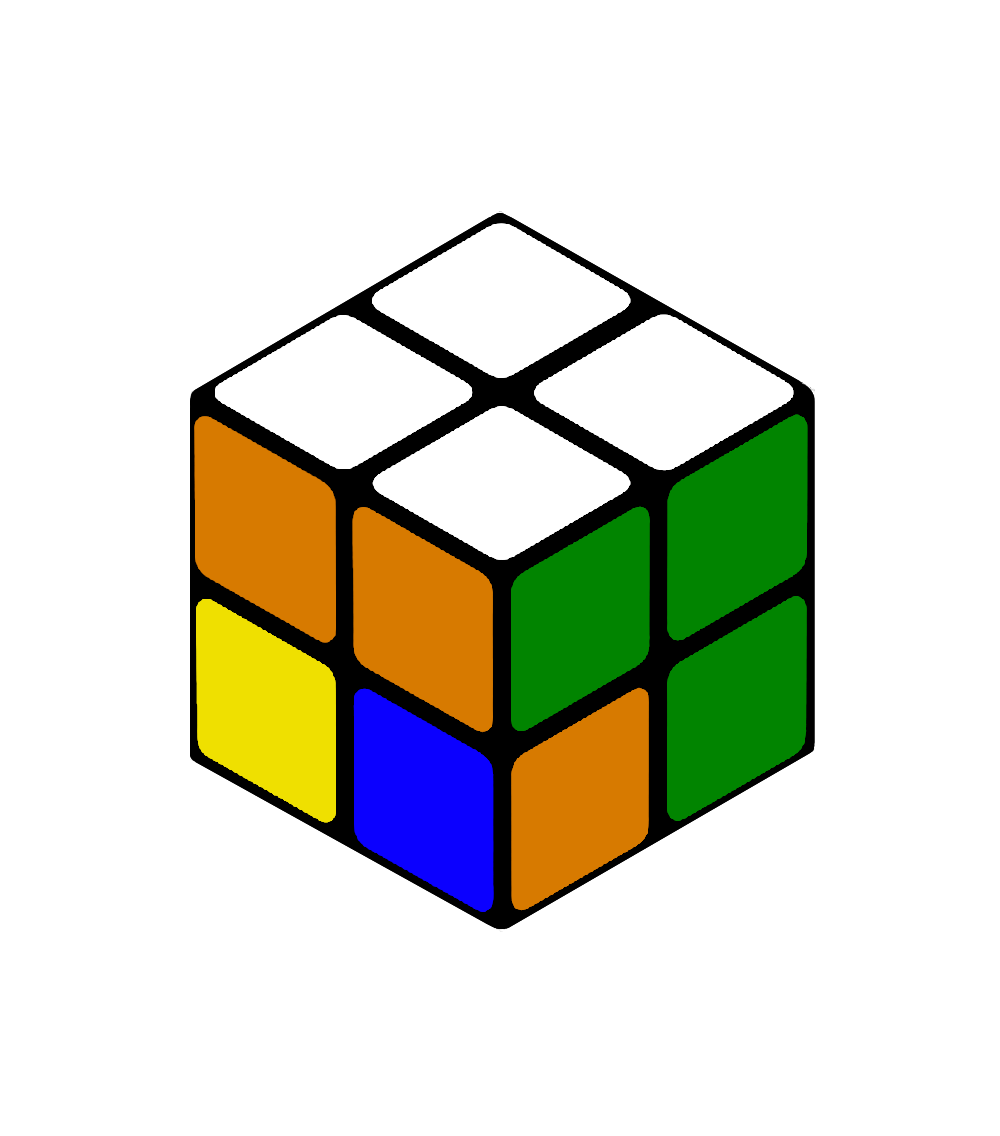
\includegraphics[scale=0.12]{menschSchritt3.png}
\caption[Lösung von Mensch: Schritt 3]{Lösung von Mensch: Schritt 3}
\label{21}
\end{figure} 

Für den nächsten Schritt rotiert der Mensch den Würfel, hier um die $y$-Achse (s. Abbildung \ref{22}). Die weiße Seite ist nun unten und zwei der vier gelben Farbflächen sind nach oben ausgerichtet.

\begin{figure}[H]
\centering
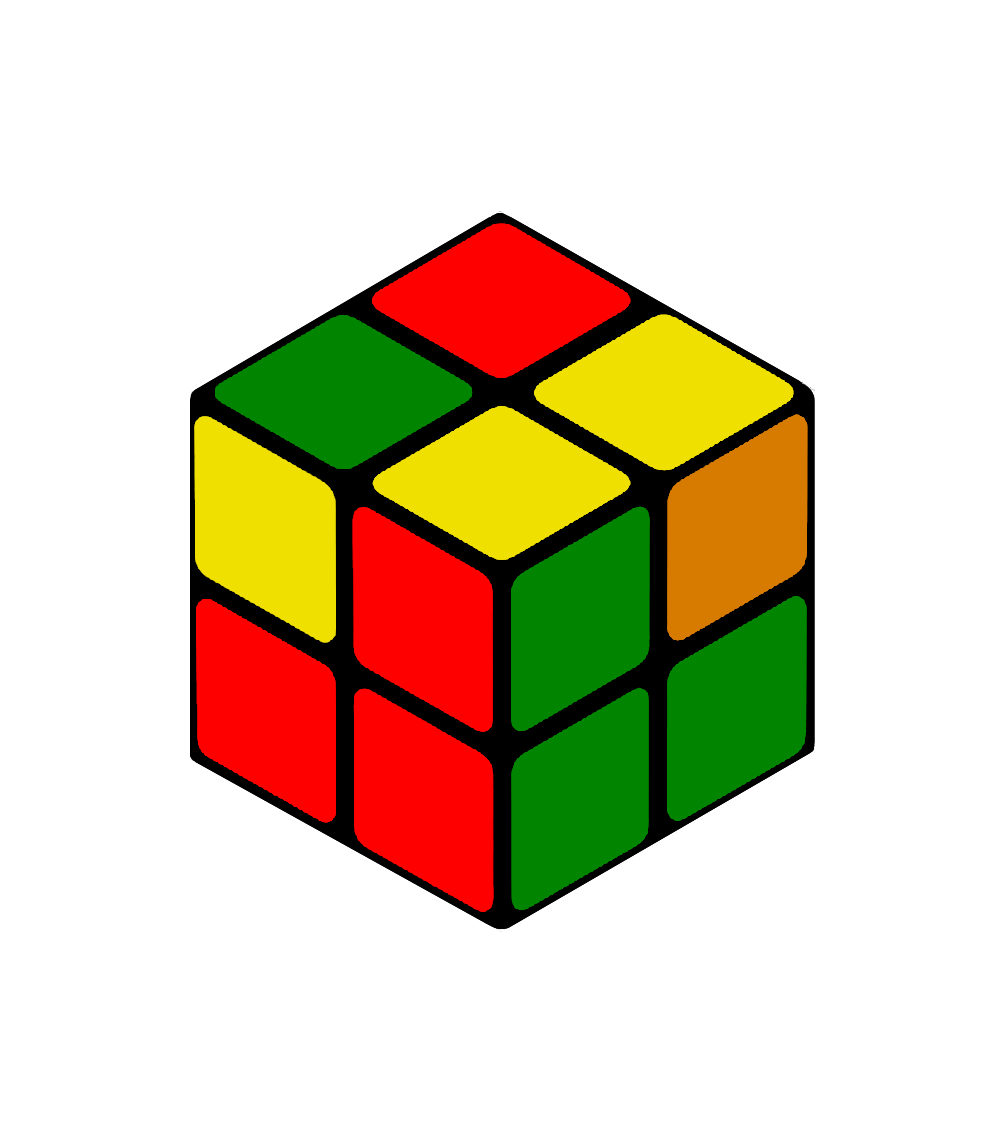
\includegraphics[scale=0.12]{menschSchritt4.png}
\caption[Lösung von Mensch: Schritt 4]{Lösung von Mensch: Schritt 4}
\label{22}
\end{figure} 

Dann führt der Lösende den Zug $RUR^{-1}U^{-1} \ R^{-1}FRF^{-1}$ aus \cite{RF2} und erhält einen gelösten Würfel (s. Abbildung \ref{23}). 

\begin{figure}[H]
\centering
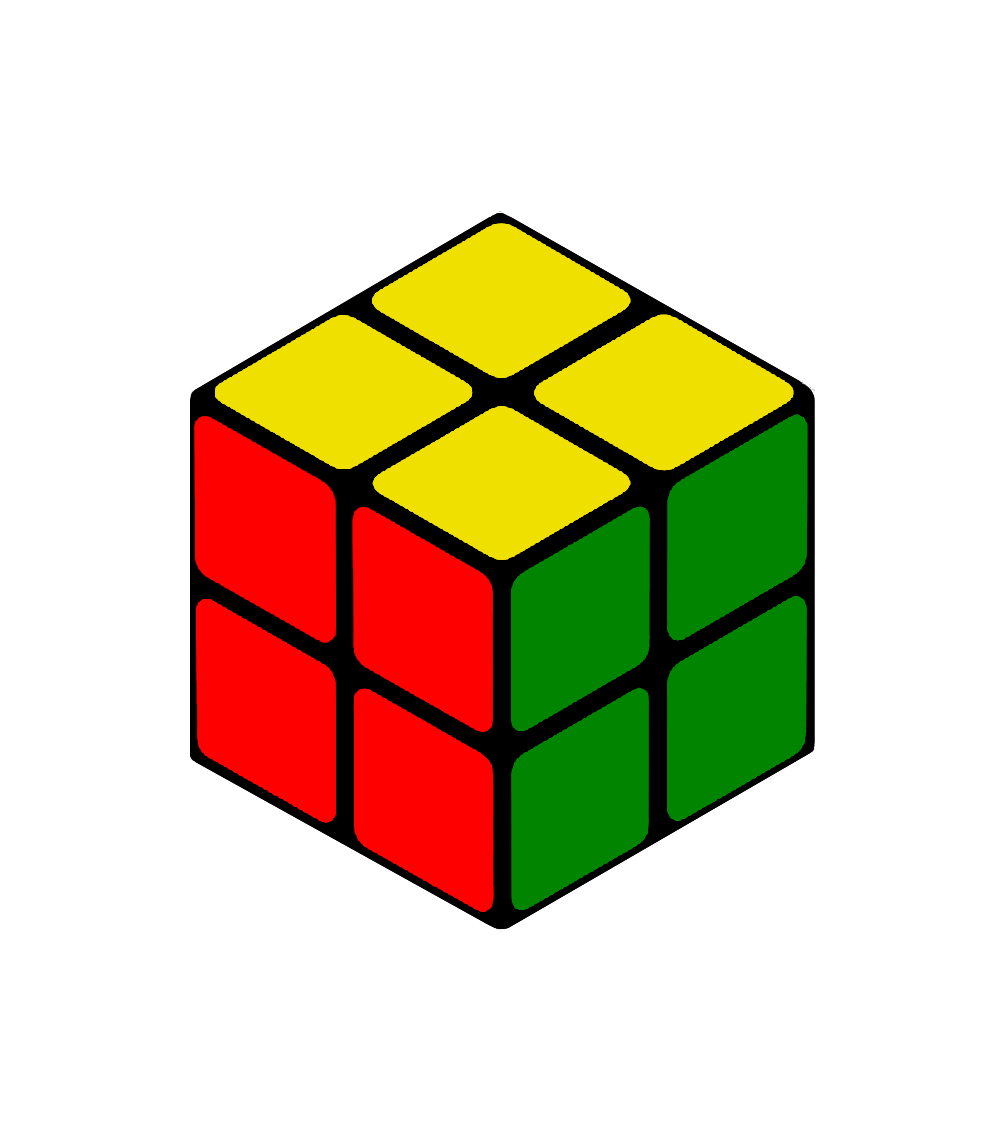
\includegraphics[scale=0.12]{menschSchritt5.png}
\caption[Lösung von Mensch: Schritt 5]{Der \textit{Cube} ist gelöst, die weiße Seite ist unten.}
\label{23}
\end{figure}

Der Mensch folgt beim Lösen des \textit{Cubes} (meistens) bestimmten Kombinationen, die man in verschiedenen Situtionen anwenden kann.  
In diesem Fall hat der Mensch $13$ Ebenen gedreht, während das Verdrehen nur $5$ Ebenenrotationen benötigte. Der Mensch hat also nicht den kürzesten Weg gewählt, aber dafür einen Weg, den er bei verschiedenen Würfelkonfiguratonen anpassen und verwenden kann. 
Wenn man die Verdrehung des Würfels invertiert, also $(FUBRF^{-1})^{-1}$ erhält man die Kombination $FR^{-1}B^{-1}U^{-1}F^{-1}$, um den Würfel zu lösen.


Es stellt sich die Frage, wie viele Ebenendrehungen der \Ttwo Würfel maximal von der Lösung entfernt sein kann. Diese Zahl wird auch \textit{God's Number} genannt. \\
Wenn man davon ausgeht, dass jede $90^\circ$-Drehung einer Ebene als Drehung gezählt wird (und $180^\circ$-Drehungen als zwei Drehungen), ist die \textit{God's Number} des Würfels $14$. \cite{DJ} 


%
%
%
%
%
%
%
%
%
%=======================================================================================================
%
%
%
%
%
%
%
%
%
%
\subsection*{Hübsche Muster}\addcontentsline{toc}{subsection}{\protect\numberline{}Hübsche Muster}
Dieser Abschnitt ist inspiriert von dem Part \textit{Pretty Patterns} in Tom Davis Paper \textit{Group Theory via Rubik's Cube} \cite{TD}.
Dort zeigt er einige \textit{hübsche} Muster des \Tthree Würfels und hier werden nun einige Muster des \Ttwo Würfels gezeigt.
In Abbildung \ref{29} werden vier Muster des \textit{Cubes} gezeigt und die dazugehörigen Algorithmen von der Startkonfiguration ausgehend beschrieben.

\begin{figure}[h]
\centering
\begin{tabular}{cc}
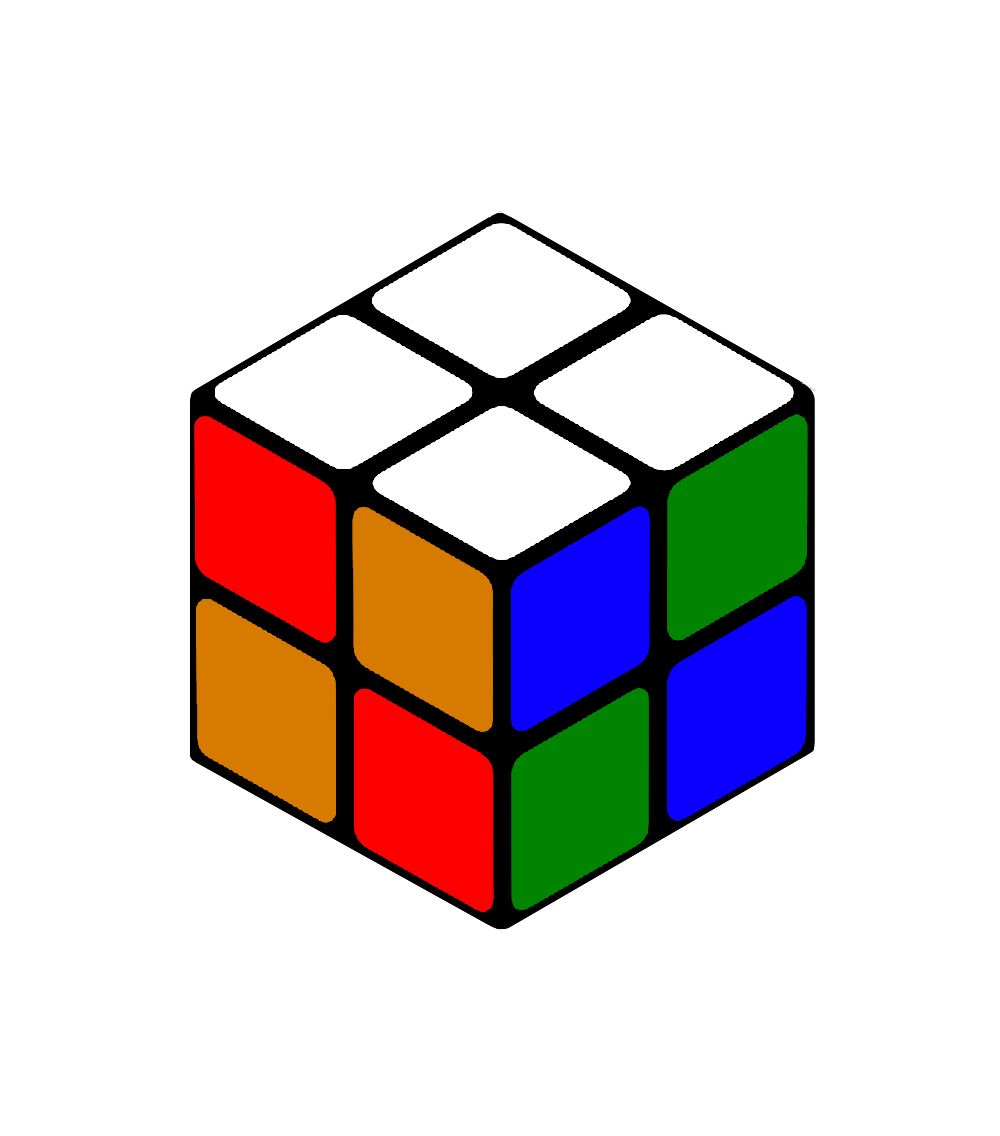
\includegraphics[scale=0.1]{RRFFRRUU.png} &  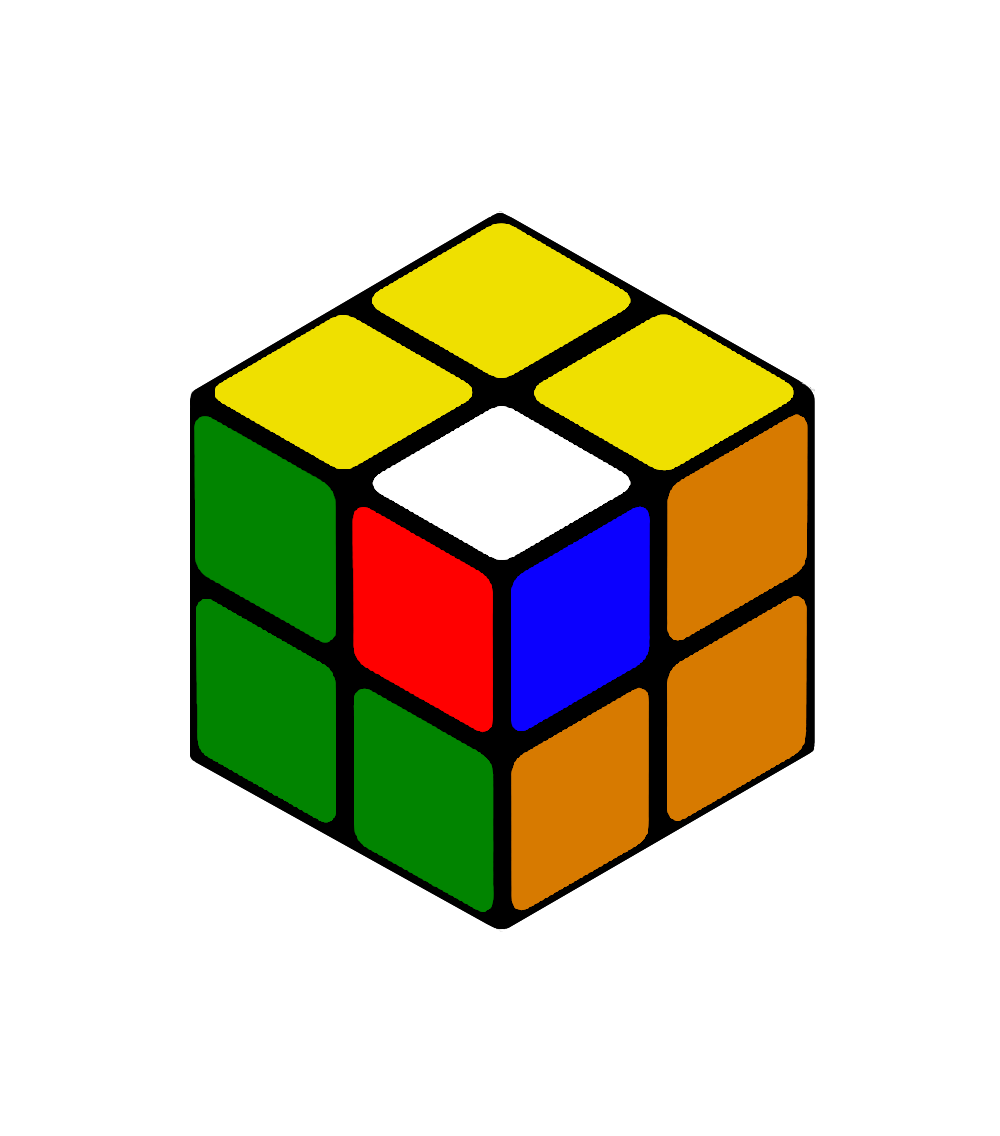
\includegraphics[scale=0.1]{CubeInCube.png} \\
Muster 1 & Muster 2 \\
$RR \ FF \, RR \ UU$ &  $R \ F \, U^{-1} \, RR \ U \, F^{-1} \, R \ U \, FF \, RR$ \\
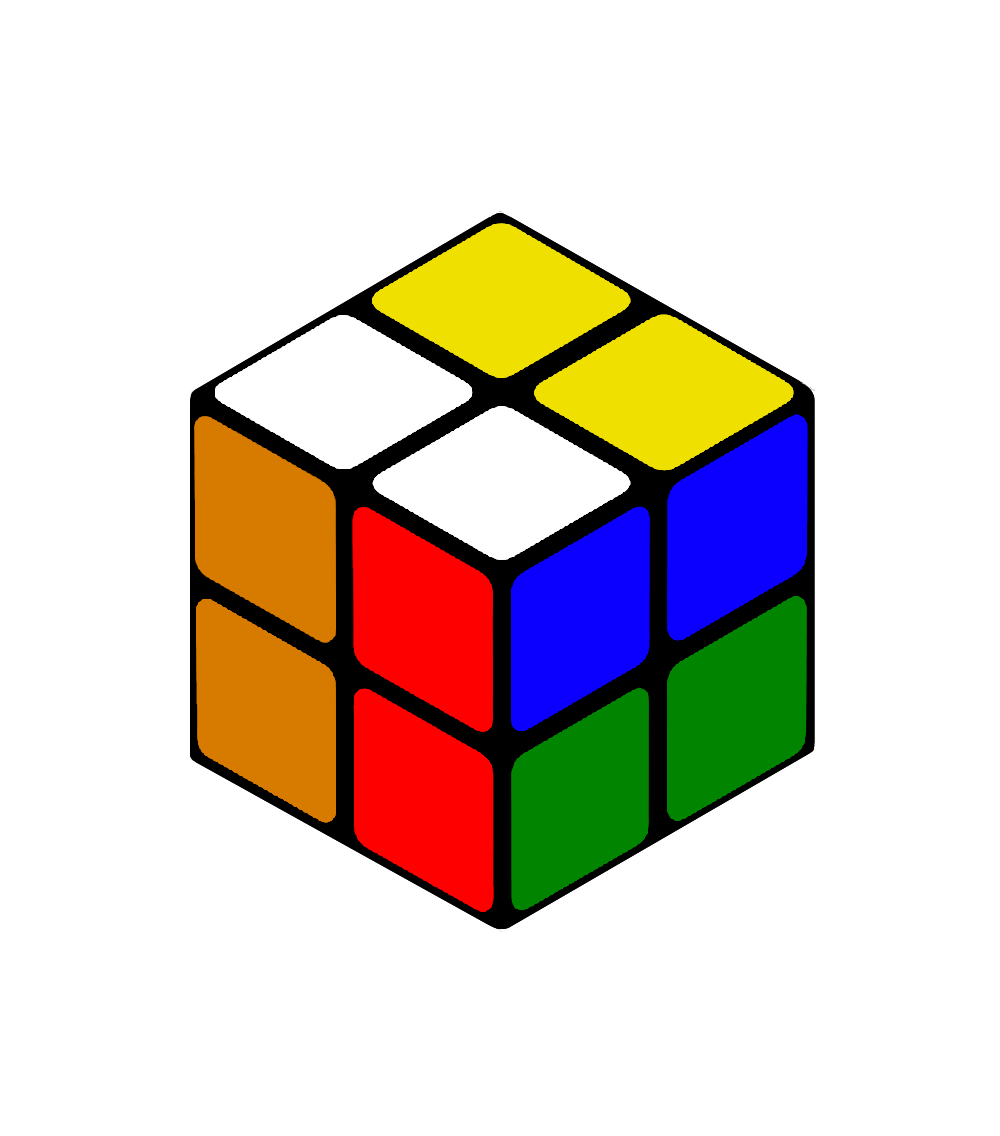
\includegraphics[scale=0.1]{UUFFRRUU.png} &  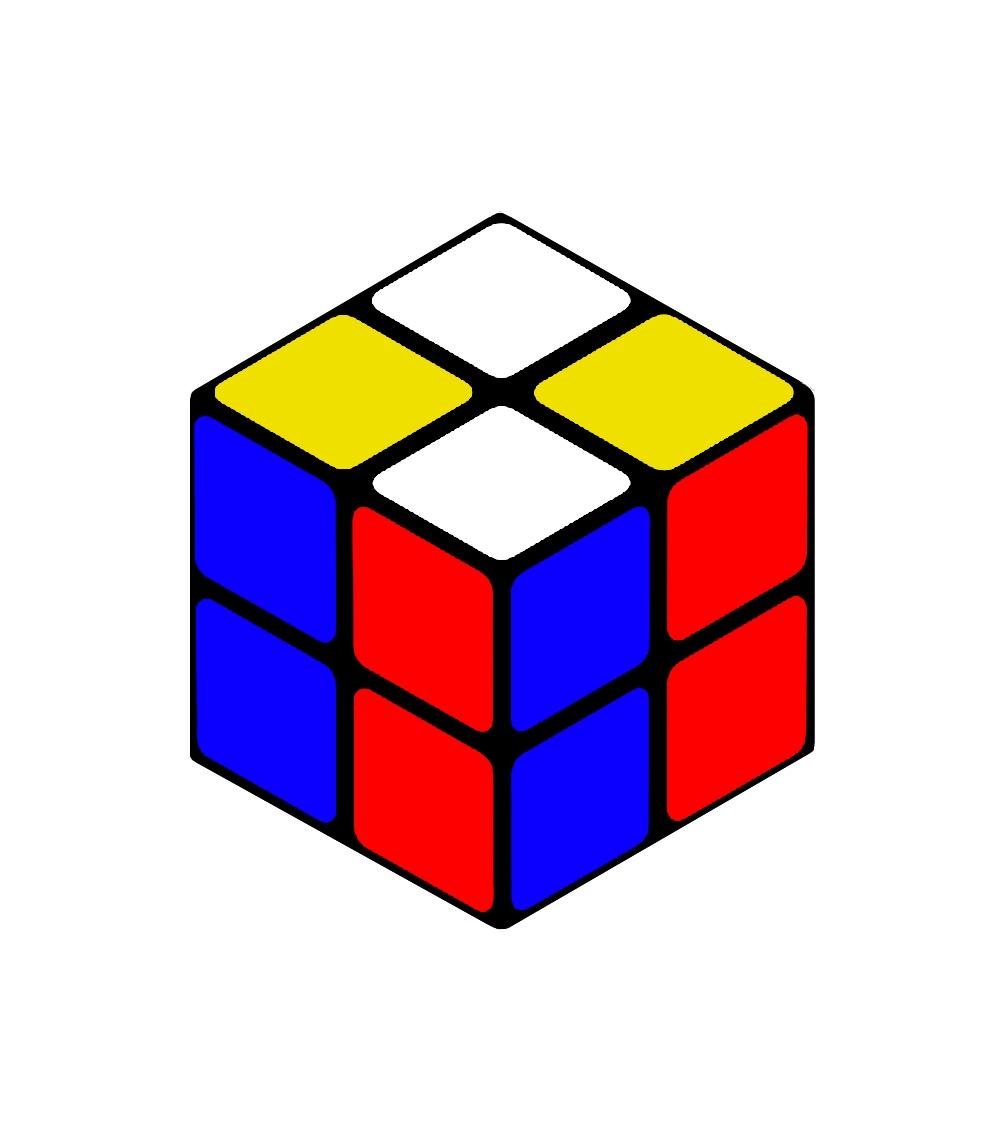
\includegraphics[scale=0.1]{UFFUURRU.png} \\
Muster 3 & Muster 4 \\
$UU \, FF \, RR \ UU$ &  $U \, FF \, UU \, RR \ U$ \\
\end{tabular}

\caption{\textit{Hübsche} Muster des \Ttwo Würfels}
\label{29}
\end{figure}

Muster 1 lässt die weiße und gelbe Seite unverändert und bildet ein Karomuster auf den anderen vier Seiten. Dabei werden die Farbpaare rot-orange und grün-blau zusammen im  Karomuster angeordnet.

Muster 2 hat einen \textit{Würfel im Würfel}. Dabei werden zwei Steine getauscht, die keine gemeinsame Farbfläche haben.

Muster 3 zeigt abwechselnd Quer- und Längsstreifen auf den verschiedenen Seiten.

Muster 4 ordnet die Farben wie vier Säulen an. Die weiße und die gelbe Seite ist dabei kariert, die anderen Seiten gestreift.


Diese Muster sind in den meisten Fällen zwar keine üblichen Lösungsalgorithmen, sollten aber in dieser Arbeit auch nicht unerwähnt bleiben.

%
%
%
%
%
%
%
%
%
%=======================================================================================================
%
%
%
%
%
%
%
%
%
%
\subsection*{Schraubendrehermethode}\addcontentsline{toc}{subsection}{\protect\numberline{}Schraubendrehermethode}

Die Methode, die oft als einfachste Methode zum Lösen von Zauberwürfeln beschrieben wird, ist die Schraubendrehermethode.
Bei den üblichen \Ttwo Würfel kann man auf einer oder mehreren Seiten in der Mitte zwischen den Steinen eine Schraube sehen.
Um den Würfel auseinander zu bauen, muss man diese Schrauben lockern. Daraufhin kann man die Ebene ohne Probleme abnehmen. 
Dann kann man die Steine neu arrangieren und den Würfel in der gelösten Konfiguration wieder zusammen bauen.

Ob das wirklich die einfachste Methode ist, liegt wohl im Auge des Betrachters und wenn man die Tatsache berücksichtigt, dass der Weltrekord des \Ttwo Würfels mit der Methode des algorithmischen, händischen Lösens bei $0,49$ Sekunden liegt \cite{rekord}, ist die Schraubendrehermethode wohl kaum die schnellste Methode.

%
%
%
%
%
%
%
%
%
%=======================================================================================================
%
%
%
%
%
%
%
%
%
%
\subsection*{Algorithmen für die erste Ebene}\addcontentsline{toc}{subsection}{\protect\numberline{}Algorithmen für die erste Ebene}


Da der \Ttwo im Gegensatz zum \Tthree Würfel keine Mittelsteine hat, kann der erste Eckstein als richtig angenommen werden, da man dazu den Würfel nur drehen muss, um eine weiße Farbfläche zu finden.
In diesen Beschreibungen wird sich an die Konvention gehalten, mit der weißen Seite oben zu beginnen. Man kann aber natürlich mit jeder anderen Seite des Würfels auch beginnen.
Den \Tthree \textit{Cube} muss man entsprechend der Mittelsteine ausrichten und so ist vorbestimmt, welche Seite die weiße Seite wird. Bei dem \Ttwo \textit{Cube} kann man mit jeder beliebigen Seite beginnen. Möchte man aber unbedingt mit einer bestimmten Seite beginnen, die noch keine weiße Farbfläche hat, so kann man die Farbfläche durch maximal zwei Ebenendrehungen an diese Seite bringen.

\begin{figure}[h]
\centering
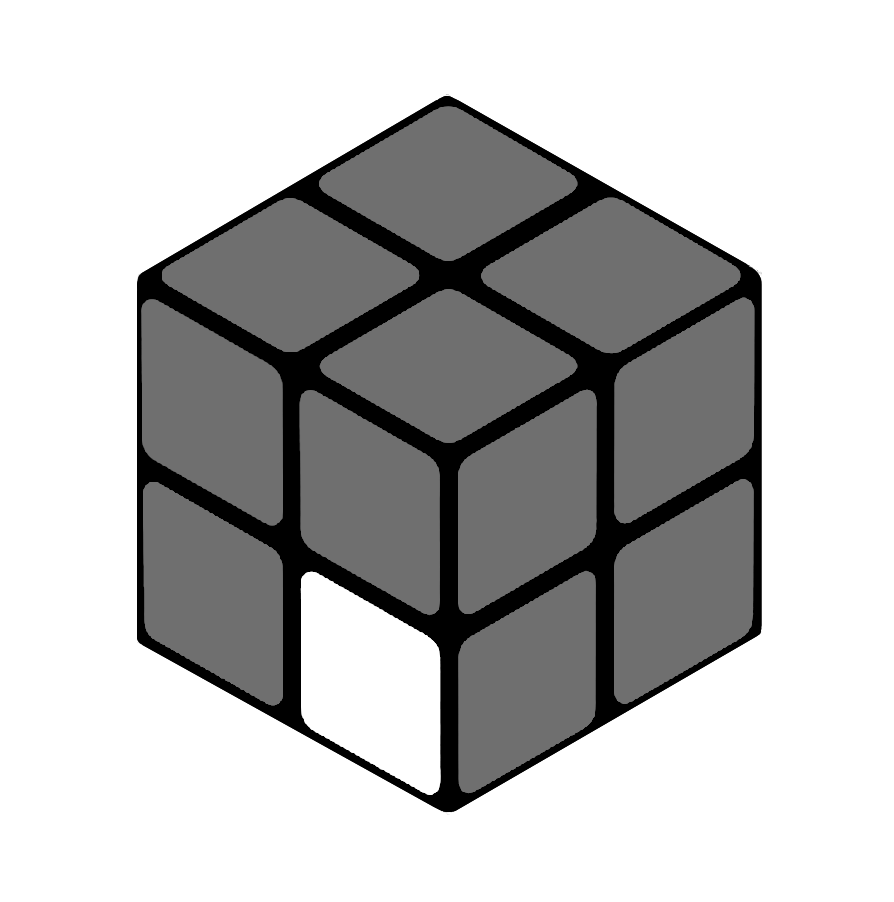
\includegraphics[scale=0.1]{e1_s1_s1.png}
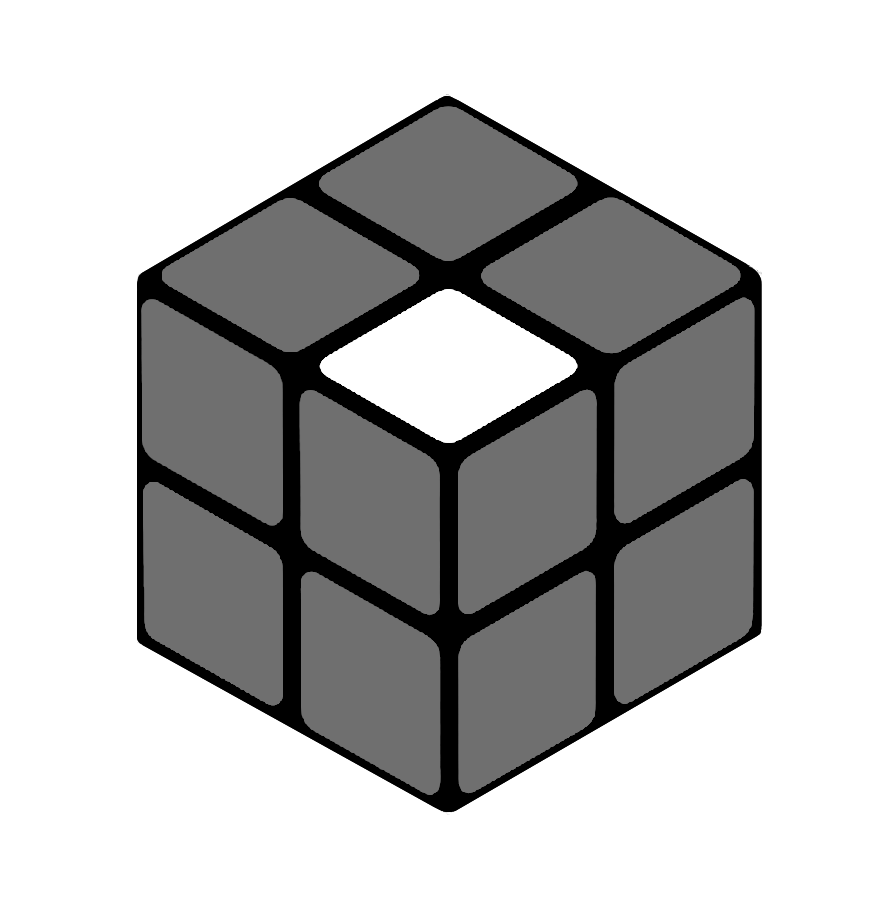
\includegraphics[scale=0.1]{e1_s1_s2.png}
\caption{ersten Eckstein positionieren}
\label{30}
\end{figure}

In Abbildung \ref{30} wird der erste Eckstein der oberen Ebene positioniert. Das kann dort entweder durch den Zug $R$ oder einer Rotation um die $y$-Achse passieren.

Der zweite Stein kann dann hinzugefügt werden. Es gibt für den \Ttwo Würfel Lösungsmethoden, bei denen man zuerst alle weißen Farbflächen ausrichten und dann die Steinposition anpasst.
Da hier aber Algorithmen des \Tthree Würfels übertragen werden, und man bei diesem die Steine der oberen Ebene üblicherweise direkt richtig ausrichtet und positioniert, wird hier auch so vorgegangen.
Die Farbfläche des zweiten Steins befindet sich für diesen Algorithmus seitlich an der unteren Ebene. (Optimalerweise befindet sich der Stein schon zufällig an der gewünschten, korrekten Position.)
Dann führt man $D$ aus, bis der Stein sich unter seiner Zielposition befindet und dreht ihn mit $L, R, F$ oder $R$ neben den bereits vorhandenen, ersten Eckstein. Das kann man auch in Abbildung \ref{31} sehen.

\begin{figure}[h]
\centering
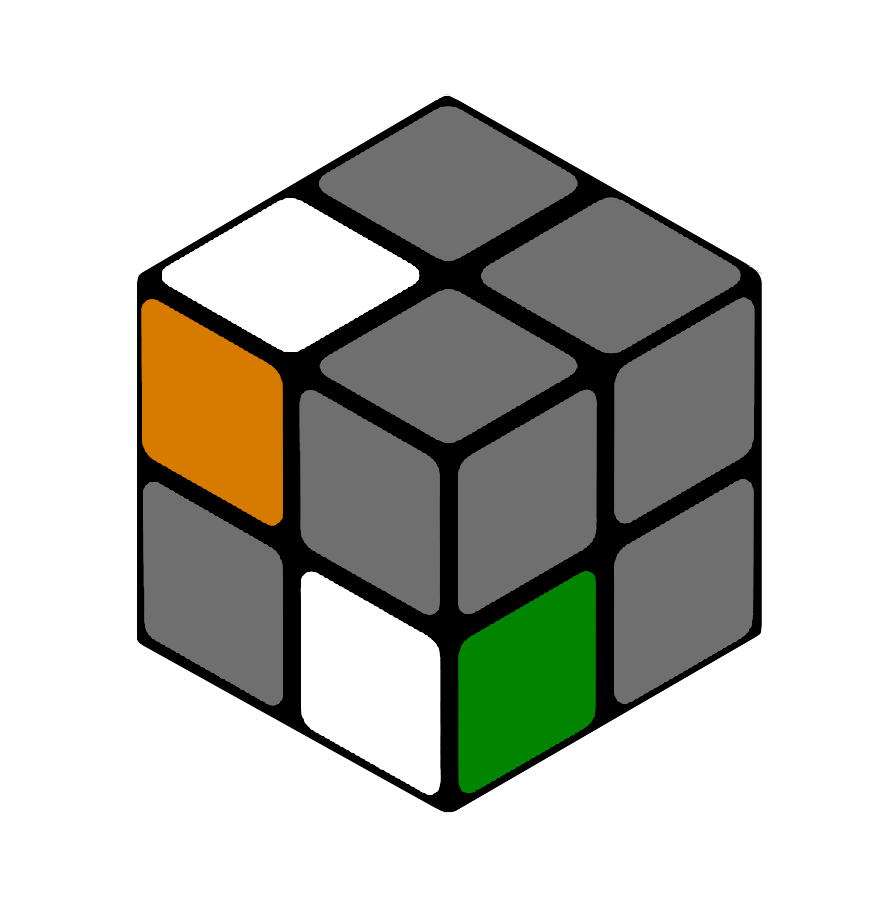
\includegraphics[scale=0.1]{e1_s2_s1.png}
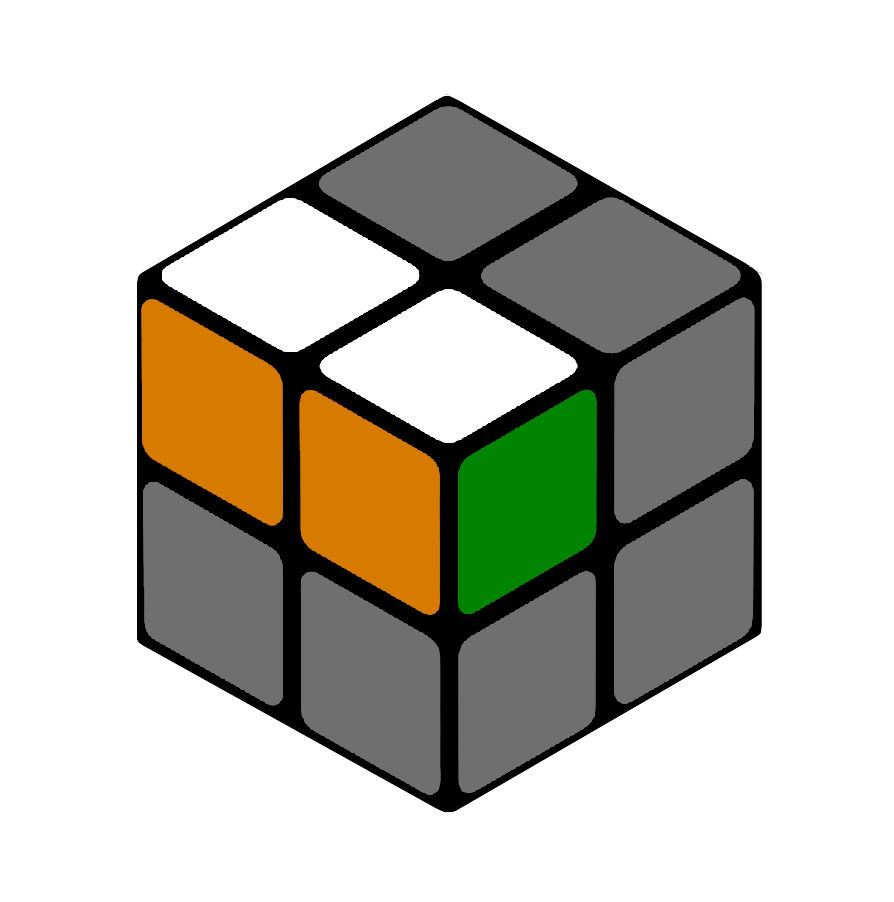
\includegraphics[scale=0.1]{e1_s2_s2.png}
\caption{zweiten Eckstein positionieren}
\label{31}
\end{figure}

Man sieht dort auch orange und grüne Farbflächen. Das gilt analog für die anderen benachbarten Farbflächen. Wichtig ist, dass die beiden Farbflächen einer Seite auch die gleiche Farbe haben.

Sollte die Farbfläche der Ecke unten am Würfel sein, so kann man sie falsch herum ausgerichtet mit der Technik aus Abbildung \ref{31} an die Position setzen. Dann befindet sich die weiße Farbfläche in der oberen Ebene, aber falsch herum ausgerichtet. Wenn das der Fall ist, kann man den Stein mit einem der Züge $L, R, F$ oder $B$ herausdrehen und mit $U$ in die untere Ebene schieben. Diesen Vorgang sieht man auch in Abbildung \ref{32}. Von dort kann man ihn mit der oben beschriebenen Technik richtig ausgerichtet und positioniert einfügen (s. Abbildung \ref{31}). 

\begin{figure}[h]
\centering
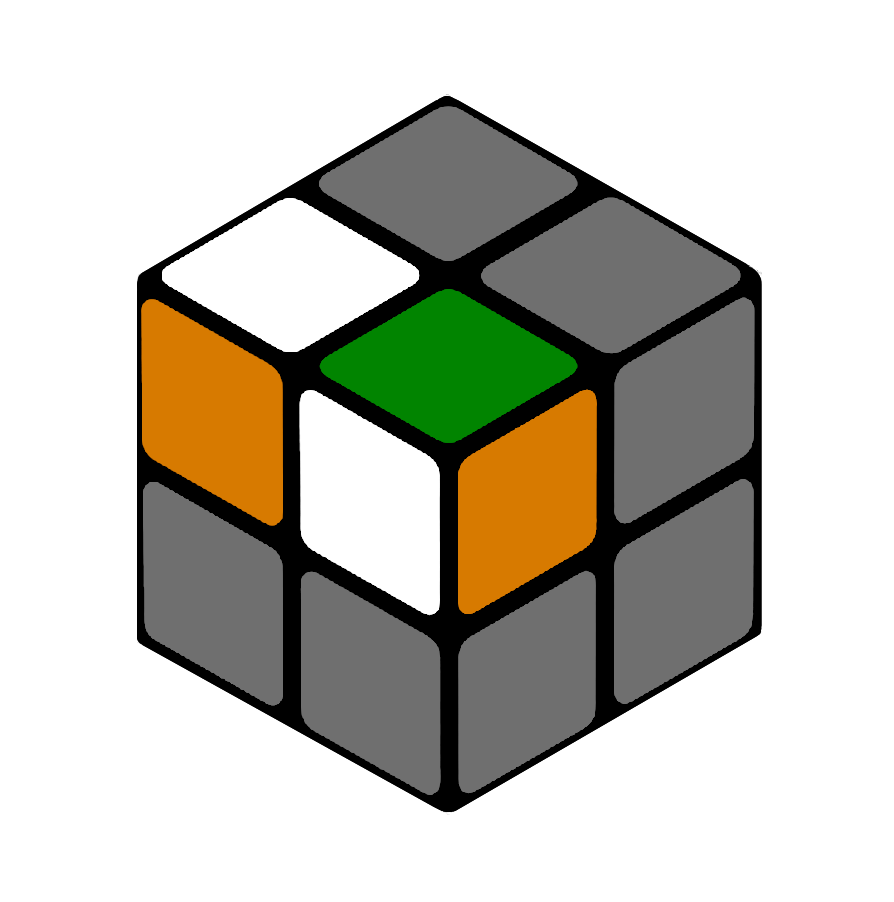
\includegraphics[scale=0.1]{e1_s2_s1_s.png}
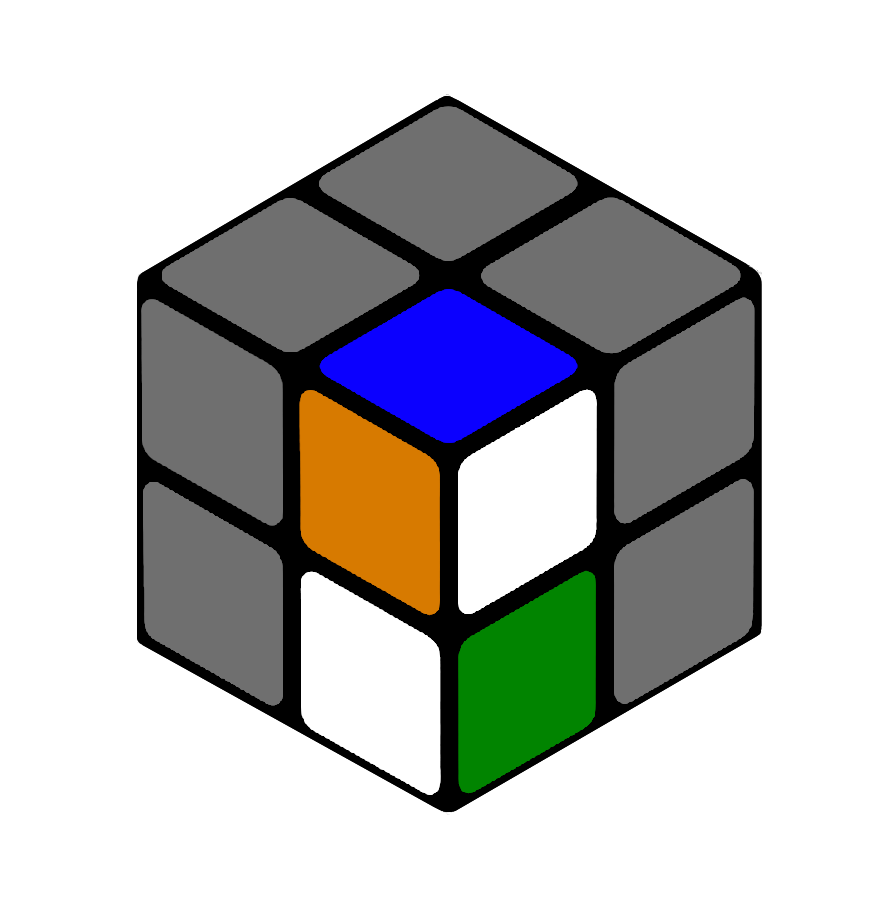
\includegraphics[scale=0.1]{e1_s2_s2_s.png}
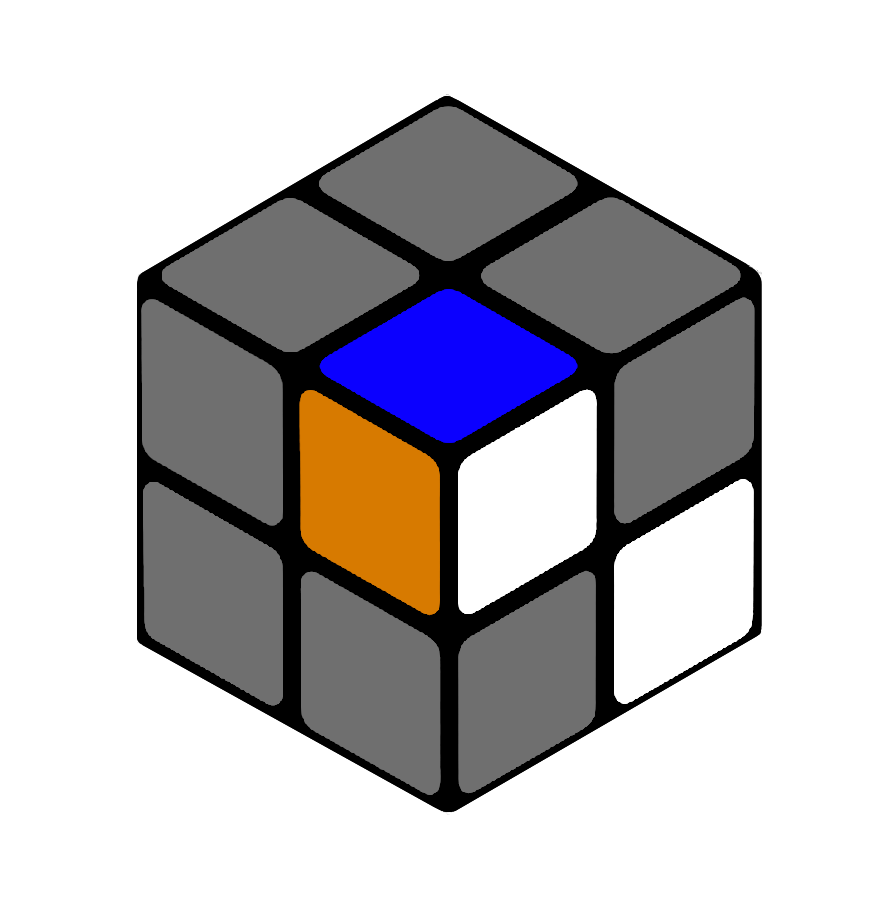
\includegraphics[scale=0.1]{e1_s2_s3_s.png}
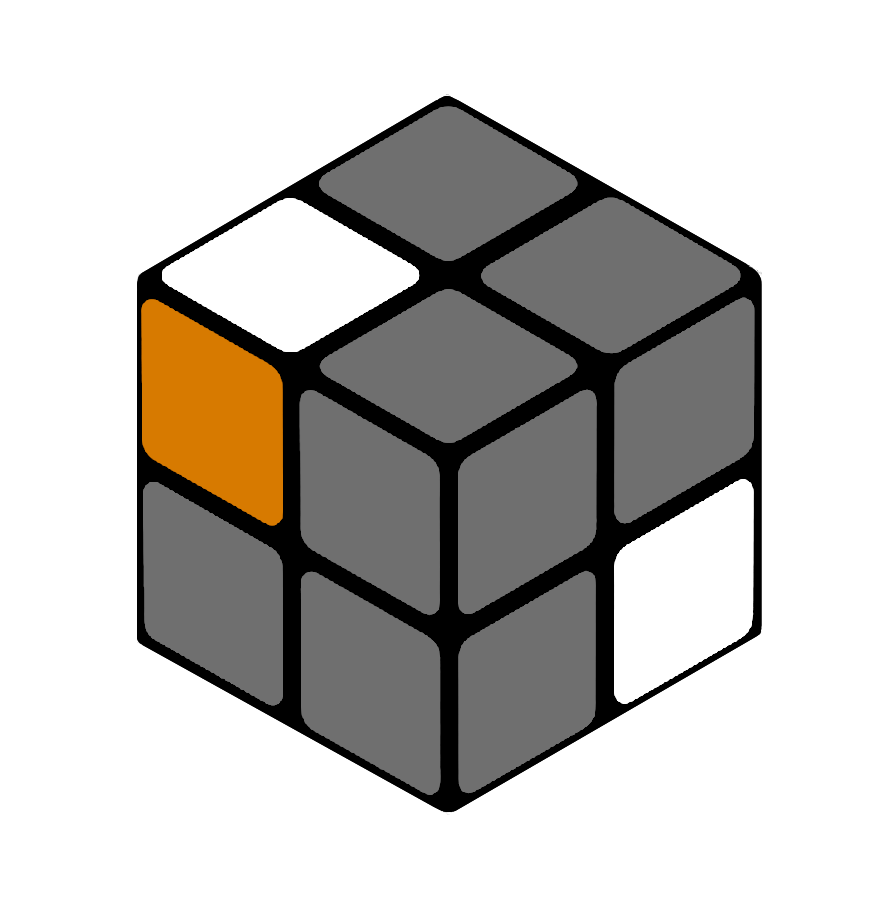
\includegraphics[scale=0.1]{e1_s2_s4_s.png}
\caption{zweiter Eckstein: Sonderfall}
\label{32}
\end{figure}

Die anderen zwei Steine der ersten Ebene lassen sich mit der oben genannten Technik ebenfalls positionieren. Die obere Ebene ist dann gelöst.
Bei dem \Ttwo Würfel entspricht das Lösen der oberen Ebene sogar schon der Hälfte des Würfels.



%
%
%
%
%
%
%
%
%
%=======================================================================================================
%
%
%
%
%
%
%
%
%
%
\subsection*{Algorithmen für die zweite Ebene}\addcontentsline{toc}{subsection}{\protect\numberline{}Algorithmen für die zweite Ebene}

\begin{figure}[h]
\centering
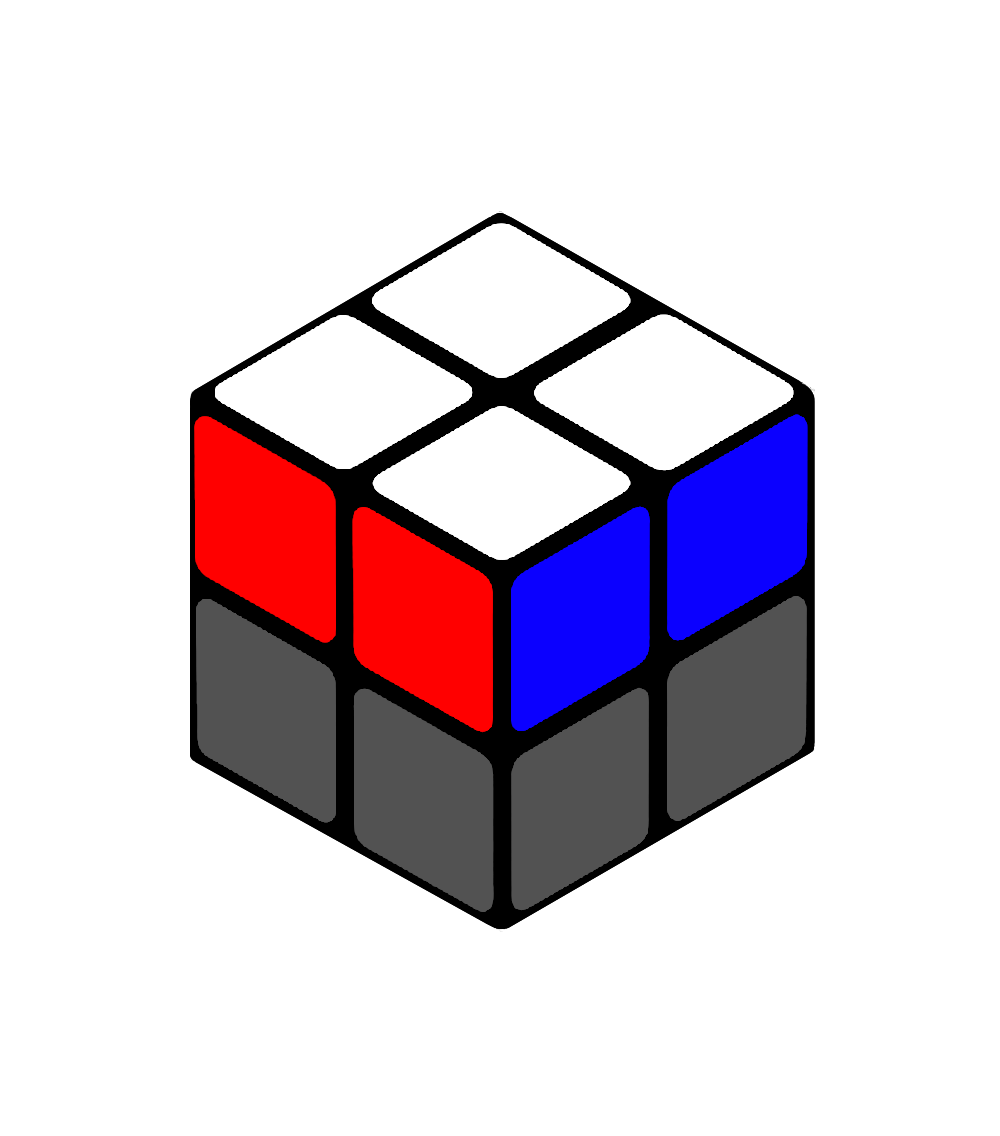
\includegraphics[scale=0.1]{ebene.png}
\caption{Würfel mit gelöster oberer Ebene}
\end{figure}

Beim Lösen der zweiten Ebene muss beachtet werden, die erste Ebene nicht wieder zu verdrehen. Deshalb sind die Algorithmen hier länger, um spezifische Steine zu bewegen.



%
%
%
%
%
%
%
%
%
%=======================================================================================================
%
%
%
%
%
%
%
%
%
%
\newpage


\begin{singlespacing}
\listoffigures
\end{singlespacing}



\newpage


\printbibliography









\end{document}














